% Options for packages loaded elsewhere
\PassOptionsToPackage{unicode}{hyperref}
\PassOptionsToPackage{hyphens}{url}
%
\documentclass[
]{article}
\usepackage{lmodern}
\usepackage{amssymb,amsmath}
\usepackage{ifxetex,ifluatex}
\ifnum 0\ifxetex 1\fi\ifluatex 1\fi=0 % if pdftex
  \usepackage[T1]{fontenc}
  \usepackage[utf8]{inputenc}
  \usepackage{textcomp} % provide euro and other symbols
\else % if luatex or xetex
  \usepackage{unicode-math}
  \defaultfontfeatures{Scale=MatchLowercase}
  \defaultfontfeatures[\rmfamily]{Ligatures=TeX,Scale=1}
\fi
% Use upquote if available, for straight quotes in verbatim environments
\IfFileExists{upquote.sty}{\usepackage{upquote}}{}
\IfFileExists{microtype.sty}{% use microtype if available
  \usepackage[]{microtype}
  \UseMicrotypeSet[protrusion]{basicmath} % disable protrusion for tt fonts
}{}
\makeatletter
\@ifundefined{KOMAClassName}{% if non-KOMA class
  \IfFileExists{parskip.sty}{%
    \usepackage{parskip}
  }{% else
    \setlength{\parindent}{0pt}
    \setlength{\parskip}{6pt plus 2pt minus 1pt}}
}{% if KOMA class
  \KOMAoptions{parskip=half}}
\makeatother
\usepackage{xcolor}
\IfFileExists{xurl.sty}{\usepackage{xurl}}{} % add URL line breaks if available
\IfFileExists{bookmark.sty}{\usepackage{bookmark}}{\usepackage{hyperref}}
\hypersetup{
  pdftitle={PRACTICA 2: LIMPIEZA Y VALIDACIÓN DE LOS DATOS},
  pdfauthor={Gines Molina e Iñigo Alvarez},
  hidelinks,
  pdfcreator={LaTeX via pandoc}}
\urlstyle{same} % disable monospaced font for URLs
\usepackage[margin=1in]{geometry}
\usepackage{color}
\usepackage{fancyvrb}
\newcommand{\VerbBar}{|}
\newcommand{\VERB}{\Verb[commandchars=\\\{\}]}
\DefineVerbatimEnvironment{Highlighting}{Verbatim}{commandchars=\\\{\}}
% Add ',fontsize=\small' for more characters per line
\usepackage{framed}
\definecolor{shadecolor}{RGB}{48,48,48}
\newenvironment{Shaded}{\begin{snugshade}}{\end{snugshade}}
\newcommand{\AlertTok}[1]{\textcolor[rgb]{1.00,0.81,0.69}{#1}}
\newcommand{\AnnotationTok}[1]{\textcolor[rgb]{0.50,0.62,0.50}{\textbf{#1}}}
\newcommand{\AttributeTok}[1]{\textcolor[rgb]{0.80,0.80,0.80}{#1}}
\newcommand{\BaseNTok}[1]{\textcolor[rgb]{0.86,0.64,0.64}{#1}}
\newcommand{\BuiltInTok}[1]{\textcolor[rgb]{0.80,0.80,0.80}{#1}}
\newcommand{\CharTok}[1]{\textcolor[rgb]{0.86,0.64,0.64}{#1}}
\newcommand{\CommentTok}[1]{\textcolor[rgb]{0.50,0.62,0.50}{#1}}
\newcommand{\CommentVarTok}[1]{\textcolor[rgb]{0.50,0.62,0.50}{\textbf{#1}}}
\newcommand{\ConstantTok}[1]{\textcolor[rgb]{0.86,0.64,0.64}{\textbf{#1}}}
\newcommand{\ControlFlowTok}[1]{\textcolor[rgb]{0.94,0.87,0.69}{#1}}
\newcommand{\DataTypeTok}[1]{\textcolor[rgb]{0.87,0.87,0.75}{#1}}
\newcommand{\DecValTok}[1]{\textcolor[rgb]{0.86,0.86,0.80}{#1}}
\newcommand{\DocumentationTok}[1]{\textcolor[rgb]{0.50,0.62,0.50}{#1}}
\newcommand{\ErrorTok}[1]{\textcolor[rgb]{0.76,0.75,0.62}{#1}}
\newcommand{\ExtensionTok}[1]{\textcolor[rgb]{0.80,0.80,0.80}{#1}}
\newcommand{\FloatTok}[1]{\textcolor[rgb]{0.75,0.75,0.82}{#1}}
\newcommand{\FunctionTok}[1]{\textcolor[rgb]{0.94,0.94,0.56}{#1}}
\newcommand{\ImportTok}[1]{\textcolor[rgb]{0.80,0.80,0.80}{#1}}
\newcommand{\InformationTok}[1]{\textcolor[rgb]{0.50,0.62,0.50}{\textbf{#1}}}
\newcommand{\KeywordTok}[1]{\textcolor[rgb]{0.94,0.87,0.69}{#1}}
\newcommand{\NormalTok}[1]{\textcolor[rgb]{0.80,0.80,0.80}{#1}}
\newcommand{\OperatorTok}[1]{\textcolor[rgb]{0.94,0.94,0.82}{#1}}
\newcommand{\OtherTok}[1]{\textcolor[rgb]{0.94,0.94,0.56}{#1}}
\newcommand{\PreprocessorTok}[1]{\textcolor[rgb]{1.00,0.81,0.69}{\textbf{#1}}}
\newcommand{\RegionMarkerTok}[1]{\textcolor[rgb]{0.80,0.80,0.80}{#1}}
\newcommand{\SpecialCharTok}[1]{\textcolor[rgb]{0.86,0.64,0.64}{#1}}
\newcommand{\SpecialStringTok}[1]{\textcolor[rgb]{0.80,0.58,0.58}{#1}}
\newcommand{\StringTok}[1]{\textcolor[rgb]{0.80,0.58,0.58}{#1}}
\newcommand{\VariableTok}[1]{\textcolor[rgb]{0.80,0.80,0.80}{#1}}
\newcommand{\VerbatimStringTok}[1]{\textcolor[rgb]{0.80,0.58,0.58}{#1}}
\newcommand{\WarningTok}[1]{\textcolor[rgb]{0.50,0.62,0.50}{\textbf{#1}}}
\usepackage{longtable,booktabs}
% Correct order of tables after \paragraph or \subparagraph
\usepackage{etoolbox}
\makeatletter
\patchcmd\longtable{\par}{\if@noskipsec\mbox{}\fi\par}{}{}
\makeatother
% Allow footnotes in longtable head/foot
\IfFileExists{footnotehyper.sty}{\usepackage{footnotehyper}}{\usepackage{footnote}}
\makesavenoteenv{longtable}
\usepackage{graphicx}
\makeatletter
\def\maxwidth{\ifdim\Gin@nat@width>\linewidth\linewidth\else\Gin@nat@width\fi}
\def\maxheight{\ifdim\Gin@nat@height>\textheight\textheight\else\Gin@nat@height\fi}
\makeatother
% Scale images if necessary, so that they will not overflow the page
% margins by default, and it is still possible to overwrite the defaults
% using explicit options in \includegraphics[width, height, ...]{}
\setkeys{Gin}{width=\maxwidth,height=\maxheight,keepaspectratio}
% Set default figure placement to htbp
\makeatletter
\def\fps@figure{htbp}
\makeatother
\setlength{\emergencystretch}{3em} % prevent overfull lines
\providecommand{\tightlist}{%
  \setlength{\itemsep}{0pt}\setlength{\parskip}{0pt}}
\setcounter{secnumdepth}{-\maxdimen} % remove section numbering
\ifluatex
  \usepackage{selnolig}  % disable illegal ligatures
\fi

\title{PRACTICA 2: LIMPIEZA Y VALIDACIÓN DE LOS DATOS}
\author{Gines Molina e Iñigo Alvarez}
\date{29/12/2020}

\begin{document}
\maketitle

{
\setcounter{tocdepth}{2}
\tableofcontents
}
\begin{Shaded}
\begin{Highlighting}[]
\CommentTok{\# Carga de librerías}
\KeywordTok{library}\NormalTok{(dplyr)}
\KeywordTok{library}\NormalTok{(VIM)}
\KeywordTok{library}\NormalTok{(gridExtra)}
\KeywordTok{library}\NormalTok{(ggplot2)}
\KeywordTok{library}\NormalTok{(stringi)}
\KeywordTok{library}\NormalTok{(stringr)}
\KeywordTok{library}\NormalTok{(tmaptools)}
\KeywordTok{library}\NormalTok{(polycor)}
\KeywordTok{library}\NormalTok{(reshape2)}
\KeywordTok{library}\NormalTok{(wordcloud)}
\KeywordTok{library}\NormalTok{(wordcloud2)}
\KeywordTok{library}\NormalTok{(viridis)}
\KeywordTok{library}\NormalTok{(scales)}
\KeywordTok{library}\NormalTok{(magrittr)}
\KeywordTok{library}\NormalTok{(forcats)}
\CommentTok{\# library(highcharter)}
\CommentTok{\# library(maps)}
\CommentTok{\# library(ggmap)}
\CommentTok{\# library(ggpubr)}
\CommentTok{\# library(tidyverse)}
\CommentTok{\# library(plotly)}
\end{Highlighting}
\end{Shaded}

\hypertarget{descripcion-del-dataset}{%
\section{1. Descripción del dataset}\label{descripcion-del-dataset}}

El dataset es un listado de ofertas de trabajo publicadas en Linkedin
para ciencia de datos (término ``Data Scientist'') que fue obtenido en
la primera parte de esta práctica.

Se ha decidido la utilización de este dataset ya que se trata de un
dataset propio que no ha sido ampliamente explotado a análisis y
queríamos tener una experiencia más cercana a lo que sería un proyecto
real. Se consiguen resultados y se llevan a cabo las técnicas que
queríamos aplicar para obtener las respuestas a nuestras preguntas sobre
el panorama de búsqueda de empleo.

Se pueden ver los datos y el código en el siguiente repositorio:
\url{https://github.com/InigoAB/DataCleaning}

Consta de 6 archivos CSV con las ofertas encontradas a nivel de Escocia,
Reino Unido, España, Mundo y remoto que unificaremos, limpiaremos y
daremos formato para posteriormente analizar y buscar información
relevante.

Trataremos de ir respondiendo a distintas preguntas que nos vayan
durgiendo como pueden ser las siguientes: - ¿Qué variables son
relevantes? - ¿Que diferencias hay segun la localizacion o paises? - ¿Es
una opción los puestos en Remoto? - ¿Hay diferencias entre latitudes
positivas y negativas? - ¿Existe correlación entre si hay quick
application y si se trata de una empresa grande o no? - ¿Existe
correlacion entre el tipo de puesto y el numero de solicitudes? - ¿Qué
tipo de puestos de trabajo prioriza LinkedIn en sus resultados? - ¿Qué
palabras son las más utilizadas en las descripciones de las ofertas de
trabajo?

\hypertarget{integracion-y-seleccion-de-los-datos-de-interes-a-analizar}{%
\section{2. Integración y selección de los datos de interés a
analizar}\label{integracion-y-seleccion-de-los-datos-de-interes-a-analizar}}

El primer paso es integrar los archivos de las distintas ubicaciones en
un mismo dataframe con el que podamos trabajar.

\begin{Shaded}
\begin{Highlighting}[]
\NormalTok{Scotland \textless{}{-}}\StringTok{ }\KeywordTok{read.csv}\NormalTok{(}\StringTok{"data/Scotland.csv"}\NormalTok{, }\DataTypeTok{header=}\OtherTok{TRUE}\NormalTok{, }\DataTypeTok{sep=}\StringTok{","}\NormalTok{, }\DataTypeTok{stringsAsFactors=}\OtherTok{FALSE}\NormalTok{)}
\NormalTok{Spain \textless{}{-}}\StringTok{ }\KeywordTok{read.csv}\NormalTok{(}\StringTok{"data/Spain.csv"}\NormalTok{, }\DataTypeTok{header=}\OtherTok{TRUE}\NormalTok{, }\DataTypeTok{sep=}\StringTok{","}\NormalTok{, }\DataTypeTok{stringsAsFactors=}\OtherTok{FALSE}\NormalTok{)}
\NormalTok{UK \textless{}{-}}\StringTok{ }\KeywordTok{read.csv}\NormalTok{(}\StringTok{"data/UK.csv"}\NormalTok{, }\DataTypeTok{header=}\OtherTok{TRUE}\NormalTok{, }\DataTypeTok{sep=}\StringTok{","}\NormalTok{, }\DataTypeTok{stringsAsFactors=}\OtherTok{FALSE}\NormalTok{)}
\NormalTok{WorldWide \textless{}{-}}\StringTok{ }\KeywordTok{read.csv}\NormalTok{(}\StringTok{"data/WorldWide.csv"}\NormalTok{, }\DataTypeTok{header=}\OtherTok{TRUE}\NormalTok{, }\DataTypeTok{sep=}\StringTok{","}\NormalTok{, }\DataTypeTok{stringsAsFactors=}\OtherTok{FALSE}\NormalTok{)}
\NormalTok{Remote \textless{}{-}}\StringTok{ }\KeywordTok{read.csv}\NormalTok{(}\StringTok{"data/Remote.csv"}\NormalTok{, }\DataTypeTok{header=}\OtherTok{TRUE}\NormalTok{, }\DataTypeTok{sep=}\StringTok{","}\NormalTok{, }\DataTypeTok{stringsAsFactors=}\OtherTok{FALSE}\NormalTok{)}
\NormalTok{Scotland}\OperatorTok{$}\NormalTok{dataset \textless{}{-}}\StringTok{ "Scotland"}
\NormalTok{Spain}\OperatorTok{$}\NormalTok{dataset \textless{}{-}}\StringTok{ "Spain"}
\NormalTok{UK}\OperatorTok{$}\NormalTok{dataset \textless{}{-}}\StringTok{ "UK"}
\NormalTok{WorldWide}\OperatorTok{$}\NormalTok{dataset \textless{}{-}}\StringTok{ "WorldWide"}
\NormalTok{Remote}\OperatorTok{$}\NormalTok{dataset \textless{}{-}}\StringTok{ "Remote"}
\NormalTok{jobs \textless{}{-}}\StringTok{ }\KeywordTok{rbind}\NormalTok{(Scotland, Spain, UK, WorldWide, Remote)}
\KeywordTok{dim}\NormalTok{(jobs)}
\end{Highlighting}
\end{Shaded}

\begin{verbatim}
## [1] 3456   18
\end{verbatim}

Obtenemos un dataframe de 3456 observaciones y 18 variables.

Vemos las primeras observaciones del mismo.

\begin{Shaded}
\begin{Highlighting}[]
\KeywordTok{head}\NormalTok{(jobs)}
\end{Highlighting}
\end{Shaded}

\begin{verbatim}
##   X     Job.ID       Date Company.Name                    Title
## 1 0 2011662890 2020-10-15      Dufrain            Data Engineer
## 2 1 2227320776 2020-10-30 Sopra Steria          User Researcher
## 3 2 2201826818 2020-10-22    Sword ITS            Data Engineer
## 4 3 2284269209 2020-11-05         None Data Scientist - Glasgow
## 5 4 2264114504 2020-10-16     Experian           Data Scientist
## 6 5 2249308521 2020-10-11      Harnham           Data Scientist
##                              Location
## 1 Edinburgh, Scotland, United Kingdom
## 2 Edinburgh, Scotland, United Kingdom
## 3  Aberdeen, Scotland, United Kingdom
## 4                         Glasgow, GB
## 5                         Glasgow, GB
## 6                         Glasgow, GB
##                                                                                                                                                                                                                                                                                                                                                                                                                                                                                                                                                                                                                                                                                                                                                                                                                                                                                                                                                                                                                                                                                                                                                                                                                                                                                                                                                                                                                                                                                                                                                                                                                                                                                                                                                                                                                                                                                                                                                                                                                                                                                                                                                                                                                                                                                                                                                                                                                                                                                                                                                                                                                                                                                                                                                                                                                                                                                                                                                                                                                                                                                                                                                                                                                                                                                                                                                                                                                                                                                                                                                                                                                                                                                                                                                                                                                                                                                                                                                                                                                                                                                                                                                                                                                                                                                                                                                                                                                                                                                                                                                                                                                                                                                                                                                                                                                                                                                                                                                                                                                                                                                                                                                                                                                                             Description
## 1                                                                                                                                                                                                                                                                                                                                                                                                                                                                                                                                                                                                                                                                                                                                                                                                                                                                                                                                                                                                                                                                                                                                                                                                                                                                                                                                                                                                                                                                                                                                                                                                                                                                                                                                                                                                                                                                                                                             Data Engineer London, Edinburgh OR Manchester   We are Dufrain. We’re a market-leading Data Management, Analytics and BI consultancy with offices across the UK, working with some of the biggest names in the Financial Services industry. We are proud to be an agile, client focused consultancy where we all share a common goal.  As we continue to build and strengthen our capability, a number of exciting opportunities have arisen to join our market-leading Data Management and Analytics Consultancy. We are looking for dynamic individuals, with proven experience and strong technical skills to join our teams in our Edinburgh, London and Manchester offices.  What we offer you: Working as a Data Engineer at Dufrain you’ll have the opportunity to work with a creative and highly skilled team of consultants who have expertise in technical delivery, technologies and concepts in areas such as Data Storage, Data Ingestion, Data Integration, Data Warehousing, Data Preparation and Cloud Infrastructure. You will also have your own ‘people coach’ to guide and support you with your career journey with us. Dufrain offers an autonomous environment where you have opportunities to have access to training tools & technical community groups and provides multi sector and international client exposure.    Who we’re looking for: we are looking for Data Engineers who have a genuine interest of rich data and have experience on delivery that contributes to wider business outcomes and be able to concisely articulate to stakeholders and interested parties their role and solutions in a way that can be easily understood.   Essential Requirements: Strong cloud engineering experience  Skilled in multiple languages such as SQL, Python, Java, Scala, Julia Hands on experience of cloud platforms such as Azure, AWS & GCP - (Certified to practitioner level in at least one provider) Experience working with one or more of the tools - Spark, Kafka, Snowflake, Hadoop Experience working with both SQL and NoSQL foundational tools and databases such as Cassandra, MongoDB  Experience delivering multiple solutions using key techniques such as Data Modelling, DWH, Lakes, ETL, ELT, Virtualisation & Streaming Solid knowledge of development principles such as ETL, DWH & Streaming  Minimum 2 years’ experience as Data Engineer with previous experience in industry or as SQL developer Flexibility to travel to and work on client sites within the UK and occasionally Europe Excellent track record in executive stakeholder management and maintaining valuable relationships. Takes ownership and accountability for critical initiatives and deliverables both internally and for clients Awareness of current market trends in data having the ability to influence opinion and decisioning across the Data Management spectrum A passionate desire and attitude to learn new tools  What to do next: Please apply via the application link below. Once your application has been received a representative from the Dufrain Recruitment team will review your profile and inform you of the next steps.   Please note: The recruitment process will require any candidates that are shortlisted to complete an online technical assessment.
## 2 Bring your User Research expertise to us and in return we’ll give you an amazing career with growth and learning opportunities. Come and work for one of the best kept secrets in I.T.  The companySopra Steria, European leader in digital transformation, provides one of the most comprehensive portfolios of end-to-end service offerings in the market: Consulting, Systems Integration, Software Development and Business Process Services. Sopra Steria is a trusted by leading private and public organisations to deliver successful transformation programmes that address their most complex and critical business challenges. The day jobCurrently looking for a User Researcher for a unique opportunity to work within an established project team. The successful candidate will be confident in applying team research methods in support of user research initiatives as well as identifying opportunities for methods improvement and development.   Responsibilities will include:Data analysis – Collects and analyses data related to people’s behaviours, needs, and opinionsGenerates insights – Supports synthesis of findings and the creation of insights, reports and presentations to inform decision making and drive actions at a project levelPrioritise requirements – Provides constructive challenge and enables effective prioritisation of requirements from user needs based on evidence from researchTools – Contributes to selection of the user research approaches for projects and initiatives and can plan and execute own user research activities as requiredCommunicate findings – Can synthesise and articulate research findings clearly and effectively. Identifies appropriate opportunities for publication and dissemination of research findings. Develops and shares practical demonstrations of research findings. Presents papers at conferences, contribute material of publication quality, and presents reports to clientsUsability tests – Can design and deliver usability testsResearch Ethics – Is able to follow a research ethics plan, and generate appropriate ethics documentation for a range of projects, understands the application of GDPR to the storage and use of participant information, and data privacyUser recruitment – Can recruit participants for project, taking into account diversity, appropriate samples and how best to address project team prioritiesUser Data Security – Stores participant information securely, using an established systemBuild empathy – Helps client and colleagues empathise with the user, through tools such as mental models/ empathy maps/ personas or user case studiesResearch Practice – Is confident working with a range of users, in different contexts, e.g. one-to-one interviews, workshops, focus groups, ethnographic research   Essential Skills: (Design and Technical Skills)Design for user needs – Is able to identify, describe and design for user needs, including a comprehensive awareness of accessibility needs and ensuring that user stories are well defined Prototype analysis – Is confident evaluating prototypes or designs of systems, products or services against the agreed usability and accessibility specifications. Can interpret and present results of evaluations and prioritises issues UX support – Has a solid understanding of core UX tools and techniques Design systems – Is able to interpret and understand design systems Design user experience – Understands and applies UX design learning Impact analysis – Plan and undertake analysis to help design decisions and understand their trade-offs Design Standards – Is confident working within pre-defined standards (e.g. legal, regulatory or design system criteria). Can contribute to the development of policies and standards related to design decisions and technology choicesAccessibility – Confident in applying accessibility criteria into designs and providing rationale and advice and guidance onto project and programmesInnovation – Is able to identify, capture and communicate innovation opportunities within individual and across different projects Desirable Skills:Team support – Providing peer review support for UX team. Team Assets – Ensures capture of relevant tools, techniques and templates into asset library. Supports with authoring of new materialEvents – Books and organises learning events for team and/or organisation. Individual expertise – Develop an area of personal expertise Reasons why you should apply to usWe’re big – really big. With that comes career growth opportunities - we offer excellent training, you’ll join a company where development and progression is actively encouraged and not just something we talk aboutWe have an enviable client list – we work with some of the biggest names out thereWe ensure our working environment is supportive and collaborative, everyone has a voice and all opinions count Our goal is to disrupt the market, not just follow the status quoSustainability is really important to us, in fact we are within the top 1% of companies worldwide tackling climate change and managing our emissions
## 3                                                                                                                                                                                                                                                                                                                                                                                                                                                                                                                                                                                                                                                                                                                                                                                                                                                                                                                                                                                                                                                                                                                                                                                                                                                                                                                                                                                                                                                                                                                                                                                                                                                                                                                                                                                                                                                                                                                                                                                                                                                                                                                                                                                                                                                                                                                                    Sword are a trusted partner to a significant number of Oil & Gas sector clients in the UK. Our Aberdeen based Energy Services team employs talented individuals who deliver Information Technology and Data Management solutions, leveraging the latest developments in systems and technology, whilst delivering a consistently first-class service to our customers. As the pre-eminent provider of Information Technology services to the Energy Sector in Aberdeen, we have an excellent opportunity for junior level Data Engineer to join our busy team on a permanent staff basis. Job Purpose Successful delivery of Power BI, especially in support of Citizen Developers, requires addressing frequent requests for new or additional data to be added to the Data Warehouse.  This role will help ensure the successful delivery of digital projects to the business by working closely with our customer's business including business analysts, the data architect and system owners to identify and prepare source data for use in the data warehouse. You will be required to: Understand, extract and transform data from a variety of source systems and load it into the enterprise data warehouse.Work as part of a technical team for digital analytic data delivery.Understand and participate in business and functional requirements to ensure data can deliver business value.Collaborate with fellow developers and business representatives to solve problems.Follow design and coding guidelines and offer suggestions for improvement.Review extract code and assist fellow team members in delivery.Document data extraction process. Education Graduate or equivalent in IT or science discipline preferred but not essential.Ideally you should have some oil and gas industry experience in an IT environment. Technical Skills Strong SQL knowledge and source data analysis skills and data modelling skills.Able to communicate with technical and the non-technical people.Hands-on experience in full ETL lifecycle:Source data analysis.Data development process.Data integration design.Dimensional data modelling.Demonstrable experience in extracting data from source systems and populating a data warehouse is essential.Experience in SQL Server 2016 TSQL, Analysis Services (preferably tabular to multidimensional).Experience with data visualisation tools, (Power BI) an advantage.Experience using TimeXtender Discovery Hub an advantage.Azure data lake, data factory and other applications on the Azure data platform an advantage.Big Data experience an advantage. Interpersonal Skills Confident, enthusiastic and strong communication capabilityTakes responsibility and delivers.A self-starter able to work alone and as part of a small team.  For a confidential discussion regards this opportunity please apply on-line in the first instance.
## 4                                                                                                                                                                                                                                                                                                                                                                                                                                                                                                                                                                                                                                                                                                                                                                                                                                                                                                                                                                                                                                                                                                                                                                                                                                                                                                                                                                                                                                                                                                                                                                                                                                                                                                                                                                                                                                                                                                                                                                                                                                                                                                                                                                                                                    Data Scientist – Glasgow  This advanced Software House are looking to recruit a Data Scientist who will be developing Microsoft Azure-hosted machine learning (SaaS) algorithms, the main aim of the role for the Data Scientist will be applying data mining techniques, carrying out statistical analysis and building high quality machine learning prediction systems integrated with their product. While a theoretical/academic knowledge of machine learning is important, our ideal candidate is someone who can translate this into real world solutions that deliver quantified business benefit. Core responsibilities for this Data Scientist role: Collaborate with the Product Owner, development team and other key stakeholders to define the roadmap, understand the role that machine learning / analytics has in achieving this roadmap and size the work appropriately.Work as an integral member of a Scrum team to deliver iterative functionality and enhanced data analytics.Take additional external data sources into their solution and extend the machine learning algorithms to improve our prediction models:Feeds of data from IoT devices / Azure IoT Hub and 3rd party cloud services.Data Mining.Data Analytics.Evaluation, selection and training of Machine Learning models within Azure.Development, Configuration and Deployment of Machine Learning models to Azure (as containers).Processing, cleansing, and verifying the integrity of data used for analysis.Doing ad-hoc analysis and presenting results in a clear manner to help inform product direction. Core skills & experienceExcellent understanding of machine learning techniques and algorithms.Proven ability to evaluate multiple machine learning algorithms against varying data sets and determine which algorithms will yield the best results.Knowledge of Azure Machine Learning SaaS-based services, including model selection, training, configuration and deployment.Experience displaying and analysing data using PowerBI.Experience with common data science toolkitsProficiency in using SQL for querying data.Good applied statistics skills, such as distributions, statistical testing, regression, etc. The role will appeal to an individual capable of working in a fast paced environment, the Data Scientist will have the initiative to approach challenges with enthusiasm and the ability to react to changes whilst maintaining a clear focus on the company objectives. Exceptional time management, communication and problems solving skills are a must. Keywords: Data Scientist, Azure, SaaS, Machine learning, algorithms, Data Analytics, Data Mining, Data analysis, SQL, PowerBI, Glasgow, Renfrewshire, Paisley, Scotland, Port Of Glasgow, Clydebank, Azure Send your CV to Bethany now – (url removed) or call (phone number removed)Please follow us on twitter @erinassociates for similar roles Erin Associates Ltd is acting as an Employment Agency in relation to this vacancy
## 5                                                                                                                                                                                                                                                                                                                                                                                                                                                                                                                                                                                                                                                                                                                                                                                                                                                                                                                                                                                                                                                                                                                                                                                                                                                                                                                                                                                                                                                                                                                                               Data Scientist  Castlight - Experian Digital   Location: Glasgow, Flexible  In Castlight - Experian Digital, we create powerful tools that allow our clients to gain insights into their customers and markets enabling safer and lower risk decisioning. We enable tooling around affordability and safe lending which ultimately helps end users. This section of the business is growing and we are in the unique position to collaborate directly with large clients in banking who are eager to consume our services, as well as combine Open Banking and other data with advanced class-leading data science products and classic bureau data.  Responsibilities  Develop and maintain data processes and models to support Castlight data products, e.g. CastScore, Income Insights and CaaS Create, review and maintain datasets for use in Castlight data products, e.g. manually classify CaaS training set data Continually learn and develop the knowledge and skills to process, manipulate and analyse data used in Castlight data products Work with data science colleagues to peer review and constructively challenge work done in the team Collaborate with subject matter experts outside the team to improve the customer experience and outcomes Work with clients to gather data requirements, execute proof of concept activities, and provide expertise to support the usage of Castlight data products Put Castlight’s vision of a safer financial world at the heart of every decision, consistent with Castlight’s People, Technology and Vision values   What Makes This Role Special  Affordability is a key topic in this challenging environment and as a provider of data services primarily around banking, affordability, and finance to other businesses we’re positioned to leverage Experian’s strong partnership with banks to make a genuine difference to real people in the country, and eventually internationally. Experian Digital regards Data Science as strategically important and is in a position of strong growth, and as such a positions in this team can achieve a high profile for performing individuals.  Could this role be for you?   Skills And Experience  Python for machine learning and data manipulation (sklearn, pandas, numpy, scipy, flask)  Docker/Kubernetes SQL for data access and retrieval Excel for data analysis Github for version control/collaboration Presentation and report writing  Why choose us?  Our colleagues’ health and wellbeing is a top priority for us, that’s why our reward, benefits and wellbeing programmes are designed so you can come to work feeling your very best self. Our benefits focus on health, money and lifestyle so you can tailor your benefits to your own personal needs. Whether it’s your physical and mental wellness, getting to work or planning for the future, we have a range of flexible options to have you covered!  Who are Experian?  We unlock the power of data to create opportunities for consumers, businesses and society. At life’s big moments – from buying a home or car, to sending a child to university, to growing a business exponentially by connecting it with new customers – we empower consumers and our clients to manage their data with confidence so they can maximize every opportunity.  For more than 125 years, we’ve helped consumers and clients prosper, and economies and communities flourish – and we’re not done.  Our 17,200 people in 44 countries believe the possibilities for you, and our world, are growing. We’re investing in new technologies, talented people and innovation so we can help create a better tomorrow.
## 6                                                                                                                                                                                                                                                                                                                                                                                                                                                                                                                                                                                                                                                                                                                                                                                                                                                                                                                                                                                                                                                                                                                                                                                                                                                                                                                                                                                                                                                                                                                                                                                                                                                                                                                                                                                                                                                                                                                                                                                                                                                                                                                                                                                                                                                                                                                                                                                                                                                                                                                                                                                                                                                                                                                                                                                                                                                                                                                                                                                                                                                                                                                                                                                                                                                                                                                                                                                                                                                                                                                                                                                                                                                                                         DATA SCIENTIST   £60000 + BENEFITS  GLASGOW  PYTHON, SCALA, SPARK   A new and exciting role has come available to work with a global market leader within the financial sector. As a data scientist you will help develop, tune and test data pipelines for various profiles. You will have the opportunity to use market-leading technology, using python, scala and spark.  The Company  As a data scientist you will sit within the financial crime analytics and data science team of one of the largest financial companies in the U.K. They are a dedicated and hardworking team that believe in service, and excellence.  THE ROLE   You will be working simultaneously with the financial crime and technology teams to assist with the execution of Quantexa capabilities as well as assisting with the development, tuning, and testing of data pipelines. You will develop, configure, and redesign these data pipelines using Scala and Spark. In addition, you will work closely with stakeholders across financial intelligence and global investigators.  Your Skills And Experience  The successful candidate will have the following skills and experience: Experience building analytic pipelinesExperience working with python and pysparkExtensive hands on programming experience of Scala and Spark  The Benefits  The successful Data Scientist will receive, depending on experience, a salary of up to £60,000  How To Apply  Please register your interest by sending your CV to Georgina Garraway via the Apply link on this page.
##             Level             Type
## 1      Intermedio Jornada completa
## 2      Intermedio Jornada completa
## 3 Sin experiencia Jornada completa
## 4 Sin experiencia Jornada completa
## 5 Sin experiencia Jornada completa
## 6 Sin experiencia Jornada completa
##                                             Functions
## 1            Tecnología de la información, Ingeniería
## 2                        Tecnología de la información
## 3 Tecnología de la información, Análisis, Consultoría
## 4            Ingeniería, Tecnología de la información
## 5            Ingeniería, Tecnología de la información
## 6            Ingeniería, Tecnología de la información
##                                                                               Industries
## 1              Servicios y tecnologías de la información, Banca, Servicio de información
## 2                                              Servicios y tecnologías de la información
## 3 Servicio de información, Servicios y tecnologías de la información, Petróleo y energía
## 4  Servicios y tecnologías de la información, Software, Dotación y selección de personal
## 5             Servicios y tecnologías de la información, Software, Servicios financieros
## 6                                Marketing y publicidad, Software, Servicios financieros
##   Solicitudes     Empleados Quick.Application Emails Visualizaciones
## 1          54        51-200             False                    679
## 2          30 Más de 10.001             False                    169
## 3          71        51-200              True                    325
## 4        None          None             False                      5
## 5          10 Más de 10.001             False                     98
## 6        None        51-200             False                      4
##        Recommended.Flavor  dataset
## 1 ACTIVELY_HIRING_COMPANY Scotland
## 2 ACTIVELY_HIRING_COMPANY Scotland
## 3 ACTIVELY_HIRING_COMPANY Scotland
## 4                    None Scotland
## 5         COMPANY_RECRUIT Scotland
## 6 ACTIVELY_HIRING_COMPANY Scotland
\end{verbatim}

Vamos a inspeccionar las variables.

\begin{Shaded}
\begin{Highlighting}[]
\KeywordTok{str}\NormalTok{(jobs)}
\end{Highlighting}
\end{Shaded}

\begin{verbatim}
## 'data.frame':    3456 obs. of  18 variables:
##  $ X                 : int  0 1 2 3 4 5 6 7 8 9 ...
##  $ Job.ID            : chr  "2011662890" "2227320776" "2201826818" "2284269209" ...
##  $ Date              : chr  "2020-10-15" "2020-10-30" "2020-10-22" "2020-11-05" ...
##  $ Company.Name      : chr  "Dufrain" "Sopra Steria" "Sword ITS" "None" ...
##  $ Title             : chr  "Data Engineer" "User Researcher" "Data Engineer" "Data Scientist - Glasgow" ...
##  $ Location          : chr  "Edinburgh, Scotland, United Kingdom" "Edinburgh, Scotland, United Kingdom" "Aberdeen, Scotland, United Kingdom" "Glasgow, GB" ...
##  $ Description       : chr  "Data Engineer London, Edinburgh OR Manchester   We are Dufrain. We’re a market-leading Data Management, Analyti"| __truncated__ "Bring your User Research expertise to us and in return we’ll give you an amazing career with growth and learnin"| __truncated__ "Sword are a trusted partner to a significant number of Oil & Gas sector clients in the UK. Our Aberdeen based E"| __truncated__ "Data Scientist – Glasgow  This advanced Software House are looking to recruit a Data Scientist who will be deve"| __truncated__ ...
##  $ Level             : chr  "Intermedio" "Intermedio" "Sin experiencia" "Sin experiencia" ...
##  $ Type              : chr  "Jornada completa" "Jornada completa" "Jornada completa" "Jornada completa" ...
##  $ Functions         : chr  "Tecnología de la información, Ingeniería" "Tecnología de la información" "Tecnología de la información, Análisis, Consultoría" "Ingeniería, Tecnología de la información" ...
##  $ Industries        : chr  "Servicios y tecnologías de la información, Banca, Servicio de información" "Servicios y tecnologías de la información" "Servicio de información, Servicios y tecnologías de la información, Petróleo y energía" "Servicios y tecnologías de la información, Software, Dotación y selección de personal" ...
##  $ Solicitudes       : chr  "54" "30" "71" "None" ...
##  $ Empleados         : chr  "51-200" "Más de 10.001" "51-200" "None" ...
##  $ Quick.Application : chr  "False" "False" "True" "False" ...
##  $ Emails            : chr  "" "" "" "" ...
##  $ Visualizaciones   : chr  "679" "169" "325" "5" ...
##  $ Recommended.Flavor: chr  "ACTIVELY_HIRING_COMPANY" "ACTIVELY_HIRING_COMPANY" "ACTIVELY_HIRING_COMPANY" "None" ...
##  $ dataset           : chr  "Scotland" "Scotland" "Scotland" "Scotland" ...
\end{verbatim}

Quitamos la primera columna ya que no es más que un índice que no aporta
ninguna información.

\begin{Shaded}
\begin{Highlighting}[]
\NormalTok{jobs}\OperatorTok{$}\NormalTok{X \textless{}{-}}\StringTok{ }\OtherTok{NULL}
\end{Highlighting}
\end{Shaded}

Todas las demás variables han quedado como de tipo carácter así que en
el siguiente apartado haremos las transformaciones necesarias, de
momento las explicamos.

\hypertarget{explicaciuxf3n-de-las-variables}{%
\subsection{Explicación de las
variables}\label{explicaciuxf3n-de-las-variables}}

Nos quedamos con las siguientes columnas - Job\_ID: identificador de la
oferta de empleo - Date: fecha de publicación - Company\_Name: nombre de
la empresa - Role: título o puesto de la oferta - Location: ubicación
del puesto - Description: descripción del puesto (del que se puede
extraer más información) - Level: nivel de experiencia requerida para el
puesto - Type: tipo de contrato (jornada completa o parcial) -
Functions: funciones del puesto de la oferta - Industries: sectores que
involucra - Solicitudes: número de solicitudes enviadas a la oferta -
Empleados: intervalo/número de empleados de la empresa - Quick
Application (True/False): método de solicitud rápida por LinkedIn
Emails: e-mails de contacto - Visualizaciones: número de visualizaciones
que tiene la oferta - Recommended Flavor: tipo de oferta - dataset:
dataset de origen de cada variable

\hypertarget{limpieza-de-los-datos}{%
\section{3. Limpieza de los datos}\label{limpieza-de-los-datos}}

Al haber integrado varios archivos de búsquedas de ámbitos territoriales
que se solapan lo primero es eliminar las posibles duplicidades que
podamos encontrar.

\begin{Shaded}
\begin{Highlighting}[]
\KeywordTok{sum}\NormalTok{(}\KeywordTok{duplicated}\NormalTok{(jobs[}\DecValTok{1}\OperatorTok{:}\DecValTok{5}\NormalTok{]))}
\end{Highlighting}
\end{Shaded}

\begin{verbatim}
## [1] 429
\end{verbatim}

Hay 429 observaciones duplicadas así que las eliminamos. Mantenemos los
duplicados para preservar los valores de cada dataset y comparar
posteriormente.

\begin{Shaded}
\begin{Highlighting}[]
\NormalTok{jobs\_with\_duplicates \textless{}{-}}\StringTok{ }\NormalTok{jobs}

\NormalTok{jobs \textless{}{-}}\StringTok{ }\NormalTok{jobs }\OperatorTok{\%\textgreater{}\%}\StringTok{ }
\StringTok{  }\KeywordTok{distinct}\NormalTok{(Job.ID, Company.Name, Location, }\DataTypeTok{.keep\_all =} \OtherTok{TRUE}\NormalTok{)}
\end{Highlighting}
\end{Shaded}

\hypertarget{valores-perdidos}{%
\subsection{3.1. Valores perdidos}\label{valores-perdidos}}

Buscamos valores perdidos a lo largo del dataframe.

\begin{Shaded}
\begin{Highlighting}[]
\KeywordTok{sum}\NormalTok{(}\KeywordTok{is.na}\NormalTok{(jobs))}
\end{Highlighting}
\end{Shaded}

\begin{verbatim}
## [1] 0
\end{verbatim}

\begin{Shaded}
\begin{Highlighting}[]
\KeywordTok{sum}\NormalTok{(jobs}\OperatorTok{==}\StringTok{""}\NormalTok{)}
\end{Highlighting}
\end{Shaded}

\begin{verbatim}
## [1] 2738
\end{verbatim}

\begin{Shaded}
\begin{Highlighting}[]
\KeywordTok{sum}\NormalTok{(jobs}\OperatorTok{==}\StringTok{"None"}\NormalTok{)}
\end{Highlighting}
\end{Shaded}

\begin{verbatim}
## [1] 2496
\end{verbatim}

Sustituimos los valores en blanco y ``None'' por NA.

\begin{Shaded}
\begin{Highlighting}[]
\NormalTok{jobs[jobs}\OperatorTok{==}\StringTok{""}\NormalTok{] \textless{}{-}}\OperatorTok{{-}}\StringTok{ }\OtherTok{NA}
\NormalTok{jobs[jobs}\OperatorTok{==}\StringTok{"None"}\NormalTok{] \textless{}{-}}\OperatorTok{{-}}\StringTok{ }\OtherTok{NA}
\NormalTok{jobs\_with\_duplicates[jobs\_with\_duplicates}\OperatorTok{==}\StringTok{""}\NormalTok{] \textless{}{-}}\OperatorTok{{-}}\StringTok{ }\OtherTok{NA}
\NormalTok{jobs\_with\_duplicates[jobs\_with\_duplicates}\OperatorTok{==}\StringTok{"None"}\NormalTok{] \textless{}{-}}\OperatorTok{{-}}\StringTok{ }\OtherTok{NA}
\end{Highlighting}
\end{Shaded}

Para corregir los tipos de datos vamos a ver qué variables se podrían
convertir a tipo factor viendo la cantidad de datos distintos que tiene
cada una.

\begin{Shaded}
\begin{Highlighting}[]
\KeywordTok{sapply}\NormalTok{(jobs, }\ControlFlowTok{function}\NormalTok{(x) }\KeywordTok{length}\NormalTok{(}\KeywordTok{unique}\NormalTok{(x)))}
\end{Highlighting}
\end{Shaded}

\begin{verbatim}
##             Job.ID               Date       Company.Name              Title 
##               3026                 71               1916               1321 
##           Location        Description              Level               Type 
##                828               2913                  7                  7 
##          Functions         Industries        Solicitudes          Empleados 
##                290                688                444                  9 
##  Quick.Application             Emails    Visualizaciones Recommended.Flavor 
##                  2                220               1016                  4 
##            dataset 
##                  5
\end{verbatim}

Todas las variables que tienen menos de 10 valores únicos las
convertiremos a tipo factor. Date lo pasamos a formato fecha y
Solicitudes y Visualizaciones a tipo numérico.

\begin{Shaded}
\begin{Highlighting}[]
\NormalTok{jobs}\OperatorTok{$}\NormalTok{Date \textless{}{-}}\StringTok{ }\KeywordTok{as.Date}\NormalTok{(jobs}\OperatorTok{$}\NormalTok{Date, }\DataTypeTok{format=}\StringTok{"\%Y{-}\%m{-}\%d"}\NormalTok{)}
\NormalTok{jobs}\OperatorTok{$}\NormalTok{Solicitudes \textless{}{-}}\StringTok{ }\KeywordTok{as.numeric}\NormalTok{(jobs}\OperatorTok{$}\NormalTok{Solicitudes)}
\NormalTok{jobs}\OperatorTok{$}\NormalTok{Visualizaciones \textless{}{-}}\StringTok{ }\KeywordTok{as.numeric}\NormalTok{(jobs}\OperatorTok{$}\NormalTok{Visualizaciones)}
\NormalTok{jobs}\OperatorTok{$}\NormalTok{Level \textless{}{-}}\StringTok{ }\KeywordTok{as.factor}\NormalTok{(jobs}\OperatorTok{$}\NormalTok{Level)}
\NormalTok{jobs}\OperatorTok{$}\NormalTok{Type \textless{}{-}}\StringTok{ }\KeywordTok{as.factor}\NormalTok{(jobs}\OperatorTok{$}\NormalTok{Type)}
\NormalTok{jobs}\OperatorTok{$}\NormalTok{Empleados \textless{}{-}}\StringTok{ }\KeywordTok{as.factor}\NormalTok{(jobs}\OperatorTok{$}\NormalTok{Empleados)}
\NormalTok{jobs}\OperatorTok{$}\NormalTok{Quick.Application \textless{}{-}}\StringTok{ }\KeywordTok{as.factor}\NormalTok{(jobs}\OperatorTok{$}\NormalTok{Quick.Application)}
\NormalTok{jobs}\OperatorTok{$}\NormalTok{Recommended.Flavor \textless{}{-}}\StringTok{ }\KeywordTok{as.factor}\NormalTok{(jobs}\OperatorTok{$}\NormalTok{Recommended.Flavor)}
\NormalTok{jobs}\OperatorTok{$}\NormalTok{dataset \textless{}{-}}\StringTok{ }\KeywordTok{as.factor}\NormalTok{(jobs}\OperatorTok{$}\NormalTok{dataset)}

\NormalTok{jobs\_with\_duplicates}\OperatorTok{$}\NormalTok{Date \textless{}{-}}\StringTok{ }\KeywordTok{as.Date}\NormalTok{(jobs\_with\_duplicates}\OperatorTok{$}\NormalTok{Date, }\DataTypeTok{format=}\StringTok{"\%Y{-}\%m{-}\%d"}\NormalTok{)}
\NormalTok{jobs\_with\_duplicates}\OperatorTok{$}\NormalTok{Solicitudes \textless{}{-}}\StringTok{ }\KeywordTok{as.numeric}\NormalTok{(jobs\_with\_duplicates}\OperatorTok{$}\NormalTok{Solicitudes)}
\NormalTok{jobs\_with\_duplicates}\OperatorTok{$}\NormalTok{Visualizaciones \textless{}{-}}\StringTok{ }\KeywordTok{as.numeric}\NormalTok{(jobs\_with\_duplicates}\OperatorTok{$}\NormalTok{Visualizaciones)}
\NormalTok{jobs\_with\_duplicates}\OperatorTok{$}\NormalTok{Level \textless{}{-}}\StringTok{ }\KeywordTok{as.factor}\NormalTok{(jobs\_with\_duplicates}\OperatorTok{$}\NormalTok{Level)}
\NormalTok{jobs\_with\_duplicates}\OperatorTok{$}\NormalTok{Type \textless{}{-}}\StringTok{ }\KeywordTok{as.factor}\NormalTok{(jobs\_with\_duplicates}\OperatorTok{$}\NormalTok{Type)}
\NormalTok{jobs\_with\_duplicates}\OperatorTok{$}\NormalTok{Empleados \textless{}{-}}\StringTok{ }\KeywordTok{as.factor}\NormalTok{(jobs\_with\_duplicates}\OperatorTok{$}\NormalTok{Empleados)}
\NormalTok{jobs\_with\_duplicates}\OperatorTok{$}\NormalTok{Quick.Application \textless{}{-}}\StringTok{ }\KeywordTok{as.factor}\NormalTok{(jobs\_with\_duplicates}\OperatorTok{$}\NormalTok{Quick.Application)}
\NormalTok{jobs\_with\_duplicates}\OperatorTok{$}\NormalTok{Recommended.Flavor \textless{}{-}}\StringTok{ }\KeywordTok{as.factor}\NormalTok{(jobs\_with\_duplicates}\OperatorTok{$}\NormalTok{Recommended.Flavor)}
\NormalTok{jobs\_with\_duplicates}\OperatorTok{$}\NormalTok{dataset \textless{}{-}}\StringTok{ }\KeywordTok{as.factor}\NormalTok{(jobs\_with\_duplicates}\OperatorTok{$}\NormalTok{dataset)}

\KeywordTok{summary}\NormalTok{(jobs)}
\end{Highlighting}
\end{Shaded}

\begin{verbatim}
##     Job.ID               Date            Company.Name          Title          
##  Length:3026        Min.   :2019-10-10   Length:3026        Length:3026       
##  Class :character   1st Qu.:2020-10-12   Class :character   Class :character  
##  Mode  :character   Median :2020-10-23   Mode  :character   Mode  :character  
##                     Mean   :2020-10-21                                        
##                     3rd Qu.:2020-11-02                                        
##                     Max.   :2020-11-08                                        
##                     NA's   :1                                                 
##    Location         Description                            Level     
##  Length:3026        Length:3026        Algo de responsabilidad: 667  
##  Class :character   Class :character   Director               :  36  
##  Mode  :character   Mode  :character   Ejecutivo              :   7  
##                                        Intermedio             : 850  
##                                        No corresponde         : 229  
##                                        Prácticas              :  38  
##                                        Sin experiencia        :1199  
##                 Type       Functions          Industries       
##  Contrato por obra: 190   Length:3026        Length:3026       
##  Jornada completa :2775   Class :character   Class :character  
##  Media jornada    :  21   Mode  :character   Mode  :character  
##  Otro             :   3                                        
##  Prácticas        :  22                                        
##  Temporal         :  14                                        
##  Voluntario       :   1                                        
##   Solicitudes              Empleados    Quick.Application    Emails         
##  Min.   :   0.00   51-200       : 375   False:2176        Length:3026       
##  1st Qu.:   4.75   11-50        : 282   True : 850        Class :character  
##  Median :  25.00   Más de 10.001: 270                     Mode  :character  
##  Mean   : 100.16   1001-5000    : 252                                       
##  3rd Qu.:  90.00   201-500      : 204                                       
##  Max.   :3470.00   (Other)      : 330                                       
##  NA's   :198       NA's         :1313                                       
##  Visualizaciones               Recommended.Flavor      dataset   
##  Min.   :   1    ACTIVELY_HIRING_COMPANY:1580     Remote   :780  
##  1st Qu.:  32    COMPANY_RECRUIT        : 415     Scotland :171  
##  Median : 161    JOB_SEEKER_QUALIFIED   : 379     Spain    :500  
##  Mean   : 428    NA's                   : 652     UK       :850  
##  3rd Qu.: 468                                     WorldWide:725  
##  Max.   :9700                                                    
##  NA's   :45
\end{verbatim}

Cambiamos los niveles para el tipo de jornada ya que la gran mayoría de
ofertas son para jornada completa. Dejamos solo los niveles ``Jornada
completa'' y ``Otra jornada''.

\begin{Shaded}
\begin{Highlighting}[]
\NormalTok{Otra \textless{}{-}}\StringTok{ }\KeywordTok{c}\NormalTok{(}\StringTok{"Contrato por obra"}\NormalTok{, }\StringTok{"Media jornada"}\NormalTok{, }\StringTok{"Otro"}\NormalTok{, }\StringTok{"Prácticas"}\NormalTok{, }\StringTok{"Temporal"}\NormalTok{, }\StringTok{"Voluntario"}\NormalTok{)}
\NormalTok{jobs \textless{}{-}}\StringTok{ }\NormalTok{jobs }\OperatorTok{\%\textgreater{}\%}
\StringTok{  }\KeywordTok{mutate}\NormalTok{(}\DataTypeTok{Type =} \KeywordTok{fct\_collapse}\NormalTok{(Type, }\StringTok{"Otra jornada"}\NormalTok{ =}\StringTok{ }\NormalTok{Otra))}
\end{Highlighting}
\end{Shaded}

Parece que los niveles de factor de Empleados no están ordenados de una
forma coherente así que los ordenamos.

\begin{Shaded}
\begin{Highlighting}[]
\KeywordTok{levels}\NormalTok{(jobs}\OperatorTok{$}\NormalTok{Empleados)}
\end{Highlighting}
\end{Shaded}

\begin{verbatim}
## [1] "1001-5000"     "11-50"         "2-10"          "201-500"      
## [5] "5001-10.000"   "501-1000"      "51-200"        "Más de 10.001"
\end{verbatim}

Los ordenamos.

\begin{Shaded}
\begin{Highlighting}[]
\NormalTok{jobs}\OperatorTok{$}\NormalTok{Empleados \textless{}{-}}\StringTok{ }\KeywordTok{factor}\NormalTok{(jobs}\OperatorTok{$}\NormalTok{Empleados, }\DataTypeTok{levels =} \KeywordTok{c}\NormalTok{(}\StringTok{"2{-}10"}\NormalTok{, }\StringTok{"11{-}50"}\NormalTok{, }\StringTok{"51{-}200"}\NormalTok{, }\StringTok{"201{-}500"}\NormalTok{, }\StringTok{"501{-}1000"}\NormalTok{, }\StringTok{"1001{-}5000"}\NormalTok{, }\StringTok{"5001{-}10.000"}\NormalTok{, }\StringTok{"Más de 10.001"}\NormalTok{), }\DataTypeTok{exclude =} \OtherTok{NULL}\NormalTok{)}
\end{Highlighting}
\end{Shaded}

Mostramos la distribución de los valores perdidos.

\begin{Shaded}
\begin{Highlighting}[]
\KeywordTok{sum}\NormalTok{(}\KeywordTok{is.na}\NormalTok{(jobs))}
\end{Highlighting}
\end{Shaded}

\begin{verbatim}
## [1] 5234
\end{verbatim}

\begin{Shaded}
\begin{Highlighting}[]
\KeywordTok{aggr}\NormalTok{(jobs, }\DataTypeTok{numbers=}\OtherTok{TRUE}\NormalTok{, }\DataTypeTok{sortVars=}\OtherTok{TRUE}\NormalTok{, }\DataTypeTok{labels=}\KeywordTok{names}\NormalTok{(jobs),}
\DataTypeTok{cex.axis=}\NormalTok{.}\DecValTok{7}\NormalTok{, }\DataTypeTok{gap=}\DecValTok{3}\NormalTok{, }\DataTypeTok{ylab=}\KeywordTok{c}\NormalTok{(}\StringTok{"Missing data"}\NormalTok{,}\StringTok{"Pattern"}\NormalTok{))}
\end{Highlighting}
\end{Shaded}

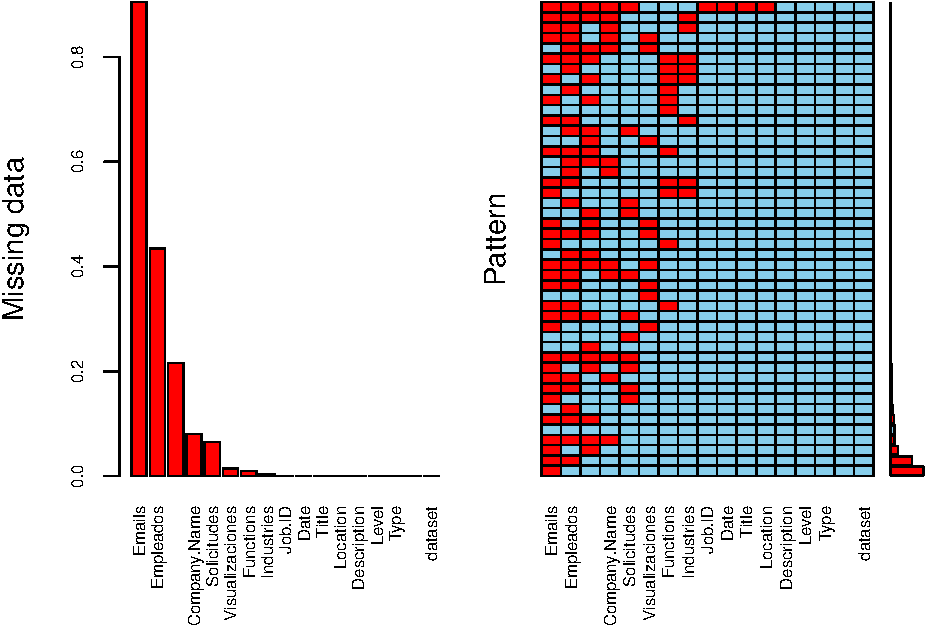
\includegraphics{data_cleaning_files/figure-latex/unnamed-chunk-14-1.pdf}

\begin{verbatim}
## 
##  Variables sorted by number of missings: 
##            Variable        Count
##              Emails 0.9048248513
##           Empleados 0.4339061467
##  Recommended.Flavor 0.2154659617
##        Company.Name 0.0799735625
##         Solicitudes 0.0654329147
##     Visualizaciones 0.0148711170
##           Functions 0.0099140780
##          Industries 0.0039656312
##              Job.ID 0.0003304693
##                Date 0.0003304693
##               Title 0.0003304693
##            Location 0.0003304693
##         Description 0.0000000000
##               Level 0.0000000000
##                Type 0.0000000000
##   Quick.Application 0.0000000000
##             dataset 0.0000000000
\end{verbatim}

Tratamos los valores perdidos numéricos sustituyéndolos por la mediana.

\begin{Shaded}
\begin{Highlighting}[]
\NormalTok{jobs \textless{}{-}}\StringTok{ }\NormalTok{jobs }\OperatorTok{\%\textgreater{}\%}
\StringTok{  }\KeywordTok{group\_by}\NormalTok{(Level, Quick.Application) }\OperatorTok{\%\textgreater{}\%}
\StringTok{    }\KeywordTok{mutate}\NormalTok{(}\DataTypeTok{Solicitudes =} \KeywordTok{ifelse}\NormalTok{(}\KeywordTok{is.na}\NormalTok{(Solicitudes), }\KeywordTok{median}\NormalTok{(Solicitudes, }\DataTypeTok{na.rm =} \OtherTok{TRUE}\NormalTok{), Solicitudes))}
\NormalTok{jobs \textless{}{-}}\StringTok{ }\NormalTok{jobs }\OperatorTok{\%\textgreater{}\%}
\StringTok{  }\KeywordTok{group\_by}\NormalTok{(Level, Quick.Application) }\OperatorTok{\%\textgreater{}\%}
\StringTok{    }\KeywordTok{mutate}\NormalTok{(}\DataTypeTok{Visualizaciones =} \KeywordTok{ifelse}\NormalTok{(}\KeywordTok{is.na}\NormalTok{(Visualizaciones), }\KeywordTok{median}\NormalTok{(Visualizaciones, }\DataTypeTok{na.rm =} \OtherTok{TRUE}\NormalTok{), Visualizaciones))}
\end{Highlighting}
\end{Shaded}

Comprobamos cómo queda ahora la distribución de valores perdidos.

\begin{Shaded}
\begin{Highlighting}[]
\KeywordTok{sum}\NormalTok{(}\KeywordTok{is.na}\NormalTok{(jobs))}
\end{Highlighting}
\end{Shaded}

\begin{verbatim}
## [1] 4991
\end{verbatim}

\begin{Shaded}
\begin{Highlighting}[]
\KeywordTok{aggr}\NormalTok{(jobs, }\DataTypeTok{numbers=}\OtherTok{TRUE}\NormalTok{, }\DataTypeTok{sortVars=}\OtherTok{TRUE}\NormalTok{, }\DataTypeTok{labels=}\KeywordTok{names}\NormalTok{(jobs),}
\DataTypeTok{cex.axis=}\NormalTok{.}\DecValTok{7}\NormalTok{, }\DataTypeTok{gap=}\DecValTok{3}\NormalTok{, }\DataTypeTok{ylab=}\KeywordTok{c}\NormalTok{(}\StringTok{"Missing data"}\NormalTok{,}\StringTok{"Pattern"}\NormalTok{))}
\end{Highlighting}
\end{Shaded}

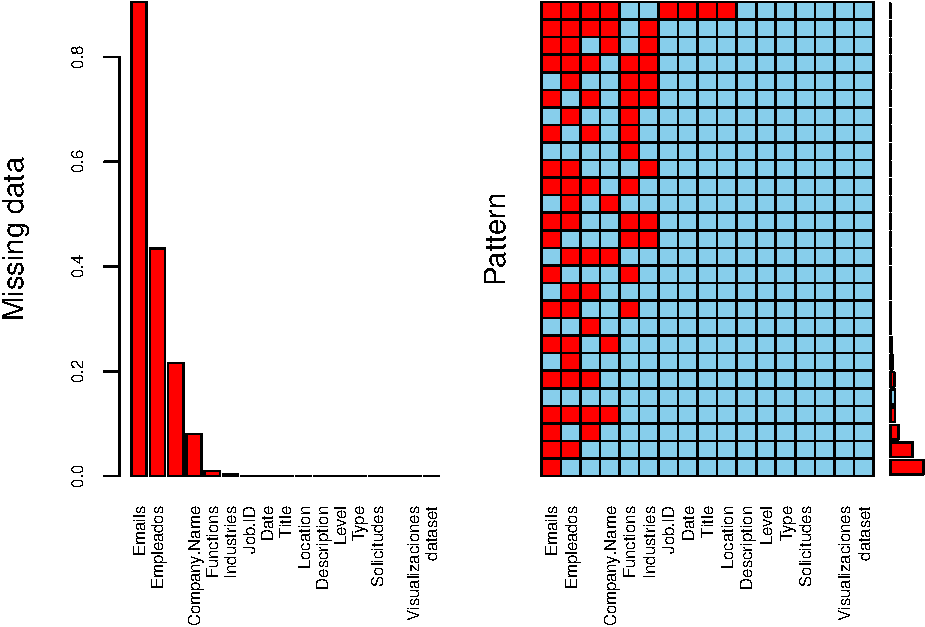
\includegraphics{data_cleaning_files/figure-latex/unnamed-chunk-16-1.pdf}

\begin{verbatim}
## 
##  Variables sorted by number of missings: 
##            Variable        Count
##              Emails 0.9048248513
##           Empleados 0.4339061467
##  Recommended.Flavor 0.2154659617
##        Company.Name 0.0799735625
##           Functions 0.0099140780
##          Industries 0.0039656312
##              Job.ID 0.0003304693
##                Date 0.0003304693
##               Title 0.0003304693
##            Location 0.0003304693
##         Description 0.0000000000
##               Level 0.0000000000
##                Type 0.0000000000
##         Solicitudes 0.0000000000
##   Quick.Application 0.0000000000
##     Visualizaciones 0.0000000000
##             dataset 0.0000000000
\end{verbatim}

Los valores perdidos se han reducido bastante y los que quedan se dejan
así porque será importante para posteriores análisis.

\hypertarget{identificacion-y-tratamiento-de-valores-extremos}{%
\subsection{3.2. Identificación y tratamiento de valores
extremos}\label{identificacion-y-tratamiento-de-valores-extremos}}

Empezamos haciendo una visualización sencilla de las variables
susceptibles de tener valores aislados.

\begin{Shaded}
\begin{Highlighting}[]
\KeywordTok{grid.arrange}\NormalTok{(}
  \KeywordTok{qplot}\NormalTok{(Date, }\DataTypeTok{data=}\NormalTok{jobs)}\OperatorTok{+}\StringTok{ }\KeywordTok{theme}\NormalTok{(}\DataTypeTok{axis.text.x =} \KeywordTok{element\_text}\NormalTok{(}\DataTypeTok{angle =} \DecValTok{25}\NormalTok{)),}
  \KeywordTok{qplot}\NormalTok{(Level, }\DataTypeTok{data=}\NormalTok{jobs)}\OperatorTok{+}\StringTok{ }\KeywordTok{theme}\NormalTok{(}\DataTypeTok{axis.text.x =} \KeywordTok{element\_text}\NormalTok{(}\DataTypeTok{angle =} \DecValTok{20}\NormalTok{, }\DataTypeTok{hjust=}\FloatTok{0.7}\NormalTok{, }\DataTypeTok{size =} \DecValTok{7}\NormalTok{)),}
  \KeywordTok{qplot}\NormalTok{(Type, }\DataTypeTok{data=}\NormalTok{jobs)}\OperatorTok{+}\StringTok{ }\KeywordTok{theme}\NormalTok{(}\DataTypeTok{axis.text.x =} \KeywordTok{element\_text}\NormalTok{(}\DataTypeTok{angle =} \DecValTok{20}\NormalTok{, }\DataTypeTok{hjust=}\DecValTok{1}\NormalTok{)),}
  \KeywordTok{qplot}\NormalTok{(Solicitudes, }\DataTypeTok{data=}\NormalTok{jobs)}\OperatorTok{+}\StringTok{ }\KeywordTok{theme}\NormalTok{(}\DataTypeTok{axis.text.x =} \KeywordTok{element\_text}\NormalTok{(}\DataTypeTok{angle =} \DecValTok{25}\NormalTok{)),}
  \KeywordTok{qplot}\NormalTok{(Empleados, }\DataTypeTok{data=}\NormalTok{jobs)}\OperatorTok{+}\StringTok{ }\KeywordTok{theme}\NormalTok{(}\DataTypeTok{axis.text.x =} \KeywordTok{element\_text}\NormalTok{(}\DataTypeTok{angle =} \DecValTok{30}\NormalTok{, }\DataTypeTok{hjust=}\FloatTok{0.7}\NormalTok{, }\DataTypeTok{size =} \DecValTok{7}\NormalTok{)),}
  \KeywordTok{qplot}\NormalTok{(Visualizaciones, }\DataTypeTok{data=}\NormalTok{jobs)}\OperatorTok{+}\StringTok{ }\KeywordTok{theme}\NormalTok{(}\DataTypeTok{axis.text.x =} \KeywordTok{element\_text}\NormalTok{(}\DataTypeTok{angle =} \DecValTok{25}\NormalTok{)),}
  \KeywordTok{qplot}\NormalTok{(Recommended.Flavor, }\DataTypeTok{data=}\NormalTok{jobs)}\OperatorTok{+}\StringTok{ }\KeywordTok{theme}\NormalTok{(}\DataTypeTok{axis.text.x =} \KeywordTok{element\_text}\NormalTok{(}\DataTypeTok{angle =} \DecValTok{30}\NormalTok{, }\DataTypeTok{hjust=}\FloatTok{0.7}\NormalTok{, }\DataTypeTok{size =} \DecValTok{7}\NormalTok{))}
\NormalTok{)}
\end{Highlighting}
\end{Shaded}

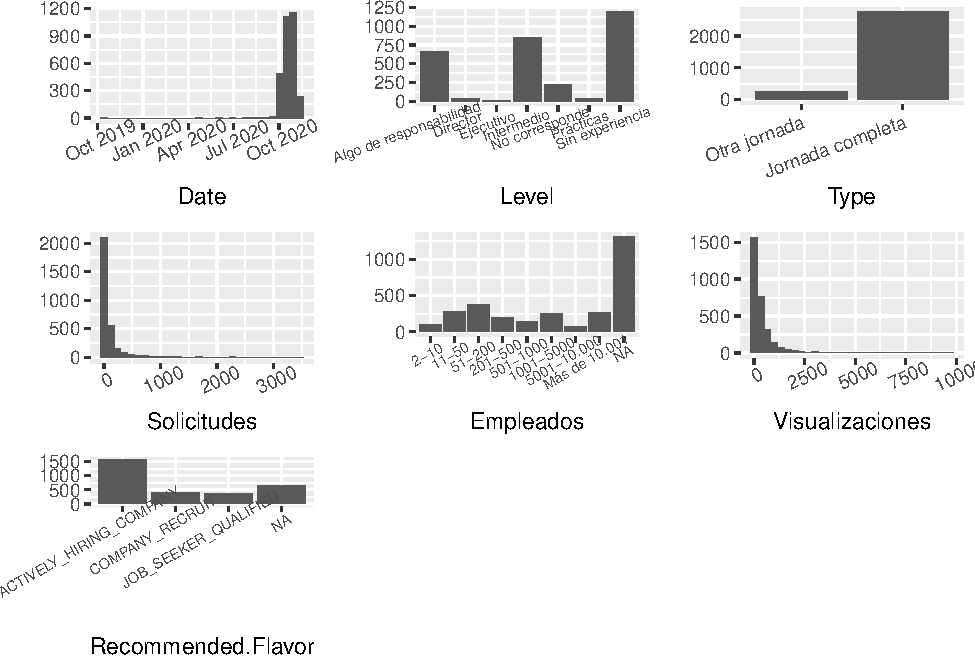
\includegraphics{data_cleaning_files/figure-latex/unnamed-chunk-17-1.pdf}

Hacemos un boxplot para cada una de las variables numéricas agrupándolas
en función de la variable ``Level'' para así visualizar mejor los
valores numéricos.

\begin{Shaded}
\begin{Highlighting}[]
\KeywordTok{ggplot}\NormalTok{(jobs, }\KeywordTok{aes}\NormalTok{(}\DataTypeTok{x=}\NormalTok{Level, }\DataTypeTok{y=}\NormalTok{Solicitudes, }\DataTypeTok{color=}\NormalTok{Level)) }\OperatorTok{+}\StringTok{ }
\StringTok{  }\KeywordTok{ggtitle}\NormalTok{(}\StringTok{"Diagrama de cajas de Solicitudes"}\NormalTok{) }\OperatorTok{+}\StringTok{ }
\StringTok{  }\KeywordTok{scale\_color\_brewer}\NormalTok{(}\DataTypeTok{palette=}\StringTok{"Dark2"}\NormalTok{) }\OperatorTok{+}
\StringTok{  }\KeywordTok{geom\_boxplot}\NormalTok{() }\OperatorTok{+}
\StringTok{  }\KeywordTok{theme}\NormalTok{(}\DataTypeTok{legend.position =} \StringTok{"null"}\NormalTok{) }\OperatorTok{+}
\StringTok{  }\KeywordTok{geom\_jitter}\NormalTok{(}\DataTypeTok{width =} \FloatTok{0.1}\NormalTok{)}
\end{Highlighting}
\end{Shaded}

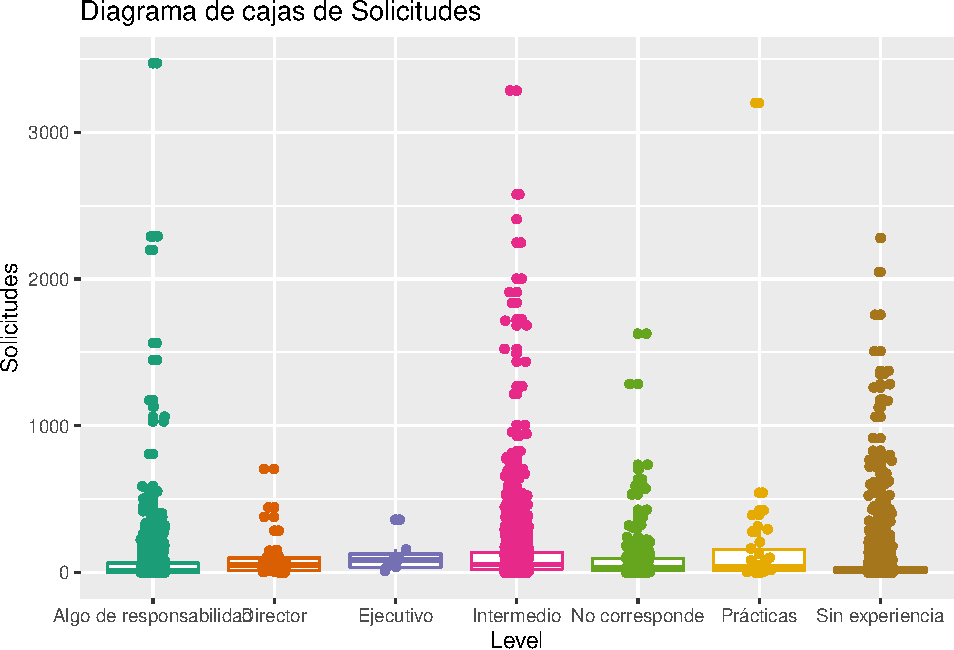
\includegraphics{data_cleaning_files/figure-latex/unnamed-chunk-18-1.pdf}

\begin{Shaded}
\begin{Highlighting}[]
\KeywordTok{ggplot}\NormalTok{(jobs, }\KeywordTok{aes}\NormalTok{(}\DataTypeTok{x=}\NormalTok{Level, }\DataTypeTok{y=}\NormalTok{Visualizaciones, }\DataTypeTok{color=}\NormalTok{Level)) }\OperatorTok{+}\StringTok{ }
\StringTok{  }\KeywordTok{ggtitle}\NormalTok{(}\StringTok{"Diagrama de cajas de Visualizaciones"}\NormalTok{) }\OperatorTok{+}\StringTok{ }
\StringTok{  }\KeywordTok{scale\_color\_brewer}\NormalTok{(}\DataTypeTok{palette=}\StringTok{"Dark2"}\NormalTok{) }\OperatorTok{+}
\StringTok{  }\KeywordTok{geom\_boxplot}\NormalTok{() }\OperatorTok{+}
\StringTok{  }\KeywordTok{theme}\NormalTok{(}\DataTypeTok{legend.position =} \StringTok{"null"}\NormalTok{) }\OperatorTok{+}
\StringTok{  }\KeywordTok{geom\_jitter}\NormalTok{(}\DataTypeTok{width =} \FloatTok{0.1}\NormalTok{)}
\end{Highlighting}
\end{Shaded}

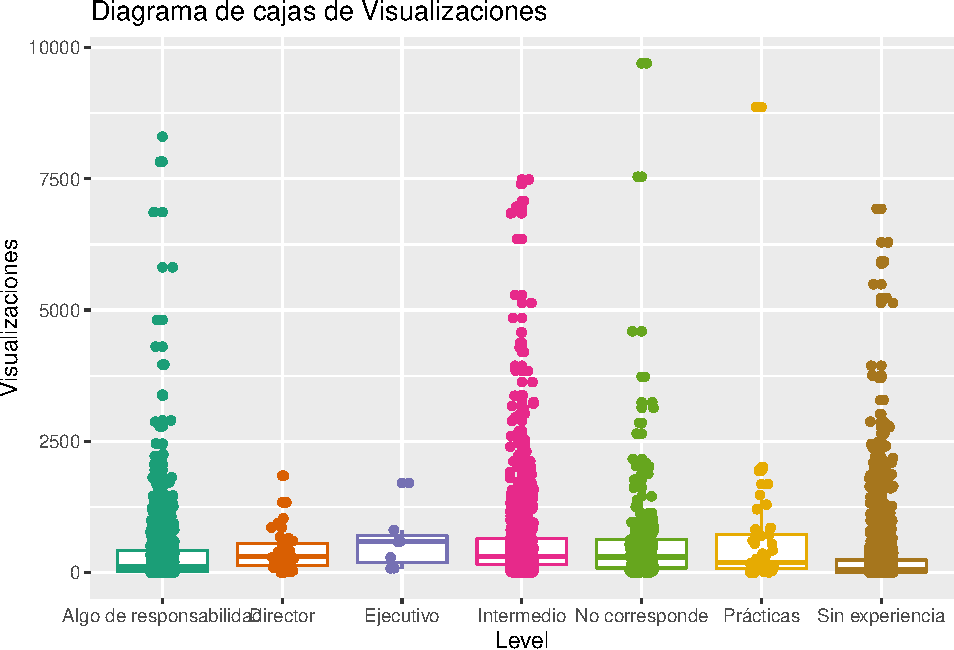
\includegraphics{data_cleaning_files/figure-latex/unnamed-chunk-18-2.pdf}

Como ya se veía por las gráficas anteriores son datos con colas muy
largas a la derecha y algunos de los valores bastante aislados.

Vamos a mirar los 5 valores más aislados de la variable ``Solicitudes''.

\begin{Shaded}
\begin{Highlighting}[]
\KeywordTok{tail}\NormalTok{(}\KeywordTok{sort}\NormalTok{(}\KeywordTok{boxplot.stats}\NormalTok{(jobs}\OperatorTok{$}\NormalTok{Solicitudes)}\OperatorTok{$}\NormalTok{out),}\DecValTok{5}\NormalTok{)}
\end{Highlighting}
\end{Shaded}

\begin{verbatim}
## [1] 2408 2578 3200 3284 3470
\end{verbatim}

Vamos a observar las tres ofertas de trabajo que superan las 3000
solicitudes.

\begin{Shaded}
\begin{Highlighting}[]
\NormalTok{jobs[}\KeywordTok{which}\NormalTok{(jobs}\OperatorTok{$}\NormalTok{Solicitudes }\OperatorTok{\%in\%}\StringTok{ }\KeywordTok{tail}\NormalTok{(}\KeywordTok{sort}\NormalTok{(}\KeywordTok{boxplot.stats}\NormalTok{(jobs}\OperatorTok{$}\NormalTok{Solicitudes)}\OperatorTok{$}\NormalTok{out),}\DecValTok{3}\NormalTok{)),]}
\end{Highlighting}
\end{Shaded}

\begin{verbatim}
## # A tibble: 3 x 17
## # Groups:   Level, Quick.Application [3]
##   Job.ID Date       Company.Name Title Location Description Level Type 
##   <chr>  <date>     <chr>        <chr> <chr>    <chr>       <fct> <fct>
## 1 19527~ 2020-10-27 TouchPal     Data~ San Fra~ About the ~ Algo~ Jorn~
## 2 20047~ 2020-10-25 atisfy       Data~ Hyderab~ The ideal ~ Inte~ Jorn~
## 3 21857~ 2020-10-15 LinkedIn     Data~ Sunnyva~ Data Scien~ Prác~ Otra~
## # ... with 9 more variables: Functions <chr>, Industries <chr>,
## #   Solicitudes <dbl>, Empleados <fct>, Quick.Application <fct>, Emails <chr>,
## #   Visualizaciones <dbl>, Recommended.Flavor <fct>, dataset <fct>
\end{verbatim}

Aunque sean valores extremos, observándolos en detalles parecen
razonables y correctos así que los dejamos.

\hypertarget{analisis-de-los-datos.}{%
\section{4. Análisis de los datos.}\label{analisis-de-los-datos.}}

\hypertarget{selecciuxf3n-de-los-grupos-de-datos-que-se-quieren-analizarcomparar-planificaciuxf3n-de-los-anuxe1lisis-a-aplicar}{%
\subsection{4.1. Selección de los grupos de datos que se quieren
analizar/comparar (planificación de los análisis a
aplicar)}\label{selecciuxf3n-de-los-grupos-de-datos-que-se-quieren-analizarcomparar-planificaciuxf3n-de-los-anuxe1lisis-a-aplicar}}

Para este apartado se realizaran los análsis sobre el dataframe
``jobs''. Se ha preferido mantener por separado dos dataframes ya que,
de eliminar duplicados al mezclar los distintos archivos con sus
localizaciones no se realizaría una correcta visualización.

El dataframe ``jobs'' es el que ha sido limpiado y manipulado
previamente para poder realizar los análisis. En primer lugar será
necesario encontrar la latitud y la longitud de cada una de las
localizaciones. Esto será importante para evaluar posteriormente
correlaciones entre variables y aplicar dos tipos de regresión (lineal y
logística).

Una vez se obtengan esas nuevas variables para la latitud y la longitud
y se comprueben las condiciones de normalidad y homogeneidad se pasará a
realizar una correlación de variables para entender dónde podríamos
aplicar las regresiones.

El modelo de regresión lineal pretenderá predecir el número de
solicitudes respecto a la latitud, longitud y número de visualizaciones.
Por otro lado, el modelo de regresión logística viene a predecir si se
trata de la oferta cuenta con un enlace de solicitud rápida respecto al
nivel de la oferta, el tipo de oferta, el número de solicitudes, el
número de visualizaciones y la variable de tipo de ofertante.

\hypertarget{preparaciuxf3n-de-los-datos-de-longitud-y-latitud.}{%
\subsubsection{4.1.1 Preparación de los datos de Longitud y
Latitud.}\label{preparaciuxf3n-de-los-datos-de-longitud-y-latitud.}}

En primer lugar se obtienen las dos nuevas variables haciendo uso de la
API de OpenStreetMap. Se tienen en cuenta tan sólo estos dos valores
aunque podríamos haber conseguido muchos más datos sobre una
localización más precisa (ésto valdría para hacer análisis por
localidades donde encontrar piso cercano al mayor número de puestos de
trabajo por ejemplo).

\begin{Shaded}
\begin{Highlighting}[]
\NormalTok{jobs}\OperatorTok{$}\NormalTok{Location \textless{}{-}}\StringTok{ }\KeywordTok{str\_remove}\NormalTok{(jobs}\OperatorTok{$}\NormalTok{Location, }\StringTok{"\^{}*y alrededores.*$"}\NormalTok{)}
\NormalTok{jobs}\OperatorTok{$}\NormalTok{Location[}\KeywordTok{which}\NormalTok{(jobs}\OperatorTok{$}\NormalTok{Location }\OperatorTok{==}\StringTok{ "Greater Barcelona Metropolitan Area"}\NormalTok{)] \textless{}{-}}\StringTok{ "Barcelona"}
\NormalTok{jobs}\OperatorTok{$}\NormalTok{Location[}\KeywordTok{which}\NormalTok{(jobs}\OperatorTok{$}\NormalTok{Location }\OperatorTok{==}\StringTok{ "Cracow, Lesser Poland District, Poland"}\NormalTok{)] \textless{}{-}}\StringTok{ "Cracow, Poland"}
\NormalTok{jobs}\OperatorTok{$}\NormalTok{Location[}\KeywordTok{which}\NormalTok{(jobs}\OperatorTok{$}\NormalTok{Location }\OperatorTok{==}\StringTok{ "New York City Metropolitan Area"}\NormalTok{)] \textless{}{-}}\StringTok{ "New York"}
\NormalTok{jobs}\OperatorTok{$}\NormalTok{Location[}\KeywordTok{which}\NormalTok{(jobs}\OperatorTok{$}\NormalTok{Location }\OperatorTok{==}\StringTok{ "Hong Kong, Hong Kong SAR"}\NormalTok{)] \textless{}{-}}\StringTok{ "Hong Kong"}
\NormalTok{jobs}\OperatorTok{$}\NormalTok{Location[}\KeywordTok{which}\NormalTok{(jobs}\OperatorTok{$}\NormalTok{Location }\OperatorTok{==}\StringTok{ "Burnaby (Maywood / Marlborough / Oakalla / Windsor), V5H, CA"}\NormalTok{)] \textless{}{-}}\StringTok{ "Burnaby"}
\NormalTok{jobs}\OperatorTok{$}\NormalTok{Location[}\KeywordTok{which}\NormalTok{(jobs}\OperatorTok{$}\NormalTok{Location }\OperatorTok{==}\StringTok{ "District Brno{-}City, Czech Republic"}\NormalTok{)] \textless{}{-}}\StringTok{ "Czech Republic"}
\NormalTok{jobs}\OperatorTok{$}\NormalTok{Location[}\KeywordTok{which}\NormalTok{(jobs}\OperatorTok{$}\NormalTok{Location }\OperatorTok{==}\StringTok{ "Silkeborg, Middle Jutland, Denmark"}\NormalTok{)] \textless{}{-}}\StringTok{ "Denmark"}
\NormalTok{jobs}\OperatorTok{$}\NormalTok{Location[}\KeywordTok{which}\NormalTok{(jobs}\OperatorTok{$}\NormalTok{Location }\OperatorTok{==}\StringTok{ "Prague, The Capital, Czech Republic"}\NormalTok{)] \textless{}{-}}\StringTok{ "Prague"}
\NormalTok{jobs}\OperatorTok{$}\NormalTok{Location[}\KeywordTok{which}\NormalTok{(jobs}\OperatorTok{$}\NormalTok{Location }\OperatorTok{==}\StringTok{ "Kuala Lumpur, Federal Territory of Kuala Lumpur, Malaysia"}\NormalTok{)] \textless{}{-}}\StringTok{ "Malaysia"}
\NormalTok{jobs}\OperatorTok{$}\NormalTok{Location[}\KeywordTok{which}\NormalTok{(jobs}\OperatorTok{$}\NormalTok{Location }\OperatorTok{==}\StringTok{ "Genève et périphérie"}\NormalTok{)] \textless{}{-}}\StringTok{ "Genève"}
\NormalTok{jobs}\OperatorTok{$}\NormalTok{Location[}\KeywordTok{which}\NormalTok{(jobs}\OperatorTok{$}\NormalTok{Location }\OperatorTok{==}\StringTok{ "Dallas{-}Fort Worth Metroplex"}\NormalTok{)] \textless{}{-}}\StringTok{ "Dallas"}
\NormalTok{jobs}\OperatorTok{$}\NormalTok{Location[}\KeywordTok{which}\NormalTok{(jobs}\OperatorTok{$}\NormalTok{Location }\OperatorTok{==}\StringTok{ "Raleigh{-}Durham{-}Chapel Hill Area"}\NormalTok{)] \textless{}{-}}\StringTok{ "Raleigh"}
\NormalTok{jobs}\OperatorTok{$}\NormalTok{Location[}\KeywordTok{which}\NormalTok{(jobs}\OperatorTok{$}\NormalTok{Location }\OperatorTok{==}\StringTok{ "Herzliyya, Tel Aviv, Israel"}\NormalTok{)] \textless{}{-}}\StringTok{ "Herzliya"}
\NormalTok{jobs}\OperatorTok{$}\NormalTok{Location[}\KeywordTok{which}\NormalTok{(jobs}\OperatorTok{$}\NormalTok{Location }\OperatorTok{==}\StringTok{ "New Territories, Hong Kong SAR"}\NormalTok{)] \textless{}{-}}\StringTok{ "Hong Kong"}
\NormalTok{jobs}\OperatorTok{$}\NormalTok{Location[}\KeywordTok{which}\NormalTok{(jobs}\OperatorTok{$}\NormalTok{Location }\OperatorTok{==}\StringTok{ "Des Moines Metropolitan Area"}\NormalTok{)] \textless{}{-}}\StringTok{ "Des Moines"}
\NormalTok{jobs}\OperatorTok{$}\NormalTok{Location[}\KeywordTok{which}\NormalTok{(jobs}\OperatorTok{$}\NormalTok{Location }\OperatorTok{==}\StringTok{ "Greater Minneapolis{-}St. Paul Area"}\NormalTok{)] \textless{}{-}}\StringTok{ "Minneapolis"}
\NormalTok{jobs}\OperatorTok{$}\NormalTok{Location[}\KeywordTok{which}\NormalTok{(jobs}\OperatorTok{$}\NormalTok{Location }\OperatorTok{==}\StringTok{ "Greater Munich Metropolitan Area"}\NormalTok{)] \textless{}{-}}\StringTok{ "Munich"}
\NormalTok{jobs}\OperatorTok{$}\NormalTok{Location[}\KeywordTok{which}\NormalTok{(jobs}\OperatorTok{$}\NormalTok{Location }\OperatorTok{==}\StringTok{ "Gurgaon Sub{-}District, Haryana, India"}\NormalTok{)] \textless{}{-}}\StringTok{ "Gurgaon"}
\NormalTok{jobs}\OperatorTok{$}\NormalTok{Location[}\KeywordTok{which}\NormalTok{(jobs}\OperatorTok{$}\NormalTok{Location }\OperatorTok{==}\StringTok{ "Village of Mayfield, OH, US"}\NormalTok{)] \textless{}{-}}\StringTok{ "Cleveland"}
\NormalTok{jobs}\OperatorTok{$}\NormalTok{Location[}\KeywordTok{which}\NormalTok{(jobs}\OperatorTok{$}\NormalTok{Location }\OperatorTok{==}\StringTok{ "Kraków i okolice"}\NormalTok{)] \textless{}{-}}\StringTok{ "Kraków"}

\NormalTok{jobs\_with\_duplicates}\OperatorTok{$}\NormalTok{Location \textless{}{-}}\StringTok{ }\KeywordTok{str\_remove}\NormalTok{(jobs\_with\_duplicates}\OperatorTok{$}\NormalTok{Location, }\StringTok{"\^{}*y alrededores.*$"}\NormalTok{)}
\NormalTok{jobs\_with\_duplicates}\OperatorTok{$}\NormalTok{Location[}\KeywordTok{which}\NormalTok{(jobs\_with\_duplicates}\OperatorTok{$}\NormalTok{Location }\OperatorTok{==}\StringTok{ "Greater Barcelona Metropolitan Area"}\NormalTok{)] \textless{}{-}}\StringTok{ "Barcelona"}
\NormalTok{jobs\_with\_duplicates}\OperatorTok{$}\NormalTok{Location[}\KeywordTok{which}\NormalTok{(jobs\_with\_duplicates}\OperatorTok{$}\NormalTok{Location }\OperatorTok{==}\StringTok{ "Cracow, Lesser Poland District, Poland"}\NormalTok{)] \textless{}{-}}\StringTok{ "Cracow, Poland"}
\NormalTok{jobs\_with\_duplicates}\OperatorTok{$}\NormalTok{Location[}\KeywordTok{which}\NormalTok{(jobs\_with\_duplicates}\OperatorTok{$}\NormalTok{Location }\OperatorTok{==}\StringTok{ "New York City Metropolitan Area"}\NormalTok{)] \textless{}{-}}\StringTok{ "New York"}
\NormalTok{jobs\_with\_duplicates}\OperatorTok{$}\NormalTok{Location[}\KeywordTok{which}\NormalTok{(jobs\_with\_duplicates}\OperatorTok{$}\NormalTok{Location }\OperatorTok{==}\StringTok{ "Hong Kong, Hong Kong SAR"}\NormalTok{)] \textless{}{-}}\StringTok{ "Hong Kong"}
\NormalTok{jobs\_with\_duplicates}\OperatorTok{$}\NormalTok{Location[}\KeywordTok{which}\NormalTok{(jobs\_with\_duplicates}\OperatorTok{$}\NormalTok{Location }\OperatorTok{==}\StringTok{ "Burnaby (Maywood / Marlborough / Oakalla / Windsor), V5H, CA"}\NormalTok{)] \textless{}{-}}\StringTok{ "Burnaby"}
\NormalTok{jobs\_with\_duplicates}\OperatorTok{$}\NormalTok{Location[}\KeywordTok{which}\NormalTok{(jobs\_with\_duplicates}\OperatorTok{$}\NormalTok{Location }\OperatorTok{==}\StringTok{ "District Brno{-}City, Czech Republic"}\NormalTok{)] \textless{}{-}}\StringTok{ "Czech Republic"}
\NormalTok{jobs\_with\_duplicates}\OperatorTok{$}\NormalTok{Location[}\KeywordTok{which}\NormalTok{(jobs\_with\_duplicates}\OperatorTok{$}\NormalTok{Location }\OperatorTok{==}\StringTok{ "Silkeborg, Middle Jutland, Denmark"}\NormalTok{)] \textless{}{-}}\StringTok{ "Denmark"}
\NormalTok{jobs\_with\_duplicates}\OperatorTok{$}\NormalTok{Location[}\KeywordTok{which}\NormalTok{(jobs\_with\_duplicates}\OperatorTok{$}\NormalTok{Location }\OperatorTok{==}\StringTok{ "Prague, The Capital, Czech Republic"}\NormalTok{)] \textless{}{-}}\StringTok{ "Prague"}
\NormalTok{jobs\_with\_duplicates}\OperatorTok{$}\NormalTok{Location[}\KeywordTok{which}\NormalTok{(jobs\_with\_duplicates}\OperatorTok{$}\NormalTok{Location }\OperatorTok{==}\StringTok{ "Kuala Lumpur, Federal Territory of Kuala Lumpur, Malaysia"}\NormalTok{)] \textless{}{-}}\StringTok{ "Malaysia"}
\NormalTok{jobs\_with\_duplicates}\OperatorTok{$}\NormalTok{Location[}\KeywordTok{which}\NormalTok{(jobs\_with\_duplicates}\OperatorTok{$}\NormalTok{Location }\OperatorTok{==}\StringTok{ "Genève et périphérie"}\NormalTok{)] \textless{}{-}}\StringTok{ "Genève"}
\NormalTok{jobs\_with\_duplicates}\OperatorTok{$}\NormalTok{Location[}\KeywordTok{which}\NormalTok{(jobs\_with\_duplicates}\OperatorTok{$}\NormalTok{Location }\OperatorTok{==}\StringTok{ "Dallas{-}Fort Worth Metroplex"}\NormalTok{)] \textless{}{-}}\StringTok{ "Dallas"}
\NormalTok{jobs\_with\_duplicates}\OperatorTok{$}\NormalTok{Location[}\KeywordTok{which}\NormalTok{(jobs\_with\_duplicates}\OperatorTok{$}\NormalTok{Location }\OperatorTok{==}\StringTok{ "Raleigh{-}Durham{-}Chapel Hill Area"}\NormalTok{)] \textless{}{-}}\StringTok{ "Raleigh"}
\NormalTok{jobs\_with\_duplicates}\OperatorTok{$}\NormalTok{Location[}\KeywordTok{which}\NormalTok{(jobs\_with\_duplicates}\OperatorTok{$}\NormalTok{Location }\OperatorTok{==}\StringTok{ "Herzliyya, Tel Aviv, Israel"}\NormalTok{)] \textless{}{-}}\StringTok{ "Herzliya"}
\NormalTok{jobs\_with\_duplicates}\OperatorTok{$}\NormalTok{Location[}\KeywordTok{which}\NormalTok{(jobs\_with\_duplicates}\OperatorTok{$}\NormalTok{Location }\OperatorTok{==}\StringTok{ "New Territories, Hong Kong SAR"}\NormalTok{)] \textless{}{-}}\StringTok{ "Hong Kong"}
\NormalTok{jobs\_with\_duplicates}\OperatorTok{$}\NormalTok{Location[}\KeywordTok{which}\NormalTok{(jobs\_with\_duplicates}\OperatorTok{$}\NormalTok{Location }\OperatorTok{==}\StringTok{ "Des Moines Metropolitan Area"}\NormalTok{)] \textless{}{-}}\StringTok{ "Des Moines"}
\NormalTok{jobs\_with\_duplicates}\OperatorTok{$}\NormalTok{Location[}\KeywordTok{which}\NormalTok{(jobs\_with\_duplicates}\OperatorTok{$}\NormalTok{Location }\OperatorTok{==}\StringTok{ "Greater Minneapolis{-}St. Paul Area"}\NormalTok{)] \textless{}{-}}\StringTok{ "Minneapolis"}
\NormalTok{jobs\_with\_duplicates}\OperatorTok{$}\NormalTok{Location[}\KeywordTok{which}\NormalTok{(jobs\_with\_duplicates}\OperatorTok{$}\NormalTok{Location }\OperatorTok{==}\StringTok{ "Greater Munich Metropolitan Area"}\NormalTok{)] \textless{}{-}}\StringTok{ "Munich"}
\NormalTok{jobs\_with\_duplicates}\OperatorTok{$}\NormalTok{Location[}\KeywordTok{which}\NormalTok{(jobs\_with\_duplicates}\OperatorTok{$}\NormalTok{Location }\OperatorTok{==}\StringTok{ "Gurgaon Sub{-}District, Haryana, India"}\NormalTok{)] \textless{}{-}}\StringTok{ "Gurgaon"}
\NormalTok{jobs\_with\_duplicates}\OperatorTok{$}\NormalTok{Location[}\KeywordTok{which}\NormalTok{(jobs\_with\_duplicates}\OperatorTok{$}\NormalTok{Location }\OperatorTok{==}\StringTok{ "Village of Mayfield, OH, US"}\NormalTok{)] \textless{}{-}}\StringTok{ "Cleveland"}
\NormalTok{jobs\_with\_duplicates}\OperatorTok{$}\NormalTok{Location[}\KeywordTok{which}\NormalTok{(jobs\_with\_duplicates}\OperatorTok{$}\NormalTok{Location }\OperatorTok{==}\StringTok{ "Kraków i okolice"}\NormalTok{)] \textless{}{-}}\StringTok{ "Kraków"}

\NormalTok{OSM\_jobs \textless{}{-}}\StringTok{ }\KeywordTok{geocode\_OSM}\NormalTok{(jobs}\OperatorTok{$}\NormalTok{Location, }\DataTypeTok{details =} \OtherTok{TRUE}\NormalTok{, }\DataTypeTok{as.data.frame =} \OtherTok{TRUE}\NormalTok{)}
\NormalTok{jobs\_merged\textless{}{-}}\KeywordTok{merge}\NormalTok{(}\DataTypeTok{x=}\NormalTok{jobs,}\DataTypeTok{y=}\NormalTok{OSM\_jobs[}\DecValTok{2}\OperatorTok{:}\DecValTok{3}\NormalTok{], }\DataTypeTok{by =} \DecValTok{0}\NormalTok{, }\DataTypeTok{all=} \OtherTok{TRUE}\NormalTok{)}

\KeywordTok{write.csv}\NormalTok{(jobs\_merged,}\StringTok{"jobs\_merged.csv"}\NormalTok{)}

\NormalTok{OSM\_jobs\_duplicates \textless{}{-}}\StringTok{ }\KeywordTok{geocode\_OSM}\NormalTok{(jobs\_with\_duplicates}\OperatorTok{$}\NormalTok{Location, }\DataTypeTok{details =} \OtherTok{TRUE}\NormalTok{, }\DataTypeTok{as.data.frame =} \OtherTok{TRUE}\NormalTok{)}
\NormalTok{jobs\_merged\_with\_duplicates\textless{}{-}}\KeywordTok{merge}\NormalTok{(}\DataTypeTok{x=}\NormalTok{jobs\_with\_duplicates,}\DataTypeTok{y=}\NormalTok{OSM\_jobs\_duplicates[}\DecValTok{2}\OperatorTok{:}\DecValTok{3}\NormalTok{], }\DataTypeTok{by =} \DecValTok{0}\NormalTok{, }\DataTypeTok{all=} \OtherTok{TRUE}\NormalTok{)}

\KeywordTok{write.csv}\NormalTok{(jobs\_merged\_with\_duplicates,}\StringTok{"jobs\_merged\_with\_duplicates.csv"}\NormalTok{)}

\KeywordTok{head}\NormalTok{(OSM\_jobs)}
\end{Highlighting}
\end{Shaded}

\begin{verbatim}
##                                 query      lat       lon  lat_min  lat_max
## 1 Edinburgh, Scotland, United Kingdom 55.95335 -3.188375 55.81879 56.00408
## 2 Edinburgh, Scotland, United Kingdom 55.95335 -3.188375 55.81879 56.00408
## 3  Aberdeen, Scotland, United Kingdom 57.14824 -2.092809 57.07619 57.23531
## 4                         Glasgow, GB 55.86098 -4.248879 55.70098 56.02098
## 5                         Glasgow, GB 55.86098 -4.248879 55.70098 56.02098
## 6                         Glasgow, GB 55.86098 -4.248879 55.70098 56.02098
##     lon_min   lon_max  place_id osm_type   osm_id place_rank
## 1 -3.449533 -3.074951 257101080 relation  1920901         12
## 2 -3.449533 -3.074951 257101080 relation  1920901         12
## 3 -2.360940 -2.016151 257105109 relation  1900654         12
## 4 -4.408879 -4.088879    107701     node 11127374         16
## 5 -4.408879 -4.088879    107701     node 11127374         16
## 6 -4.408879 -4.088879    107701     node 11127374         16
##                                              display_name    class
## 1             City of Edinburgh, Scotland, United Kingdom boundary
## 2             City of Edinburgh, Scotland, United Kingdom boundary
## 3                 Aberdeen City, Scotland, United Kingdom boundary
## 4 Glasgow, Glasgow City, Scotland, G2 9SD, United Kingdom    place
## 5 Glasgow, Glasgow City, Scotland, G2 9SD, United Kingdom    place
## 6 Glasgow, Glasgow City, Scotland, G2 9SD, United Kingdom    place
##             type       importance
## 1 administrative  1.0867042570635
## 2 administrative  1.0867042570635
## 3 administrative  1.0099117188774
## 4           city 0.79905249303697
## 5           city 0.79905249303697
## 6           city 0.79905249303697
##                                                                                    icon
## 1 https://nominatim.openstreetmap.org/ui/mapicons//poi_boundary_administrative.p.20.png
## 2 https://nominatim.openstreetmap.org/ui/mapicons//poi_boundary_administrative.p.20.png
## 3 https://nominatim.openstreetmap.org/ui/mapicons//poi_boundary_administrative.p.20.png
## 4              https://nominatim.openstreetmap.org/ui/mapicons//poi_place_city.p.20.png
## 5              https://nominatim.openstreetmap.org/ui/mapicons//poi_place_city.p.20.png
## 6              https://nominatim.openstreetmap.org/ui/mapicons//poi_place_city.p.20.png
\end{verbatim}

\begin{Shaded}
\begin{Highlighting}[]
\KeywordTok{head}\NormalTok{(jobs\_merged)}
\end{Highlighting}
\end{Shaded}

\begin{verbatim}
##   Row.names     Job.ID       Date               Company.Name
## 1         1 2011662890 2020-10-15                    Dufrain
## 2        10 2249373089 2020-11-05               Accenture UK
## 3       100 2249373063 2020-11-05               Accenture UK
## 4      1000 2187582068 2020-10-16 Opus Recruitment Solutions
## 5      1001 2198827173 2020-10-21               Checkout.com
## 6      1002 2176271964 2020-10-13             Venture Search
##                         Title                            Location
## 1               Data Engineer Edinburgh, Scotland, United Kingdom
## 2 User Researcher - Newcastle                         Glasgow, GB
## 3         Cloud Data Engineer                         Glasgow, GB
## 4              Data Scientist     Oxford, England, United Kingdom
## 5         Lead Data Scientist     London, England, United Kingdom
## 6     Quantitative Researcher     London, England, United Kingdom
##                                                                                                                                                                                                                                                                                                                                                                                                                                                                                                                                                                                                                                                                                                                                                                                                                                                                                                                                                                                                                                                                                                                                                                                                                                                                                                                                                                                                                                                                                                                                                                                                                                                                                                                                                                                                                                                                                                                                                                                                                                                                                                                                                                                                                                                                                                                                                                                                                                                                                                                                                                                                                                                                                                                                                                                                                                                                                                                                                                                                                                                                                                                                                                                                                                                                                                                                                                                                                                                                                                                                                                                                                                                                                                                                                                                                                                                                                                                                                                                                                                                                                                                                                                                                                                                                                                                                                                                                                                                                                                                                                                                                                                                                                                                                                                                                                                                                                                                                                                                                                                                                                                                                                                                                                                                                                                                                                                                                                                                                                                                                                                                                                                                                                                                                                                                                                                                                                                      Description
## 1                                                                                                                                                                                                                                                                                                                                                                                                                                                                                                                                                                                                                                                                                                                                                                                                                                                                                                                                                                                                                                                                                                                                                                                                                                                                                                                                                                                                                                                                                                                                                                                                                                                                                                                                                                                                                                                                                                                                                                                                                                                                                                                                                                                                                                                                                                                                                                                                                                                                                                                                                                                      Data Engineer London, Edinburgh OR Manchester   We are Dufrain. We’re a market-leading Data Management, Analytics and BI consultancy with offices across the UK, working with some of the biggest names in the Financial Services industry. We are proud to be an agile, client focused consultancy where we all share a common goal.  As we continue to build and strengthen our capability, a number of exciting opportunities have arisen to join our market-leading Data Management and Analytics Consultancy. We are looking for dynamic individuals, with proven experience and strong technical skills to join our teams in our Edinburgh, London and Manchester offices.  What we offer you: Working as a Data Engineer at Dufrain you’ll have the opportunity to work with a creative and highly skilled team of consultants who have expertise in technical delivery, technologies and concepts in areas such as Data Storage, Data Ingestion, Data Integration, Data Warehousing, Data Preparation and Cloud Infrastructure. You will also have your own ‘people coach’ to guide and support you with your career journey with us. Dufrain offers an autonomous environment where you have opportunities to have access to training tools & technical community groups and provides multi sector and international client exposure.    Who we’re looking for: we are looking for Data Engineers who have a genuine interest of rich data and have experience on delivery that contributes to wider business outcomes and be able to concisely articulate to stakeholders and interested parties their role and solutions in a way that can be easily understood.   Essential Requirements: Strong cloud engineering experience  Skilled in multiple languages such as SQL, Python, Java, Scala, Julia Hands on experience of cloud platforms such as Azure, AWS & GCP - (Certified to practitioner level in at least one provider) Experience working with one or more of the tools - Spark, Kafka, Snowflake, Hadoop Experience working with both SQL and NoSQL foundational tools and databases such as Cassandra, MongoDB  Experience delivering multiple solutions using key techniques such as Data Modelling, DWH, Lakes, ETL, ELT, Virtualisation & Streaming Solid knowledge of development principles such as ETL, DWH & Streaming  Minimum 2 years’ experience as Data Engineer with previous experience in industry or as SQL developer Flexibility to travel to and work on client sites within the UK and occasionally Europe Excellent track record in executive stakeholder management and maintaining valuable relationships. Takes ownership and accountability for critical initiatives and deliverables both internally and for clients Awareness of current market trends in data having the ability to influence opinion and decisioning across the Data Management spectrum A passionate desire and attitude to learn new tools  What to do next: Please apply via the application link below. Once your application has been received a representative from the Dufrain Recruitment team will review your profile and inform you of the next steps.   Please note: The recruitment process will require any candidates that are shortlisted to complete an online technical assessment.
## 2                                                                                                                                                                                                                                                                                                                                                                                                                                                                                                                                                                                                                                                                                                                                                                                                                                                                                                                                                                                                                                    User Researcher - Newcastle  Location: Newcastle Upon-Tyne  Salary: £28,000 - £48,000  Career Level: (Accenture will be recruiting at the following levels: Senior Analyst, Consultant)  Accenture is a leading global professional services company, providing a broad range of services in strategy and consulting, interactive, technology and operations, with digital capabilities across all of these services. With our thought leadership and culture of innovation, we apply industry expertise, diverse skill sets and next-generation technology to each business challenge.  We believe in inclusion and diversity and supporting the whole person. Our core values comprise of Stewardship, Best People, Client Value Creation, One Global Network, Respect for the Individual and Integrity. Year after year, Accenture is recognized worldwide not just for business performance but for inclusion and diversity too.  “Across the globe, one thing is universally true of the people of Accenture: We care deeply about what we do and the impact we have with our clients and with the communities in which we work and live. It is personal to all of us.” – Julie Sweet, Accenture CEO  As a User Researcher you will work with a team of creative and passionate UX Design specialists who are responsible for creating user-centred designs for digital products and services.  This is a great opportunity to work across multiple different clients in a range of industries. As a member of our close-knit UX and Design team, you will champion the value of User-Centred Design across all products and services as part of delivery best practice.  As a User Researcher, you will:  Plan, design and conduct user research sessions to support the design and development of client services and products  Lead the research process from developing user recruitment briefs through to conducting sessions remotely or face-to-face, session analysis, report writing and playback to your team  Collaborate with product owners and service managers to devise appropriate research strategies that will generate focused insights  Convert concepts and emerging findings into high quality stimulus material  Work closely with designers and developers to turn user data and insights into actionable requirements that feed into prototype development, and influence product direction  Work as a part of Agile delivery teams and possess the hard and soft skills required to participate in design and delivery and be able to identify and progress client issues  Work closely with our UX & Design Team, to share knowledge, learn new skills, and design transformational services    Set yourself apart:  Relevant experience as a User Researcher  You have worked as part of an Agile Scrum team  You are always comfortable advocating for your users, and helping your team and stakeholders navigate a user-centred design process  Some experience working with GDS standards would be beneficial but not essential   What’s In It For You  At Accenture in addition to a competitive basic salary, you will also have an extensive benefits package which includes 30 days’ vacation per year, gym subsidy, private medical insurance and 3 extra days leave per year for charitable work of your choice!  Flexibility and mobility are required to deliver this role as there will be requirements to spend time onsite with our clients and partners to enable delivery of the first-class services we are known for.   About Accenture  Accenture is a leading global professional services company, providing a broad range of services in strategy and consulting, interactive, technology and operations, with digital capabilities across all of these services. We combine unmatched experience and specialized capabilities across more than 40 industries — powered by the world’s largest network of Advanced Technology and Intelligent Operations centers. With 509,000 people serving clients in more than 120 countries, Accenture brings continuous innovation to help clients improve their performance and create lasting value across their enterprises. Visit us at www.accenture.com  Accenture is an equal opportunities employer and welcomes applications from all sections of society and does not discriminate on grounds of race, religion or belief, ethnic or national origin, disability, age, citizenship, marital, domestic or civil partnership status, sexual orientation, or gender identity, or any other basis as protected by applicable law.  Any offer of employment is subject to satisfactory BPSS clearance being obtained  Closing Date for Applications 31/12/2020  Accenture reserves the right to close the role prior to this date should a suitable applicant be found.
## 3 Cloud Data Engineer  Location: London  Salary: £45,000- £55,000  Career Level:  (Accenture will be recruiting at the following levels: Snr Analyst, Consultant)  Accenture is a leading global professional services company, providing a broad range of services in strategy and consulting, interactive, technology and operations, with digital capabilities across all of these services. With our thought leadership and culture of innovation, we apply industry expertise, diverse skill sets and next-generation technology to each business challenge.  We believe in inclusion and diversity and supporting the whole person. Our core values comprise of Stewardship, Best People, Client Value Creation, One Global Network, Respect for the Individual and Integrity. Year after year, Accenture is recognized worldwide not just for business performance but for inclusion and diversity too.  “Across the globe, one thing is universally true of the people of Accenture: We care deeply about what we do and the impact we have with our clients and with the communities in which we work and live. It is personal to all of us.” – Julie Sweet, Accenture CEO  As a team:  We have exciting opportunities for a Cloud Data Engineer to join our Data & AI practice, part of larger Cloud First Group. We deliver scalable, business critical and end-to-end solutions for our client - from data strategy/governance to Core Engineering, enabling them to transform and work in Cloud Technologies.  You'll learn, grow and advance in an innovative culture that thrives on shared success, diverse ways of thinking and enables boundaryless opportunities that can drive your career in new and exciting ways  If you’re looking for a challenging career working in a vibrant environment with access to training and a global network of experts, this could be the role for you. As part of our global team, you'll be working with cutting-edge technologies and will have the opportunity to develop a wide range of new skills on the job.  In our team you will learn:   How to grow your skills working on challenging and innovative solutions  Work on new technologies with demanding clients and grow your expertise  Work in highly skilled teams advising and supporting our clients through the data and technology revolution  As a Cloud Data Engineer, you will:   Work with client teams to design and implement modern, scalable data solutions using a range of new and emerging technologies  Work with Agile and DevOps techniques and implementation approaches in the delivery  Using good communication skills to understand and deliver client requirements  Bring your experience and ideas to innovative engineering, design and strategy  Mentor and upskill fellow group members  Contribute to our internal networks and special interest groups   We are looking for experience in the following skills:   Experience in either one or more major cloud (AWS, GCP, Azure) platform architecture, developing data engineering pipelines.  Experience in Spark (Scala/Python/Java) and Kafka.  Experience working in a client-facing / consulting environment to build trusted relationships with client stakeholders and act as a trusted adviser.  Excellent communication (written and oral) and interpersonal skills.  Ability to apply analytical and creative thought process.  Proven success in contributing in a multi-location team-oriented environment.  Proven ability in delivering high-quality deliverables to tight timescales.  Set yourself apart:   Experience delivering projects within an agile environment.  Experience in MDM, Metadata Management, Data Quality and Data Lineage tools.  E2E Data Engineering and Lifecycle (including non-functional requirements and operations) management.  Regulatory and Compliance work in Data Management  E2E Data Architecture and Lifecycle (including non-functional requirements and operations) management.  E2E Solution Design skills - Prototyping, Usability testing and data visualization literacy.  Experience with SQL and NoSQL modern data stores   What’s In It For You  At Accenture in addition to a competitive basic salary, you will also have an extensive benefits package which includes 30 days’ vacation per year, gym subsidy, private medical insurance and 3 extra days leave per year for charitable work of your choice!  Flexibility and mobility are required to deliver this role as there will be requirements to spend time onsite with our clients and partners to enable delivery of the first-class services we are known for.   About Accenture  Accenture is a leading global professional services company, providing a broad range of services in strategy and consulting, interactive, technology and operations, with digital capabilities across all of these services. We combine unmatched experience and specialized capabilities across more than 40 industries — powered by the world’s largest network of Advanced Technology and Intelligent Operations centers. With 509,000 people serving clients in more than 120 countries, Accenture brings continuous innovation to help clients improve their performance and create lasting value across their enterprises. Visit us at www.accenture.com  Accenture is an equal opportunities employer and welcomes applications from all sections of society and does not discriminate on grounds of race, religion or belief, ethnic or national origin, disability, age, citizenship, marital, domestic or civil partnership status, sexual orientation, or gender identity, or any other basis as protected by applicable law.  Closing Date for Applications 31/12/2020  Accenture reserves the right to close the role prior to this date should a suitable applicant be found.
## 4                                                                                                                                                                                                                                                                                                                                                                                                                                                                                                                                                                                                                                                                                                                                                                                                                                                                                                                                                                                                                                                                                                                                                                                                                                                                                                                                                                                                                                                                                                                                                                                                                                                                                                                                                                                                                                                                                                                                                                                                                                                                                                                                                                                                                                                                                                                                                                                                                                                                                                                                                                                                                                                                                                                                                                                                                                                                                                                                                                                                                                                                                                                                                                                                                                                                                                                                                                                                                                                                                                                                                                                                                                                                                                                                                                                                                                                                                                                                                                                                                                               Data Scientist | Machine Learning | Up to £65,000 | Oxford | Flexible and Remote Python | Pandas | Numpy | SciKit – Learn | SQL | Big Data | AWS | Git | and more An opportunity has arisen for you, a Data Scientist with a few years’ experience to join the team of an up and coming startup based in central Oxford. These girls and guys have been around for a few years, steadily growing and have reached the point where they can afford to add another 3 to their headcount. They’ve done exceptionally well through COVID and as such they’re expecting further growth moving through 2021 and beyond. They’re after a Data Scientist with some experience of Machine Learning and AI to help them in the next stage of their growth. What they’re after – Solid PythonPandas / SciKit-learn / and other packagesRelational and/or non-relational databasesExperience with Big DataAWS and cloud tech would be a bonus.MSc or PhD is a massive plus! Ideally this company is looking for someone with over 2 years’ experience with the above, a desire and aptitude to learn and a keen interest in improving the world through their work. And in return – A salary of up to and around £65,000 (more mid level roles available)Flexible and remote workingUnlimited holiday – and actively encouraged to use it!Solid pensionFlexible startup environmentAnd more These girls and guys are after someone to be part of their journey and as such are looking for the perfect fit. They want someone for the long haul, who’ll share their vision of a better, and greener world. If you are interested, apply now to be considered. This role is open only to those based in the UK with the right to work here. Ben Simpson0117 300 6388Ben.simpson @ opusrs.com Python | Pandas | Numpy | SciKit – Learn | SQL | Big Data | AWS | Git | and more
## 5                                                                                                                                                                                                                                                                                                                                                                                                                                                                                                                                                                                                                                                                                                                                                                                                                                                                                                                                                                                                                                                                                                                                                                                                                                                                                                                                                                                                                                                                                                                                                                                                                                                                                                                                                                                                                                                                                                                                                                                                                                                                                                                                                                                                                                                                                                                                                                                                                                                                                                                                                                                                                                                                                                                                                                                                                                                                                                                                                                                                                                                                                                                                                                                                                                                                                                                                                                                                                                                                                                                                                                                                                                                                                                                                                                        Lead Data Scientist at Checkout.com: Checkout.com is looking for an experienced data scientist to work on research and development of Machine Learning (ML) models for fraud detection. These algorithms will be deployed to provide near-real-time transaction risk predictions, which Checkout.com’s merchants use to make smart payment routing decisions based on their risk appetite. You will join an ambitious team of data scientists and engineers who are working to deliver fraud detection ML models to Checkout.com’s merchants, at scale. Your work will significantly move the needle within a product area that has high strategic importance to Checkout.com. About You: At least 4 years experience applying ML to solve real-world problemsExperience working on machine learning for fraud detectionStrong expertise in: machine learning, probability, statisticsStrong familiarity with decision tree ensemblesExperience applying scientific methods and thoughtful experimental designFamiliar with distributed cluster-computing (e.g. Spark, Dask, Hadoop)Solid software engineering skills and able to write high-quality Python codeExperience working with scientific Python stack (e.g. pandas, scikit-learn, XGBoost, SciPy)Experience with SQL databases and key-value stores (NoSQL)Experience with Docker (docker-compose) for development and deploymentExperience with AWS or at least another common cloud platform (GCP/Azure)Familiar with the unix shell, and shell scripting (for automating tasks)PhD/MSc in Machine Learning or other STEM field Don't meet all the requirements? Please still apply if you think you are the right person for the position. We are always keen to speak to people who connect with our mission and values. What you will be doing: Lead ML feature engineering efforts through scientific researchDesign and implement experiments to produce actionable insights and improve model performanceCollaborate with other data scientists and engineers to productionise ML features/modelsWrite high-quality Python for feature engineering and model training
## 6                                                                                                                                                                                                                                                                                                                                                                                                                                                                                                                                                                                                                                                                                                                                                                                                                                                                                                                                                                                                                                                                                                                                                                                                                                                                                                                                                                                                                                                                                                                                                                                                                                                                                                                                                                                                                                                                                                                                                                                                                                                                                                                                                                                                                                                                                                                                                                                                                                                                                                                                                                                                                                                                                                                                                                                                                                                                                                                                                                                                                                                                                                                                                                                                                                                                                                                                                                                                                                                                                                                                                                                                                                                                                                                                                                                                                                                                                                                                                                                                                                                                                                                                                                                          Venture Search is recruiting on behalf of an international hedge fund hiring quantitative researchers in Europe, Asia, and the US. We are recruiting for quantitative researchers who will support systematic trading teams and strategies. Candidates should have wide ranging interest and understanding of financial markets, strong technical skills, and a natural aptitude for problem solving. It is likely that candidates would have a PhD or Masters in a field such as applied mathematics, physics, statistics, or computer science, and advanced programming capabilities in either C++ or Python.  Experience in a fund, bank, or financial services firm is preferred, but not necessarily essential. Responsibilities:Develop quantitative investment modelsDevelop automated investment models for systematic tradingUse Quantitative methods to measure and control portfolio riskApply machine learning, advanced statistical techniques, machine learning, and mathematical tools to provide research, forecasts, and support development of trading strategies Skills, Experience, and Qualifications required:PhD or Masters in a field such as applied mathematics, physics, statistics, or computer scienceAdvanced programming capabilities in either C++ or PythonExperience in analysing large datasets with a disciplined scientific approachAble to communicate complex technical subjects and matters confidently and fluentlyCollaborator, able to work with peers in quant research, portfolio managers, traders, and other colleagues alikePreferably prior experience in a hedge fund, bank, or financial services industry firmSelf-starter who takes a proactive approach to work
##                     Level             Type
## 1              Intermedio Jornada completa
## 2 Algo de responsabilidad Jornada completa
## 3         Sin experiencia Jornada completa
## 4              Intermedio Jornada completa
## 5              Intermedio Jornada completa
## 6 Algo de responsabilidad Jornada completa
##                                            Functions
## 1           Tecnología de la información, Ingeniería
## 2                       Tecnología de la información
## 3                       Tecnología de la información
## 4           Ingeniería, Tecnología de la información
## 5 Ingeniería, Tecnología de la información, Análisis
## 6                            Investigación, Análisis
##                                                                   Industries
## 1  Servicios y tecnologías de la información, Banca, Servicio de información
## 2 Servicios y tecnologías de la información, Software, Servicios financieros
## 3 Servicios y tecnologías de la información, Software, Servicios financieros
## 4                                           Dotación y selección de personal
## 5                                                      Servicios financieros
## 6                              Servicios financieros, Gestión de inversiones
##   Solicitudes   Empleados Quick.Application Emails Visualizaciones
## 1          54      51-200             False   <NA>             679
## 2           4 5001-10.000             False   <NA>              56
## 3           3 5001-10.000             False   <NA>              29
## 4         246     201-500              True   <NA>             534
## 5          58    501-1000              True   <NA>             232
## 6         540        2-10              True   <NA>            1683
##        Recommended.Flavor  dataset      lat        lon
## 1 ACTIVELY_HIRING_COMPANY Scotland 55.95335 -3.1883749
## 2 ACTIVELY_HIRING_COMPANY Scotland 55.86098 -4.2488787
## 3 ACTIVELY_HIRING_COMPANY Scotland 55.86098 -4.2488787
## 4 ACTIVELY_HIRING_COMPANY       UK 51.75201 -1.2578499
## 5 ACTIVELY_HIRING_COMPANY       UK 51.50732 -0.1276474
## 6 ACTIVELY_HIRING_COMPANY       UK 51.50732 -0.1276474
\end{verbatim}

\hypertarget{comprobaciuxf3n-de-la-normalidad-y-homogeneidad-de-la-varianza.}{%
\subsection{4.2. Comprobación de la normalidad y homogeneidad de la
varianza.}\label{comprobaciuxf3n-de-la-normalidad-y-homogeneidad-de-la-varianza.}}

En el dataset se obtienen 19 variables. En este apartado se busca
verificar si las variables numéricas (lat, lon, Solicitudes y
Visualizaciones) siguen una distribución normal.

Para verificarlo, primero se realizará un estudio visual de la
normalidad mediante la gráfica quantile-quantile (Q-Q) que dibuja la
correlación entre una muestra dada y la distribución normal. En esta
primera gráfica se podrá observar el grado de aproximación o similitud
con la línea de referencia de 45 grados. Además, también se realizará el
estudio visual sobre el histograma de la variable

\begin{Shaded}
\begin{Highlighting}[]
\KeywordTok{par}\NormalTok{(}\DataTypeTok{mfrow=}\KeywordTok{c}\NormalTok{(}\DecValTok{2}\NormalTok{,}\DecValTok{2}\NormalTok{))}
\ControlFlowTok{for}\NormalTok{(i }\ControlFlowTok{in} \DecValTok{1}\OperatorTok{:}\KeywordTok{ncol}\NormalTok{(jobs\_merged)) \{}
  \ControlFlowTok{if}\NormalTok{ (}\KeywordTok{is.numeric}\NormalTok{(jobs\_merged[,i]))\{}
    \KeywordTok{qqnorm}\NormalTok{(jobs\_merged[,i],}\DataTypeTok{main =} \KeywordTok{paste}\NormalTok{(}\StringTok{"Normal Q{-}Q Plot for "}\NormalTok{,}\KeywordTok{colnames}\NormalTok{(jobs\_merged)[i]))}
    \KeywordTok{qqline}\NormalTok{(jobs\_merged[,i],}\DataTypeTok{col=}\StringTok{"red"}\NormalTok{)}
    \KeywordTok{hist}\NormalTok{(jobs\_merged[,i],}
      \DataTypeTok{main=}\KeywordTok{paste}\NormalTok{(}\StringTok{"Histogram for "}\NormalTok{, }\KeywordTok{colnames}\NormalTok{(jobs\_merged)[i]),}
      \DataTypeTok{xlab=}\KeywordTok{colnames}\NormalTok{(jobs\_merged)[i], }\DataTypeTok{freq =} \OtherTok{FALSE}\NormalTok{)}
\NormalTok{  \}}
\NormalTok{\}}
\end{Highlighting}
\end{Shaded}

\includegraphics{data_cleaning_files/figure-latex/unnamed-chunk-22-1.pdf}
\includegraphics{data_cleaning_files/figure-latex/unnamed-chunk-22-2.pdf}

No parece que las gráficas representen que claramente las variables
siguen una distribución normal. Para verificarlo, a continuación se
realiza la comprobación mediante el test de Shapiro-Wilk y así no dar
lugar a errores.

\begin{Shaded}
\begin{Highlighting}[]
\ControlFlowTok{for}\NormalTok{(i }\ControlFlowTok{in} \DecValTok{1}\OperatorTok{:}\KeywordTok{ncol}\NormalTok{(jobs\_merged)) \{}
  \ControlFlowTok{if}\NormalTok{ (}\KeywordTok{is.numeric}\NormalTok{(jobs\_merged[,i]))\{}
\NormalTok{    result \textless{}{-}}\StringTok{ }\KeywordTok{shapiro.test}\NormalTok{(jobs\_merged[,i])}
    \KeywordTok{print}\NormalTok{(}\KeywordTok{paste}\NormalTok{(}\StringTok{"Resultados para: "}\NormalTok{, }\KeywordTok{colnames}\NormalTok{(jobs\_merged)[i]))}
    \KeywordTok{print}\NormalTok{(result)}
\NormalTok{  \}}
\NormalTok{\}}
\end{Highlighting}
\end{Shaded}

\begin{verbatim}
## [1] "Resultados para:  Solicitudes"
## 
##  Shapiro-Wilk normality test
## 
## data:  jobs_merged[, i]
## W = 0.38417, p-value < 2.2e-16
## 
## [1] "Resultados para:  Visualizaciones"
## 
##  Shapiro-Wilk normality test
## 
## data:  jobs_merged[, i]
## W = 0.49682, p-value < 2.2e-16
## 
## [1] "Resultados para:  lat"
## 
##  Shapiro-Wilk normality test
## 
## data:  jobs_merged[, i]
## W = 0.66142, p-value < 2.2e-16
## 
## [1] "Resultados para:  lon"
## 
##  Shapiro-Wilk normality test
## 
## data:  jobs_merged[, i]
## W = 0.83991, p-value < 2.2e-16
\end{verbatim}

Se puede observar que a través de los test aplicados a las variables
cuantitativas, el p-value es menor que 0.05, por lo que se deberá
rechazar la hipótesis nula y aceptar que las variables no siguen una
distribución normal. Por lo tanto, se deberán utlizar métodos para el
análisis que no supongan que las variables cuantitativas siguen una
distribución normal.

No obstante, cuando el número de observaciones es mayor o igual a 30,
como es el caso de estas variables cuantitativas y debido al teorema
central del límite, se podrán utilizar pruebas paramétricas asumiendo
que con un aumento de observaciones, la distribución se volvería normal
y en forma de campana. Así las variables se podrían aproximar como una
distribución normal de media 0 y desviación estándar 1.

A continuación, se lleva a cabo la comprobación de homogeneidad de las
varianzas. Se utilizará el test de Flinge-Killneen que resulta apropiado
para variables no paramétricas que no siguen una distribución normal.

\begin{Shaded}
\begin{Highlighting}[]
\KeywordTok{fligner.test}\NormalTok{(Visualizaciones }\OperatorTok{\textasciitilde{}}\StringTok{ }\NormalTok{lat, jobs\_merged)}
\end{Highlighting}
\end{Shaded}

\begin{verbatim}
## 
##  Fligner-Killeen test of homogeneity of variances
## 
## data:  Visualizaciones by lat
## Fligner-Killeen:med chi-squared = 1214.6, df = 629, p-value < 2.2e-16
\end{verbatim}

\begin{Shaded}
\begin{Highlighting}[]
\KeywordTok{fligner.test}\NormalTok{(Visualizaciones }\OperatorTok{\textasciitilde{}}\StringTok{ }\NormalTok{lon, jobs\_merged)}
\end{Highlighting}
\end{Shaded}

\begin{verbatim}
## 
##  Fligner-Killeen test of homogeneity of variances
## 
## data:  Visualizaciones by lon
## Fligner-Killeen:med chi-squared = 1215.1, df = 630, p-value < 2.2e-16
\end{verbatim}

\begin{Shaded}
\begin{Highlighting}[]
\KeywordTok{fligner.test}\NormalTok{(Solicitudes }\OperatorTok{\textasciitilde{}}\StringTok{ }\NormalTok{lat, jobs\_merged)}
\end{Highlighting}
\end{Shaded}

\begin{verbatim}
## 
##  Fligner-Killeen test of homogeneity of variances
## 
## data:  Solicitudes by lat
## Fligner-Killeen:med chi-squared = 1397.2, df = 629, p-value < 2.2e-16
\end{verbatim}

\begin{Shaded}
\begin{Highlighting}[]
\KeywordTok{fligner.test}\NormalTok{(Solicitudes }\OperatorTok{\textasciitilde{}}\StringTok{ }\NormalTok{lon, jobs\_merged)}
\end{Highlighting}
\end{Shaded}

\begin{verbatim}
## 
##  Fligner-Killeen test of homogeneity of variances
## 
## data:  Solicitudes by lon
## Fligner-Killeen:med chi-squared = 1397.4, df = 630, p-value < 2.2e-16
\end{verbatim}

\begin{Shaded}
\begin{Highlighting}[]
\KeywordTok{fligner.test}\NormalTok{(Visualizaciones }\OperatorTok{\textasciitilde{}}\StringTok{ }\NormalTok{Solicitudes, jobs\_merged)}
\end{Highlighting}
\end{Shaded}

\begin{verbatim}
## 
##  Fligner-Killeen test of homogeneity of variances
## 
## data:  Visualizaciones by Solicitudes
## Fligner-Killeen:med chi-squared = 1662.6, df = 444, p-value < 2.2e-16
\end{verbatim}

Se obtiene como resultado que las variables numéricas no son homogéneas
según su varianza ya que en todos estos test se consigue un p-value
menor de 0.05. Se deberá tener en cuenta para la aplicación de métodos
analíticos que asuman homogeneidad de las varianzas.

\hypertarget{aplicaciuxf3n-de-pruebas-estaduxedsticas-para-comparar-los-grupos-de-datos.}{%
\subsection{4.3 Aplicación de pruebas estadísticas para comparar los
grupos de
datos.}\label{aplicaciuxf3n-de-pruebas-estaduxedsticas-para-comparar-los-grupos-de-datos.}}

En función de los datos y el objetivo del estudio, aplicar pruebas de
contraste de hipótesis, correlaciones, regresiones, etc. Aplicar al
menos tres métodos de análisis diferentes.

\hypertarget{correlaciones.}{%
\subsubsection{4.3.1 Correlaciones.}\label{correlaciones.}}

En primer lugar, se analizan las posibles relaciones entre las
variables.

\begin{Shaded}
\begin{Highlighting}[]
\NormalTok{borrar \textless{}{-}}\StringTok{ }\KeywordTok{c}\NormalTok{(}\StringTok{"Date"}\NormalTok{,}\StringTok{"Row.names"}\NormalTok{)}
\NormalTok{jobs\_corr \textless{}{-}}\StringTok{ }\NormalTok{jobs\_merged[ , }\OperatorTok{!}\NormalTok{(}\KeywordTok{names}\NormalTok{(jobs\_merged) }\OperatorTok{\%in\%}\StringTok{ }\NormalTok{borrar)]}

\NormalTok{corr\_matrix\textless{}{-}}\KeywordTok{hetcor}\NormalTok{(jobs\_corr, }\DataTypeTok{ML=}\OtherTok{FALSE}\NormalTok{, }\DataTypeTok{std.err=}\OtherTok{FALSE}\NormalTok{)}
\end{Highlighting}
\end{Shaded}

\begin{verbatim}
## data contain one or more character variables
## the values of which are ordered alphabetically
\end{verbatim}

\begin{verbatim}
## Warning in polychor(x, y, ML = ML, std.err = std.err): 1 row with zero marginal
## removed

## Warning in polychor(x, y, ML = ML, std.err = std.err): 1 row with zero marginal
## removed

## Warning in polychor(x, y, ML = ML, std.err = std.err): 1 row with zero marginal
## removed

## Warning in polychor(x, y, ML = ML, std.err = std.err): 1 row with zero marginal
## removed

## Warning in polychor(x, y, ML = ML, std.err = std.err): 1 row with zero marginal
## removed
\end{verbatim}

\begin{verbatim}
## Warning in polychor(x, y, ML = ML, std.err = std.err): 1 column with zero
## marginal removed

## Warning in polychor(x, y, ML = ML, std.err = std.err): 1 column with zero
## marginal removed

## Warning in polychor(x, y, ML = ML, std.err = std.err): 1 column with zero
## marginal removed

## Warning in polychor(x, y, ML = ML, std.err = std.err): 1 column with zero
## marginal removed

## Warning in polychor(x, y, ML = ML, std.err = std.err): 1 column with zero
## marginal removed

## Warning in polychor(x, y, ML = ML, std.err = std.err): 1 column with zero
## marginal removed

## Warning in polychor(x, y, ML = ML, std.err = std.err): 1 column with zero
## marginal removed
\end{verbatim}

\begin{verbatim}
## Warning in polychor(x, y, ML = ML, std.err = std.err): 2 rows with zero
## marginals removed

## Warning in polychor(x, y, ML = ML, std.err = std.err): 2 rows with zero
## marginals removed

## Warning in polychor(x, y, ML = ML, std.err = std.err): 2 rows with zero
## marginals removed

## Warning in polychor(x, y, ML = ML, std.err = std.err): 2 rows with zero
## marginals removed

## Warning in polychor(x, y, ML = ML, std.err = std.err): 2 rows with zero
## marginals removed

## Warning in polychor(x, y, ML = ML, std.err = std.err): 2 rows with zero
## marginals removed
\end{verbatim}

\begin{verbatim}
## Warning in polychor(x, y, ML = ML, std.err = std.err): 1 column with zero
## marginal removed
\end{verbatim}

\begin{verbatim}
## Warning in polychor(x, y, ML = ML, std.err = std.err): 2 rows with zero
## marginals removed

## Warning in polychor(x, y, ML = ML, std.err = std.err): 2 rows with zero
## marginals removed

## Warning in polychor(x, y, ML = ML, std.err = std.err): 2 rows with zero
## marginals removed

## Warning in polychor(x, y, ML = ML, std.err = std.err): 2 rows with zero
## marginals removed

## Warning in polychor(x, y, ML = ML, std.err = std.err): 2 rows with zero
## marginals removed

## Warning in polychor(x, y, ML = ML, std.err = std.err): 2 rows with zero
## marginals removed

## Warning in polychor(x, y, ML = ML, std.err = std.err): 2 rows with zero
## marginals removed
\end{verbatim}

\begin{Shaded}
\begin{Highlighting}[]
\NormalTok{corr\_matrix}\OperatorTok{$}\NormalTok{correlations}
\end{Highlighting}
\end{Shaded}

\begin{verbatim}
##                          Job.ID  Company.Name        Title     Location
## Job.ID              1.000000000  1.177427e-01 -0.182066417 -0.125832648
## Company.Name        0.117742697  1.000000e+00 -0.204866517 -0.197812801
## Title              -0.182066417 -2.048665e-01  1.000000000  0.065882785
## Location           -0.125832648 -1.978128e-01  0.065882785  1.000000000
## Description        -0.176712232  9.824716e-02  0.191150144  0.081320435
## Level               0.330888615  1.455492e-01 -0.392652430 -0.118576467
## Type               -0.291671295  8.961448e-02 -0.067520473 -0.170079398
## Functions           0.079254301  2.511600e-02 -0.041412330 -0.266757093
## Industries          0.061440316 -3.025750e-01  0.104913660 -0.159877784
## Solicitudes        -0.339436762 -1.868993e-02  0.075857276  0.204141674
## Empleados           0.240099227  1.163025e-01 -0.001813957 -0.008080275
## Quick.Application  -0.584195135 -2.714189e-01  0.234683156  0.083564993
## Emails             -0.008915290  1.469190e-01 -0.006433509 -0.219981235
## Visualizaciones    -0.436574483 -2.086866e-02  0.103546469  0.207027044
## Recommended.Flavor -0.035161927  1.049451e-03  0.247619934  0.273280114
## dataset            -0.392180013 -1.466451e-01  0.263056200  0.398125696
## lat                 0.098287048  3.020288e-05 -0.031044196 -0.219391527
## lon                -0.005589807  1.635337e-01 -0.027966289 -0.106748162
##                     Description       Level        Type   Functions  Industries
## Job.ID             -0.176712232  0.33088862 -0.29167129  0.07925430  0.06144032
## Company.Name        0.098247162  0.14554921  0.08961448  0.02511600 -0.30257499
## Title               0.191150144 -0.39265243 -0.06752047 -0.04141233  0.10491366
## Location            0.081320435 -0.11857647 -0.17007940 -0.26675709 -0.15987778
## Description         1.000000000 -0.15231896  0.02019992  0.08946535 -0.09041754
## Level              -0.152318957  1.00000000  0.10372067  0.04964986  0.12313831
## Type                0.020199921  0.10372067  1.00000000  0.20914303  0.17083141
## Functions           0.089465353  0.04964986  0.20914303  1.00000000  0.13704713
## Industries         -0.090417536  0.12313831  0.17083141  0.13704713  1.00000000
## Solicitudes         0.009042817 -0.09002080 -0.39429181 -0.11897601 -0.12990029
## Empleados           0.067248712  0.10860342 -0.14070824  0.02068281 -0.02395602
## Quick.Application   0.071053575 -0.51499313 -0.05906716 -0.04997408 -0.07263795
## Emails             -0.011271159 -0.03213824  0.09194105  0.04902759 -0.05222230
## Visualizaciones     0.042720269 -0.13152498 -0.33126156 -0.15492748 -0.13890436
## Recommended.Flavor  0.210174962 -0.08757995  0.12128933 -0.07282805  0.03909756
## dataset             0.033441880 -0.17106396  0.03240679 -0.38737377 -0.09843934
## lat                -0.063463199 -0.10685084 -0.06258805  0.26200865  0.08918268
## lon                -0.011250163 -0.12386647  0.40573169  0.00385023 -0.19818768
##                     Solicitudes    Empleados Quick.Application       Emails
## Job.ID             -0.339436762  0.240099227      -0.584195135 -0.008915290
## Company.Name       -0.018689934  0.116302531      -0.271418878  0.146918961
## Title               0.075857276 -0.001813957       0.234683156 -0.006433509
## Location            0.204141674 -0.008080275       0.083564993 -0.219981235
## Description         0.009042817  0.067248712       0.071053575 -0.011271159
## Level              -0.090020805  0.108603424      -0.514993134 -0.032138236
## Type               -0.394291809 -0.140708235      -0.059067158  0.091941052
## Functions          -0.118976008  0.020682813      -0.049974078  0.049027590
## Industries         -0.129900293 -0.023956019      -0.072637950 -0.052222302
## Solicitudes         1.000000000 -0.042694313       0.487250714 -0.085776220
## Empleados          -0.042694313  1.000000000      -0.623636819 -0.147341771
## Quick.Application   0.487250714 -0.623636819       1.000000000  0.006894546
## Emails             -0.085776220 -0.147341771       0.006894546  1.000000000
## Visualizaciones     0.975463341 -0.014831305       0.510811507 -0.109827235
## Recommended.Flavor  0.220703186 -0.241848871       0.181070217  0.025738048
## dataset             0.265578459  0.017197953       0.232912425 -0.195878457
## lat                -0.080436013  0.058687660       0.092054800  0.115096737
## lon                -0.250102324 -0.087326099       0.043617483  0.148278110
##                    Visualizaciones Recommended.Flavor     dataset           lat
## Job.ID                 -0.43657448       -0.035161927 -0.39218001  9.828705e-02
## Company.Name           -0.02086866        0.001049451 -0.14664509  3.020288e-05
## Title                   0.10354647        0.247619934  0.26305620 -3.104420e-02
## Location                0.20702704        0.273280114  0.39812570 -2.193915e-01
## Description             0.04272027        0.210174962  0.03344188 -6.346320e-02
## Level                  -0.13152498       -0.087579954 -0.17106396 -1.068508e-01
## Type                   -0.33126156        0.121289325  0.03240679 -6.258805e-02
## Functions              -0.15492748       -0.072828048 -0.38737377  2.620086e-01
## Industries             -0.13890436        0.039097563 -0.09843934  8.918268e-02
## Solicitudes             0.97546334        0.220703186  0.26557846 -8.043601e-02
## Empleados              -0.01483131       -0.241848871  0.01719795  5.868766e-02
## Quick.Application       0.51081151        0.181070217  0.23291243  9.205480e-02
## Emails                 -0.10982724        0.025738048 -0.19587846  1.150967e-01
## Visualizaciones         1.00000000        0.199847847  0.35238735 -9.238855e-02
## Recommended.Flavor      0.19984785        1.000000000  0.38618914 -2.114904e-01
## dataset                 0.35238735        0.386189144  1.00000000 -4.725544e-01
## lat                    -0.09238855       -0.211490430 -0.47255443  1.000000e+00
## lon                    -0.20405167       -0.118924398 -0.15268885 -2.354341e-01
##                             lon
## Job.ID             -0.005589807
## Company.Name        0.163533687
## Title              -0.027966289
## Location           -0.106748162
## Description        -0.011250163
## Level              -0.123866466
## Type                0.405731687
## Functions           0.003850230
## Industries         -0.198187682
## Solicitudes        -0.250102324
## Empleados          -0.087326099
## Quick.Application   0.043617483
## Emails              0.148278110
## Visualizaciones    -0.204051672
## Recommended.Flavor -0.118924398
## dataset            -0.152688848
## lat                -0.235434120
## lon                 1.000000000
\end{verbatim}

\begin{Shaded}
\begin{Highlighting}[]
\KeywordTok{ggplot}\NormalTok{(}
  \KeywordTok{melt}\NormalTok{(corr\_matrix}\OperatorTok{$}\NormalTok{correlations),}
  \KeywordTok{aes}\NormalTok{(Var2, Var1, }\DataTypeTok{fill =}\NormalTok{ value)}
\NormalTok{)}\OperatorTok{+}
\KeywordTok{geom\_tile}\NormalTok{(}\DataTypeTok{color =} \StringTok{"white"}\NormalTok{)}\OperatorTok{+}
\KeywordTok{scale\_fill\_gradient2}\NormalTok{(}
  \DataTypeTok{low =} \StringTok{"blue"}\NormalTok{,}
  \DataTypeTok{high =} \StringTok{"red"}\NormalTok{,}
  \DataTypeTok{mid =} \StringTok{"white"}\NormalTok{,}
  \DataTypeTok{midpoint =} \DecValTok{0}\NormalTok{,}
  \DataTypeTok{limit =} \KeywordTok{c}\NormalTok{(}\OperatorTok{{-}}\DecValTok{1}\NormalTok{,}\DecValTok{1}\NormalTok{),}
  \DataTypeTok{space =} \StringTok{"Lab"}\NormalTok{,}
  \DataTypeTok{name=}\StringTok{"Correlation"}\NormalTok{) }\OperatorTok{+}
\KeywordTok{theme\_minimal}\NormalTok{()}\OperatorTok{+}\StringTok{ }\CommentTok{\# minimal theme}
\KeywordTok{theme}\NormalTok{(}
  \DataTypeTok{axis.text.x =} \KeywordTok{element\_text}\NormalTok{(}
  \DataTypeTok{angle =} \DecValTok{45}\NormalTok{, }\DataTypeTok{vjust =} \DecValTok{1}\NormalTok{,}
  \DataTypeTok{size =} \DecValTok{12}\NormalTok{, }\DataTypeTok{hjust =} \DecValTok{1}\NormalTok{))}\OperatorTok{+}
\KeywordTok{coord\_fixed}\NormalTok{()}
\end{Highlighting}
\end{Shaded}

\includegraphics{data_cleaning_files/figure-latex/unnamed-chunk-25-1.pdf}

Se observa que:

\begin{itemize}
\tightlist
\item
  Tal y como era de suponer, existe una fuerte relación entre la
  variable Solicitudes y Visualizaciones.
\item
  También existe fuerte relación entre el númnero de solicitudes y
  visualizaciones con el tipo de oferta. Esto tiene sentido,
  posteriormente se verá como quedaría reflejada la distribución según
  cada una de las categorías.
\item
  Hay una relación interesante entre si la oferta tiene enlace de
  aplicación rápida y el número de solicitudes, visualizaciones y número
  de empleados.
\end{itemize}

\hypertarget{modelo-de-regresiuxf3n-lineal}{%
\subsubsection{4.3.2 Modelo de regresión
lineal}\label{modelo-de-regresiuxf3n-lineal}}

Entendiendo las distintas variables que pueden formar un buen modelo se
decide la aplicación de un modelo de regresión lineal en el que se pueda
predecir el número de solicitudes respecto al número de personas que lo
hayan visualizado y de su localización.

\begin{Shaded}
\begin{Highlighting}[]
\NormalTok{remote\_lat\_positive\textless{}{-}jobs\_merged[}\KeywordTok{which}\NormalTok{(jobs\_merged}\OperatorTok{$}\NormalTok{lat}\OperatorTok{\textgreater{}}\DecValTok{0}\NormalTok{),]}
\NormalTok{ntrain \textless{}{-}}\StringTok{ }\KeywordTok{nrow}\NormalTok{(remote\_lat\_positive)}\OperatorTok{*}\FloatTok{0.8}
\NormalTok{ntest \textless{}{-}}\StringTok{ }\KeywordTok{nrow}\NormalTok{(remote\_lat\_positive)}\OperatorTok{*}\FloatTok{0.2}
\KeywordTok{set.seed}\NormalTok{(}\DecValTok{12312}\NormalTok{)}
\NormalTok{index\_train\textless{}{-}}\KeywordTok{sample}\NormalTok{(}\DecValTok{1}\OperatorTok{:}\KeywordTok{nrow}\NormalTok{(remote\_lat\_positive),}\DataTypeTok{size =}\NormalTok{ ntrain)}
\NormalTok{train\textless{}{-}remote\_lat\_positive[index\_train,]}
\NormalTok{test\textless{}{-}remote\_lat\_positive[}\OperatorTok{{-}}\NormalTok{index\_train,]}
\NormalTok{modelo\textless{}{-}}\KeywordTok{lm}\NormalTok{(}\DataTypeTok{formula =}\NormalTok{ Solicitudes }\OperatorTok{\textasciitilde{}}\StringTok{ }\NormalTok{lat }\OperatorTok{+}\StringTok{ }\NormalTok{lon }\OperatorTok{+}\StringTok{ }\NormalTok{Visualizaciones, }\DataTypeTok{data=}\NormalTok{train)}
\KeywordTok{summary}\NormalTok{(modelo)}
\end{Highlighting}
\end{Shaded}

\begin{verbatim}
## 
## Call:
## lm(formula = Solicitudes ~ lat + lon + Visualizaciones, data = train)
## 
## Residuals:
##      Min       1Q   Median       3Q      Max 
## -1107.09   -15.55     7.97    21.79  1410.16 
## 
## Coefficients:
##                  Estimate Std. Error t value Pr(>|t|)    
## (Intercept)     12.188240  11.591630   1.051 0.293152    
## lat             -0.714894   0.245797  -2.908 0.003666 ** 
## lon             -0.150482   0.041722  -3.607 0.000317 ***
## Visualizaciones  0.262781   0.002632  99.822  < 2e-16 ***
## ---
## Signif. codes:  0 '***' 0.001 '**' 0.01 '*' 0.05 '.' 0.1 ' ' 1
## 
## Residual standard error: 104.2 on 2331 degrees of freedom
## Multiple R-squared:  0.8162, Adjusted R-squared:  0.816 
## F-statistic:  3451 on 3 and 2331 DF,  p-value: < 2.2e-16
\end{verbatim}

\begin{Shaded}
\begin{Highlighting}[]
\NormalTok{prob\_sl\textless{}{-}}\KeywordTok{predict}\NormalTok{(modelo, test, }\DataTypeTok{type=}\StringTok{"response"}\NormalTok{)}
\NormalTok{mc\_sl\textless{}{-}}\KeywordTok{data.frame}\NormalTok{(}
  \DataTypeTok{real=}\NormalTok{test}\OperatorTok{$}\NormalTok{Solicitudes,}
  \DataTypeTok{predicted=}\NormalTok{ prob\_sl,}
  \DataTypeTok{dif=}\KeywordTok{ifelse}\NormalTok{(test}\OperatorTok{$}\NormalTok{Solicitudes}\OperatorTok{\textgreater{}}\NormalTok{prob\_sl, }\OperatorTok{{-}}\NormalTok{prob\_sl}\OperatorTok{*}\DecValTok{100}\OperatorTok{/}\NormalTok{test}\OperatorTok{$}\NormalTok{Solicitudes,prob\_sl}\OperatorTok{*}\DecValTok{100}\OperatorTok{/}\NormalTok{test}\OperatorTok{$}\NormalTok{Solicitudes)}
\NormalTok{  )}
\KeywordTok{colnames}\NormalTok{(mc\_sl)\textless{}{-}}\KeywordTok{c}\NormalTok{(}\StringTok{"Real"}\NormalTok{,}\StringTok{"Predecido"}\NormalTok{,}\StringTok{"Dif\%"}\NormalTok{)}
\NormalTok{knitr}\OperatorTok{::}\KeywordTok{kable}\NormalTok{(mc\_sl)}
\end{Highlighting}
\end{Shaded}

\begin{longtable}[]{@{}lrrr@{}}
\toprule
& Real & Predecido & Dif\%\tabularnewline
\midrule
\endhead
7 & 59 & 93.1109204 & 157.8151192\tabularnewline
16 & 2 & -17.5197481 & 875.9874046\tabularnewline
18 & 29 & 14.1114604 & -48.6602082\tabularnewline
22 & 28 & 17.6928637 & -63.1887990\tabularnewline
29 & 12 & 10.3350045 & -86.1250378\tabularnewline
36 & 9 & -16.8214514 & 186.9050155\tabularnewline
42 & 7 & -23.1739299 & 331.0561410\tabularnewline
44 & 29 & 44.4964936 & 153.4361848\tabularnewline
46 & 290 & 241.3192268 & -83.2135265\tabularnewline
48 & 41 & 28.2333023 & -68.8617129\tabularnewline
52 & 35 & 74.4534917 & 212.7242620\tabularnewline
54 & 0 & -22.1394305 & Inf\tabularnewline
60 & 0 & -24.3520459 & Inf\tabularnewline
66 & 2 & -21.4614584 & 1073.0729184\tabularnewline
70 & 6 & -8.8479855 & 147.4664247\tabularnewline
76 & 84 & 65.2561677 & -77.6859140\tabularnewline
82 & 51 & 33.1984156 & -65.0949326\tabularnewline
85 & 33 & 23.6528856 & -71.6754109\tabularnewline
86 & 10 & 16.6432324 & 166.4323244\tabularnewline
87 & 59 & 32.1458014 & -54.4844092\tabularnewline
96 & 7 & 10.3364960 & 147.6642285\tabularnewline
106 & 94 & 46.6279502 & -49.6042024\tabularnewline
108 & 113 & 49.4908181 & -43.7971841\tabularnewline
112 & 26 & 12.8711392 & -49.5043815\tabularnewline
113 & 0 & -26.0559398 & Inf\tabularnewline
117 & 21 & 24.7879422 & 118.0378201\tabularnewline
118 & 23 & 77.6068599 & 337.4211301\tabularnewline
123 & 3 & -17.2569674 & 575.2322469\tabularnewline
126 & 13 & 20.5834513 & 158.3342404\tabularnewline
141 & 0 & -24.1938037 & Inf\tabularnewline
144 & 143 & 69.9862201 & -48.9414126\tabularnewline
167 & 9 & -5.6946173 & 63.2735251\tabularnewline
176 & 19 & 15.5906182 & -82.0558855\tabularnewline
178 & 24 & 2.7435758 & -11.4315659\tabularnewline
182 & 39 & 16.3804518 & -42.0011583\tabularnewline
187 & 13 & 18.8415127 & 144.9347132\tabularnewline
193 & 5 & -12.5269151 & 250.5383015\tabularnewline
200 & 18 & 22.4229160 & 124.5717558\tabularnewline
202 & 0 & -26.5443367 & Inf\tabularnewline
210 & 10 & -10.1618889 & 101.6188891\tabularnewline
218 & 20 & 25.3261980 & 126.6309900\tabularnewline
222 & 16 & -3.3295911 & 20.8099443\tabularnewline
223 & 11 & 1.4004612 & -12.7314658\tabularnewline
224 & 12 & 3.1498807 & -26.2490056\tabularnewline
230 & 14 & 8.7583204 & -62.5594316\tabularnewline
231 & 2 & -18.3080901 & 915.4045074\tabularnewline
232 & 31 & 53.9565983 & 174.0535428\tabularnewline
233 & 8 & -0.1762229 & 2.2027859\tabularnewline
234 & 5 & -10.6754026 & 213.5080514\tabularnewline
236 & 7 & -20.2376003 & 289.1085758\tabularnewline
238 & 21 & 38.2872834 & 182.3203972\tabularnewline
243 & 3 & -20.4103356 & 680.3445209\tabularnewline
247 & 0 & -26.8442819 & Inf\tabularnewline
249 & 222 & 509.6183063 & 229.5577956\tabularnewline
251 & 3 & -19.6099459 & 653.6648622\tabularnewline
262 & 33 & 201.1137819 & 609.4357029\tabularnewline
267 & 37 & 3.7654874 & -10.1769930\tabularnewline
281 & 5 & -12.5269151 & 250.5383015\tabularnewline
283 & 17 & 63.4167029 & 373.0394290\tabularnewline
295 & 18 & 1.3924092 & -7.7356068\tabularnewline
296 & 47 & 52.6426948 & 112.0057337\tabularnewline
301 & 13 & -7.9070315 & 60.8233191\tabularnewline
302 & 6 & -24.4420913 & 407.3681878\tabularnewline
313 & 0 & -26.8442819 & Inf\tabularnewline
319 & 2 & 2.1888033 & 109.4401647\tabularnewline
325 & 128 & 120.1773309 & -93.8885398\tabularnewline
326 & 26 & -22.5125811 & 86.5868504\tabularnewline
329 & 18 & 42.7673987 & 237.5966595\tabularnewline
330 & 28 & 7.4444170 & -26.5872036\tabularnewline
332 & 5 & -8.3304761 & 166.6095225\tabularnewline
333 & 4 & -18.4182589 & 460.4564722\tabularnewline
334 & 98 & 177.9890816 & 181.6215119\tabularnewline
337 & 19 & 8.4554120 & -44.5021683\tabularnewline
340 & 130 & 75.9846137 & -58.4497029\tabularnewline
341 & 185 & 196.1224404 & 106.0121299\tabularnewline
344 & 7 & -20.4583458 & 292.2620827\tabularnewline
351 & 50 & 68.9350973 & 137.8701946\tabularnewline
354 & 13 & 34.7736083 & 267.4892942\tabularnewline
356 & 3 & -15.0443520 & 501.4784004\tabularnewline
361 & 17 & 27.7226854 & 163.0746199\tabularnewline
366 & 72 & 34.5123190 & -47.9337764\tabularnewline
368 & 45 & 53.6938176 & 119.3195946\tabularnewline
377 & 160 & 129.6389270 & -81.0243294\tabularnewline
385 & 5 & -11.7598730 & 235.1974597\tabularnewline
402 & 0 & -14.9819866 & Inf\tabularnewline
404 & 0 & -23.3009232 & Inf\tabularnewline
413 & 0 & -26.0559398 & Inf\tabularnewline
422 & 0 & -23.1379984 & Inf\tabularnewline
423 & 0 & -25.4916480 & Inf\tabularnewline
428 & 0 & -12.2641344 & Inf\tabularnewline
434 & 13 & 26.3938375 & 203.0295191\tabularnewline
441 & 0 & -23.1905533 & Inf\tabularnewline
453 & 5 & 3.2399260 & -64.7985207\tabularnewline
454 & 104 & 124.2165674 & 119.4390072\tabularnewline
456 & 24 & 25.3135036 & 105.4729316\tabularnewline
459 & 428 & 955.2943483 & 223.1996141\tabularnewline
460 & 84 & 46.0330500 & -54.8012500\tabularnewline
468 & 0 & -22.4238591 & Inf\tabularnewline
471 & 116 & 112.4465223 & -96.9366572\tabularnewline
472 & 5 & -4.3229620 & 86.4592391\tabularnewline
478 & 8 & 37.0744646 & 463.4308070\tabularnewline
482 & 7 & -21.2594157 & 303.7059381\tabularnewline
485 & 91 & 92.5853590 & 101.7421527\tabularnewline
489 & 45 & 73.1395883 & 162.5324184\tabularnewline
491 & 0 & -14.9819866 & Inf\tabularnewline
493 & 7 & -13.3152571 & 190.2179590\tabularnewline
496 & 22 & 45.5476163 & 207.0346197\tabularnewline
497 & 32 & -9.4136746 & 29.4177331\tabularnewline
499 & 221 & 110.1931563 & -49.8611567\tabularnewline
501 & 5 & -9.8991082 & 197.9821645\tabularnewline
512 & 3 & -13.3233091 & 444.1103048\tabularnewline
513 & 4 & -18.0653654 & 451.6341355\tabularnewline
514 & 63 & 37.4029066 & -59.3696930\tabularnewline
515 & 55 & 49.7521073 & -90.4583769\tabularnewline
518 & 29 & 135.6813913 & 467.8668667\tabularnewline
520 & 17 & 19.5323285 & 114.8960501\tabularnewline
523 & 32 & -24.6549543 & 77.0467323\tabularnewline
527 & 7 & -21.7331518 & 310.4735978\tabularnewline
532 & 0 & -22.3496563 & Inf\tabularnewline
534 & 83 & 95.5142535 & 115.0774139\tabularnewline
538 & 0 & -24.3520459 & Inf\tabularnewline
540 & 23 & 57.1099665 & 248.3042021\tabularnewline
545 & 13 & 10.5977852 & -81.5214248\tabularnewline
548 & 54 & 38.4525378 & -71.2084034\tabularnewline
555 & 7 & -22.6924797 & 324.1782820\tabularnewline
559 & 44 & 20.3206706 & -46.1833422\tabularnewline
563 & 2 & -21.6234210 & 1081.1710519\tabularnewline
566 & 0 & -21.4614584 & Inf\tabularnewline
571 & 29 & 107.3010773 & 370.0037150\tabularnewline
572 & 7 & -0.7017842 & 10.0254892\tabularnewline
574 & 4 & -12.6370838 & 315.9270954\tabularnewline
581 & 0 & -21.1986777 & Inf\tabularnewline
582 & 3 & -14.8919412 & 496.3980413\tabularnewline
585 & 376 & 458.9277873 & 122.0552626\tabularnewline
588 & 79 & 95.0240206 & 120.2835704\tabularnewline
590 & 32 & 51.9378877 & 162.3058992\tabularnewline
602 & 0 & -27.0698981 & Inf\tabularnewline
606 & 59 & 71.5510105 & 121.2728991\tabularnewline
613 & 2 & -23.6537492 & 1182.6874606\tabularnewline
615 & 18 & 61.7048337 & 342.8046315\tabularnewline
618 & 2048 & 1378.9614038 & -67.3320998\tabularnewline
619 & 150 & 124.7084296 & -83.1389530\tabularnewline
628 & 675 & 613.0990675 & -90.8294915\tabularnewline
629 & 3 & -7.5392916 & 251.3097196\tabularnewline
630 & 746 & 508.9761652 & -68.2273680\tabularnewline
633 & 244 & 246.5146310 & 101.0305865\tabularnewline
634 & 672 & 610.7893686 & -90.8912751\tabularnewline
647 & 4 & -9.7007749 & 242.5193735\tabularnewline
653 & 12 & 14.7418768 & 122.8489735\tabularnewline
663 & 207 & 542.6682733 & 262.1585861\tabularnewline
664 & 72 & 124.2005508 & 172.5007650\tabularnewline
667 & 12 & 26.0824010 & 217.3533420\tabularnewline
668 & 2 & -25.5303785 & 1276.5189230\tabularnewline
670 & 828 & 986.7163093 & 119.1686364\tabularnewline
671 & 147 & 183.7252119 & 124.9831374\tabularnewline
673 & 207 & 396.2994316 & 191.4490008\tabularnewline
675 & 43 & 64.5780818 & 150.1815855\tabularnewline
677 & 308 & 251.1350804 & -81.5373638\tabularnewline
680 & 0 & -14.9819866 & Inf\tabularnewline
681 & 46 & 60.3122233 & 131.1135290\tabularnewline
687 & 486 & 653.2734639 & 134.4184082\tabularnewline
689 & 340 & 345.0910281 & 101.4973612\tabularnewline
709 & 19 & 17.1022799 & -90.0119997\tabularnewline
710 & 172 & 181.1679846 & 105.3302236\tabularnewline
720 & 0 & -22.6526691 & Inf\tabularnewline
721 & 418 & 491.4214166 & 117.5649322\tabularnewline
723 & 12 & 9.9416464 & -82.8470530\tabularnewline
727 & 6 & 8.3322481 & 138.8708009\tabularnewline
732 & 234 & 310.7928166 & 132.8174430\tabularnewline
745 & 70 & 147.3767959 & 210.5382798\tabularnewline
746 & 0 & -14.9819866 & Inf\tabularnewline
752 & 1352 & 1344.0959298 & -99.4153794\tabularnewline
759 & 5 & -14.2013707 & 284.0274142\tabularnewline
766 & 144 & 168.8727759 & 117.2727610\tabularnewline
767 & 6 & -23.3156577 & 388.5942942\tabularnewline
773 & 215 & 293.1685314 & 136.3574565\tabularnewline
780 & 0 & -14.9819866 & Inf\tabularnewline
802 & 252 & 217.7276878 & -86.3998761\tabularnewline
803 & 250 & 201.3697964 & -80.5479186\tabularnewline
808 & 131 & 187.5486753 & 143.1669277\tabularnewline
810 & 308 & 246.4569944 & -80.0185047\tabularnewline
819 & 5 & -3.7918599 & 75.8371985\tabularnewline
828 & 54 & 56.6412368 & 104.8911792\tabularnewline
830 & 109 & 272.0864967 & 249.6206392\tabularnewline
832 & 120 & 92.3338406 & -76.9448671\tabularnewline
836 & 25 & 47.5848394 & 190.3393577\tabularnewline
838 & 0 & 5.9672219 & Inf\tabularnewline
841 & 2 & -9.3124488 & 465.6224423\tabularnewline
847 & 106 & 211.3877634 & 199.4224183\tabularnewline
857 & 146 & 201.9598705 & 138.3286784\tabularnewline
860 & 283 & 287.9887609 & 101.7628130\tabularnewline
867 & 5 & -14.9467700 & 298.9353992\tabularnewline
875 & 1061 & 978.2377286 & -92.1995974\tabularnewline
877 & 120 & 144.7321164 & 120.6100970\tabularnewline
879 & 79 & 125.2288867 & 158.5175781\tabularnewline
880 & 10 & 15.1580252 & 151.5802517\tabularnewline
881 & 52 & 49.1053555 & -94.4333759\tabularnewline
894 & 603 & 477.3773002 & -79.1670481\tabularnewline
902 & 14 & 19.5900750 & 139.9291075\tabularnewline
906 & 9 & 0.0813483 & -0.9038698\tabularnewline
923 & 16 & 31.5343629 & 197.0897680\tabularnewline
929 & 5 & 11.6446727 & 232.8934544\tabularnewline
943 & 306 & 278.8726972 & -91.1348684\tabularnewline
944 & 86 & 138.3410785 & 160.8617191\tabularnewline
955 & 716 & 446.1601422 & -62.3128690\tabularnewline
956 & 63 & 313.8705857 & 498.2072789\tabularnewline
960 & 25 & 37.0176824 & 148.0707294\tabularnewline
969 & 221 & 220.3962610 & -99.7268149\tabularnewline
972 & 31 & 27.6237010 & -89.1087130\tabularnewline
973 & 9 & 25.4553322 & 282.8370245\tabularnewline
974 & 3 & -0.4612307 & 15.3743571\tabularnewline
975 & 36 & 43.9723748 & 122.1454854\tabularnewline
979 & 81 & 115.7079280 & 142.8492939\tabularnewline
980 & 116 & 125.9957719 & 108.6170447\tabularnewline
987 & 1684 & 1016.3939562 & -60.3559356\tabularnewline
1005 & 0 & -23.6882620 & Inf\tabularnewline
1010 & 27 & 37.0527573 & 137.2324343\tabularnewline
1012 & 150 & 285.6006641 & 190.4004427\tabularnewline
1015 & 16 & 16.6672757 & 104.1704732\tabularnewline
1016 & 1911 & 1657.9214017 & -86.7567452\tabularnewline
1022 & 442 & 466.9619581 & 105.6475018\tabularnewline
1024 & 5 & 3.0358681 & -60.7173618\tabularnewline
1030 & 36 & 79.8860089 & 221.9055804\tabularnewline
1039 & 32 & 59.8894876 & 187.1546487\tabularnewline
1042 & 131 & 122.1936992 & -93.2776330\tabularnewline
1050 & 52 & 55.1399242 & 106.0383158\tabularnewline
1065 & 155 & 136.2898615 & -87.9289429\tabularnewline
1069 & 70 & 99.7840141 & 142.5485916\tabularnewline
1072 & 1725 & 1121.0230835 & -64.9868454\tabularnewline
1075 & 120 & 114.5874269 & -95.4895224\tabularnewline
1078 & 0 & -2.0590072 & Inf\tabularnewline
1083 & 29 & 12.7110090 & -43.8310654\tabularnewline
1088 & 17 & 24.2220717 & 142.4827746\tabularnewline
1089 & 0 & -23.4958543 & Inf\tabularnewline
1090 & 74 & 183.8280033 & 248.4162206\tabularnewline
1091 & 7 & -16.5917990 & 237.0256993\tabularnewline
1092 & 1716 & 1262.8455235 & -73.5923965\tabularnewline
1094 & 50 & 48.2916050 & -96.5832099\tabularnewline
1095 & 18 & 24.8874312 & 138.2635068\tabularnewline
1099 & 16 & 6.7521005 & -42.2006283\tabularnewline
1103 & 7 & -5.8251948 & 83.2170679\tabularnewline
1104 & 52 & 63.7234554 & 122.5451066\tabularnewline
1114 & 19 & 16.6994875 & -87.8920395\tabularnewline
1117 & 153 & 110.2745736 & -72.0748847\tabularnewline
1119 & 8 & 21.2437744 & 265.5471794\tabularnewline
1131 & 298 & 159.9388099 & -53.6707416\tabularnewline
1133 & 433 & 432.5564851 & -99.8975716\tabularnewline
1135 & 42 & 30.0032468 & -71.4363018\tabularnewline
1136 & 214 & 329.6722597 & 154.0524578\tabularnewline
1142 & 380 & 776.6680735 & 204.3863351\tabularnewline
1152 & 0 & -15.1451475 & Inf\tabularnewline
1160 & 97 & 81.8928116 & -84.4255790\tabularnewline
1161 & 370 & 324.9645028 & -87.8282440\tabularnewline
1166 & 16 & 65.5885795 & 409.9286218\tabularnewline
1171 & 26 & 42.8795003 & 164.9211551\tabularnewline
1177 & 346 & 265.0591905 & -76.6067025\tabularnewline
1183 & 4 & 10.4344935 & 260.8623384\tabularnewline
1186 & 5 & -1.2420801 & 24.8416020\tabularnewline
1190 & 5 & 18.1751055 & 363.5021107\tabularnewline
1195 & 239 & 294.4823859 & 123.2143874\tabularnewline
1201 & 2290 & 1508.3472334 & -65.8666914\tabularnewline
1204 & 310 & 427.1762089 & 137.7987771\tabularnewline
1213 & 540 & 743.1872486 & 137.6272683\tabularnewline
1231 & 1261 & 751.7966702 & -59.6190857\tabularnewline
1232 & 46 & 84.2147867 & 183.0756233\tabularnewline
1238 & 7 & -15.9457623 & 227.7966039\tabularnewline
1245 & 342 & 290.5422937 & -84.9538870\tabularnewline
1246 & 122 & 204.3317413 & 167.4850338\tabularnewline
1248 & 147 & 190.8885552 & 129.8561600\tabularnewline
1259 & 14 & 15.5503091 & 111.0736362\tabularnewline
1267 & 170 & 236.9514441 & 139.3832024\tabularnewline
1269 & 339 & 219.9120858 & -64.8708218\tabularnewline
1277 & 79 & 105.1936223 & 133.1564840\tabularnewline
1285 & 4 & -8.7132238 & 217.8305938\tabularnewline
1287 & 24 & 35.4277011 & 147.6154214\tabularnewline
1291 & 10 & 24.3201274 & 243.2012738\tabularnewline
1292 & 24 & 31.1585057 & 129.8271069\tabularnewline
1302 & 6 & -10.6297037 & 177.1617290\tabularnewline
1325 & 73 & 123.9296634 & 169.7666622\tabularnewline
1328 & 7 & -23.6095439 & 337.2791990\tabularnewline
1341 & 65 & 82.8653157 & 127.4851011\tabularnewline
1344 & 4 & -13.3801824 & 334.5045602\tabularnewline
1347 & 112 & 157.8127154 & 140.9042102\tabularnewline
1348 & 7 & 6.1467154 & -87.8102206\tabularnewline
1352 & 353 & 194.3822795 & -55.0658016\tabularnewline
1355 & 10 & 1.5261773 & -15.2617734\tabularnewline
1381 & 41 & 13.6231345 & -33.2271573\tabularnewline
1385 & 9 & -1.7139643 & 19.0440480\tabularnewline
1391 & 303 & 351.9984098 & 116.1710923\tabularnewline
1399 & 134 & 165.0856455 & 123.1982429\tabularnewline
1404 & 444 & 278.0709002 & -62.6285811\tabularnewline
1405 & 77 & 41.1095559 & -53.3890336\tabularnewline
1406 & 112 & 90.7568725 & -81.0329218\tabularnewline
1415 & 5 & 17.2995055 & 345.9901108\tabularnewline
1427 & 180 & 254.0900525 & 141.1611403\tabularnewline
1428 & 27 & 41.0084007 & 151.8829655\tabularnewline
1430 & 762 & 534.1087005 & -70.0930053\tabularnewline
1439 & 42 & 73.4618062 & 174.9090623\tabularnewline
1441 & 75 & 81.6316490 & 108.8421986\tabularnewline
1447 & 128 & 185.4046874 & 144.8474120\tabularnewline
1448 & 404 & 281.0888123 & -69.5764387\tabularnewline
1451 & 111 & 102.3600349 & -92.2162476\tabularnewline
1453 & 355 & 240.4279801 & -67.7261916\tabularnewline
1457 & 44 & 101.1516938 & 229.8902131\tabularnewline
1481 & 133 & 117.4636469 & -88.3185315\tabularnewline
1483 & 1178 & 646.4411661 & -54.8761601\tabularnewline
1488 & 18 & 3.7654874 & -20.9193745\tabularnewline
1489 & 185 & 153.4199004 & -82.9296759\tabularnewline
1495 & 211 & 202.7232264 & -96.0773585\tabularnewline
1496 & 242 & 415.3795293 & 171.6444336\tabularnewline
1498 & 24 & 59.7656922 & 249.0237174\tabularnewline
1508 & 22 & 48.7015413 & 221.3706423\tabularnewline
1513 & 315 & 231.2904740 & -73.4255473\tabularnewline
1517 & 122 & 74.3285117 & -60.9250096\tabularnewline
1524 & 50 & 127.3301560 & 254.6603119\tabularnewline
1528 & 34 & 39.1550027 & 115.1617728\tabularnewline
1531 & 100 & 86.4683515 & -86.4683515\tabularnewline
1532 & 19 & 74.5559690 & 392.3998369\tabularnewline
1534 & 50 & 59.2656526 & 118.5313052\tabularnewline
1538 & 76 & 139.1872423 & 183.1411083\tabularnewline
1563 & 28 & 6.1092136 & -21.8186200\tabularnewline
1566 & 71 & 111.3647845 & 156.8518091\tabularnewline
1579 & 7 & -23.5637038 & 336.6243407\tabularnewline
1589 & 106 & 74.8484756 & -70.6117694\tabularnewline
1594 & 68 & 64.3534037 & -94.6373583\tabularnewline
1595 & 217 & 190.5166124 & -87.7956739\tabularnewline
1599 & 52 & 32.9356349 & -63.3377595\tabularnewline
1602 & 14 & 34.8323310 & 248.8023642\tabularnewline
1603 & 48 & 64.2881238 & 133.9335912\tabularnewline
1604 & 44 & 55.0974231 & 125.2214161\tabularnewline
1605 & 67 & 46.1628798 & -68.8998206\tabularnewline
1608 & 201 & 162.3119426 & -80.7522103\tabularnewline
1612 & 10 & 25.6659863 & 256.6598634\tabularnewline
1617 & 265 & 207.2387559 & -78.2033041\tabularnewline
1618 & 2 & 0.0006807 & -0.0340330\tabularnewline
1620 & 15 & 40.9170530 & 272.7803534\tabularnewline
1624 & 41 & 55.0664437 & 134.3083994\tabularnewline
1629 & 156 & 424.8746340 & 272.3555346\tabularnewline
1634 & 3 & 20.3929074 & 679.7635796\tabularnewline
1642 & 14 & 31.1941677 & 222.8154833\tabularnewline
1644 & 8 & 21.8200295 & 272.7503691\tabularnewline
1647 & 15 & 6.7353024 & -44.9020163\tabularnewline
1657 & 103 & 109.3602361 & 106.1749865\tabularnewline
1658 & 38 & 35.9144331 & -94.5116659\tabularnewline
1663 & 17 & 32.2355035 & 189.6206086\tabularnewline
1666 & 18 & 64.3045340 & 357.2474111\tabularnewline
1667 & 108 & 133.0662908 & 123.2095285\tabularnewline
1673 & 68 & 71.2313118 & 104.7519292\tabularnewline
1681 & 11 & 25.1404250 & 228.5493179\tabularnewline
1686 & 37 & 56.6240185 & 153.0378879\tabularnewline
1687 & 16 & 26.9798898 & 168.6243110\tabularnewline
1699 & 6 & 14.1134231 & 235.2237188\tabularnewline
1711 & 59 & 57.4985586 & -97.4551841\tabularnewline
1712 & 28 & 30.6588194 & 109.4957834\tabularnewline
1713 & 32 & 33.2546707 & 103.9208459\tabularnewline
1722 & 4 & 3.1540489 & -78.8512221\tabularnewline
1723 & 23 & 43.9084574 & 190.9063364\tabularnewline
1724 & 4 & -11.3481099 & 283.7027471\tabularnewline
1739 & 3 & 11.0801294 & 369.3376473\tabularnewline
1744 & 115 & 131.2971985 & 114.1714769\tabularnewline
1750 & 55 & 43.7978536 & -79.6324611\tabularnewline
1752 & 126 & 119.0257511 & -94.4648818\tabularnewline
1753 & 13 & 70.1341353 & 539.4933483\tabularnewline
1758 & 55 & 206.8372725 & 376.0677682\tabularnewline
1771 & 32 & 30.7312827 & -96.0352583\tabularnewline
1772 & 3 & 13.7206113 & 457.3537115\tabularnewline
1774 & 74 & 85.5799825 & 115.6486251\tabularnewline
1780 & 45 & 40.3507254 & -89.6682786\tabularnewline
1781 & 35 & 45.6305251 & 130.3729289\tabularnewline
1786 & 6 & 37.7287869 & 628.8131148\tabularnewline
1794 & 72 & 91.3611576 & 126.8904967\tabularnewline
1798 & 171 & 130.1144983 & -76.0903499\tabularnewline
1809 & 38 & 97.4051134 & 256.3292457\tabularnewline
1812 & 14 & 26.4641153 & 189.0293952\tabularnewline
1822 & 35 & 52.3136682 & 149.4676234\tabularnewline
1823 & 5 & 6.7457770 & 134.9155402\tabularnewline
1835 & 125 & -10.6297037 & 8.5037630\tabularnewline
1837 & 39 & 27.1425676 & -69.5963273\tabularnewline
1842 & 50 & 59.2640025 & 118.5280050\tabularnewline
1843 & 110 & 79.4150424 & -72.1954931\tabularnewline
1847 & 42 & 110.0185863 & 261.9490149\tabularnewline
1851 & 24 & 27.0819542 & 112.8414757\tabularnewline
1853 & 52 & 46.4289267 & -89.2863975\tabularnewline
1857 & 208 & 241.0026257 & 115.8666470\tabularnewline
1872 & 0 & -0.0542260 & Inf\tabularnewline
1879 & 43 & 150.6687027 & 350.3923318\tabularnewline
1881 & 149 & 126.6439434 & -84.9959352\tabularnewline
1884 & 9 & 4.4679523 & -49.6439145\tabularnewline
1889 & 72 & 51.6472726 & -71.7323230\tabularnewline
1890 & 13 & 16.8144763 & 129.3421254\tabularnewline
1901 & 6 & 21.0196796 & 350.3279936\tabularnewline
1909 & 6 & 15.0914391 & 251.5239855\tabularnewline
1923 & 53 & 98.7027177 & 186.2315427\tabularnewline
1926 & 116 & 52.2493367 & -45.0425316\tabularnewline
1930 & 180 & 329.7032390 & 183.1684661\tabularnewline
1940 & 53 & 86.0477221 & 162.3541927\tabularnewline
1945 & 89 & 360.7211468 & 405.3046594\tabularnewline
1956 & 314 & 228.2093946 & -72.6781512\tabularnewline
1983 & 225 & 221.4375968 & -98.4167097\tabularnewline
1991 & 21 & 0.7752515 & -3.6916739\tabularnewline
1998 & 53 & 56.1856895 & 106.0107348\tabularnewline
2017 & 352 & 240.6420158 & -68.3642090\tabularnewline
2024 & 54 & 78.9785099 & 146.2564998\tabularnewline
2028 & 41 & 106.6730035 & 260.1780573\tabularnewline
2029 & 2 & 2.1392038 & 106.9601880\tabularnewline
2037 & 0 & -11.8665920 & Inf\tabularnewline
2040 & 18 & 30.1332580 & 167.4069888\tabularnewline
2044 & 104 & 108.1954877 & 104.0341228\tabularnewline
2054 & 0 & -19.3592129 & Inf\tabularnewline
2057 & 7 & 5.9254794 & -84.6497060\tabularnewline
2064 & 17 & 22.7658651 & 133.9168535\tabularnewline
2067 & 90 & 154.5680806 & 171.7423118\tabularnewline
2076 & 0 & -18.0197747 & Inf\tabularnewline
2077 & 132 & 183.3441844 & 138.8971094\tabularnewline
2082 & 10 & 32.5910949 & 325.9109490\tabularnewline
2084 & 3 & 6.2333971 & 207.7799035\tabularnewline
2100 & 14 & 53.7584087 & 383.9886335\tabularnewline
2101 & 0 & -17.4610254 & Inf\tabularnewline
2103 & 9 & 22.2662036 & 247.4022627\tabularnewline
2105 & 4 & 3.6600596 & -91.5014900\tabularnewline
2109 & 57 & 67.2591903 & 117.9985795\tabularnewline
2110 & 105 & 142.8991625 & 136.0944405\tabularnewline
2116 & 26 & 0.1823728 & -0.7014339\tabularnewline
2126 & 8 & 9.7727810 & 122.1597629\tabularnewline
2136 & 14 & -14.0157246 & 100.1123185\tabularnewline
2139 & 65 & 250.0904784 & 384.7545821\tabularnewline
2149 & 30 & 0.6413303 & -2.1377678\tabularnewline
2159 & 7 & -21.4614584 & 306.5922624\tabularnewline
2160 & 6 & -1.5955541 & 26.5925684\tabularnewline
2162 & 0 & 8.3915589 & Inf\tabularnewline
2170 & 0 & -2.8899069 & Inf\tabularnewline
2182 & 7 & 15.5565987 & 222.2371250\tabularnewline
2189 & 323 & 309.2063456 & -95.7295188\tabularnewline
2195 & 29 & 13.8042761 & -47.6009519\tabularnewline
2196 & 3 & 18.9948735 & 633.1624489\tabularnewline
2199 & 10 & 19.5450348 & 195.4503479\tabularnewline
2207 & 33 & 25.4032057 & -76.9794111\tabularnewline
2215 & 2 & -21.8062577 & 1090.3128868\tabularnewline
2235 & 50 & 32.9909751 & -65.9819502\tabularnewline
2239 & 0 & -1.1854513 & Inf\tabularnewline
2250 & 0 & -23.3009232 & Inf\tabularnewline
2258 & 4 & -11.4170696 & 285.4267399\tabularnewline
2259 & 45 & 27.7362763 & -61.6361695\tabularnewline
2262 & 4 & -23.2916740 & 582.2918502\tabularnewline
2265 & 10 & 33.8472130 & 338.4721301\tabularnewline
2270 & 59 & 64.5315189 & 109.3754558\tabularnewline
2279 & 6 & 57.9570313 & 965.9505214\tabularnewline
2282 & 36 & 109.6230167 & 304.5083799\tabularnewline
2285 & 20 & 46.3946811 & 231.9734057\tabularnewline
2287 & 8 & -4.0592104 & 50.7401301\tabularnewline
2288 & 6 & 0.6758124 & -11.2635401\tabularnewline
2291 & 22 & 33.5174514 & 152.3520516\tabularnewline
2294 & 5 & -2.2910436 & 45.8208730\tabularnewline
2297 & 22 & 20.5726318 & -93.5119628\tabularnewline
2298 & 32 & 56.1175665 & 175.3673953\tabularnewline
2301 & 55 & 66.6278177 & 121.1414867\tabularnewline
2307 & 5 & 11.4448500 & 228.8970003\tabularnewline
2308 & 0 & -12.5873556 & Inf\tabularnewline
2310 & 0 & -16.9354640 & Inf\tabularnewline
2311 & 6 & -0.6440377 & 10.7339618\tabularnewline
2315 & 9 & -7.4753593 & 83.0595480\tabularnewline
2316 & 0 & -6.9507741 & Inf\tabularnewline
2326 & 4 & -12.2054116 & 305.1352912\tabularnewline
2327 & 3 & -6.1614559 & 205.3818630\tabularnewline
2334 & 4 & 7.2403591 & 181.0089763\tabularnewline
2350 & 3 & -21.5515037 & 718.3834577\tabularnewline
2356 & 30 & 43.5031174 & 145.0103913\tabularnewline
2362 & 7 & -19.3191584 & 275.9879772\tabularnewline
2367 & 7 & -10.3659469 & 148.0849551\tabularnewline
2368 & 4 & -1.7687098 & 44.2177453\tabularnewline
2376 & 125 & 156.4988120 & 125.1990496\tabularnewline
2396 & 92 & 127.0796087 & 138.1300095\tabularnewline
2411 & 7 & -13.6067584 & 194.3822632\tabularnewline
2415 & 7 & -14.3789552 & 205.4136452\tabularnewline
2416 & 29 & 32.4785621 & 111.9950417\tabularnewline
2417 & 17 & 14.4494501 & -84.9967655\tabularnewline
2425 & 7 & -14.6417358 & 209.1676550\tabularnewline
2426 & 16 & 15.9233789 & -99.5211183\tabularnewline
2429 & 0 & -14.8341947 & Inf\tabularnewline
2437 & 0 & -17.1982447 & Inf\tabularnewline
2442 & 0 & -15.8853174 & Inf\tabularnewline
2445 & 13 & 10.1309466 & -77.9303584\tabularnewline
2451 & 0 & -16.6726833 & Inf\tabularnewline
2455 & 16 & -2.4835025 & 15.5218906\tabularnewline
2457 & 19 & 14.3354375 & -75.4496713\tabularnewline
2459 & 4 & -13.5193151 & 337.9828769\tabularnewline
2466 & 4 & -10.8915082 & 272.2877056\tabularnewline
2467 & 0 & -15.6225368 & Inf\tabularnewline
2469 & 0 & -15.3597561 & Inf\tabularnewline
2471 & 0 & -16.9354640 & Inf\tabularnewline
2474 & 35 & 15.6483648 & -44.7096136\tabularnewline
2475 & 0 & -17.4610254 & Inf\tabularnewline
2477 & 10 & 4.3487953 & -43.4879531\tabularnewline
2483 & 2 & -6.9497979 & 347.4898973\tabularnewline
2499 & 0 & -15.6215606 & Inf\tabularnewline
2511 & 4 & 12.4959728 & 312.3993188\tabularnewline
2513 & 0 & -17.5406279 & Inf\tabularnewline
2514 & 0 & -16.4099026 & Inf\tabularnewline
2521 & 0 & -16.6726833 & Inf\tabularnewline
2533 & 0 & -15.8843412 & Inf\tabularnewline
2548 & 0 & -17.9766540 & Inf\tabularnewline
2553 & 6 & -16.9354640 & 282.2577330\tabularnewline
2572 & 0 & -27.2274597 & Inf\tabularnewline
2573 & 0 & -18.0237100 & Inf\tabularnewline
2586 & 2 & -13.2565344 & 662.8267195\tabularnewline
2588 & 5 & -10.8915082 & 217.8301645\tabularnewline
2589 & 2 & -10.1031662 & 505.1583084\tabularnewline
2595 & 58 & 100.1159535 & 172.6137129\tabularnewline
2596 & 0 & -16.9354640 & Inf\tabularnewline
2604 & 0 & -17.1982447 & Inf\tabularnewline
2626 & 2 & -4.2909305 & 214.5465254\tabularnewline
2634 & 0 & -5.3731138 & Inf\tabularnewline
2639 & 2 & -17.1213965 & 856.0698268\tabularnewline
2643 & 0 & -2.1212036 & Inf\tabularnewline
2651 & 0 & -17.4610254 & Inf\tabularnewline
2655 & 0 & -16.4099026 & Inf\tabularnewline
2657 & 0 & -16.5603924 & Inf\tabularnewline
2660 & 0 & -13.7510352 & Inf\tabularnewline
2671 & 12 & -9.1107662 & 75.9230514\tabularnewline
2673 & 33 & 49.7962233 & 150.8976464\tabularnewline
2678 & 64 & 115.1844979 & 179.9757780\tabularnewline
2679 & 109 & 174.8357134 & 160.3997371\tabularnewline
2680 & 40 & 17.9475924 & -44.8689810\tabularnewline
2688 & 42 & 10.8204382 & -25.7629480\tabularnewline
2689 & 67 & 59.7377733 & -89.1608557\tabularnewline
2698 & 254 & 460.2155375 & 181.1872195\tabularnewline
2706 & 0 & -24.4792557 & Inf\tabularnewline
2709 & 12 & 1.9260226 & -16.0501884\tabularnewline
2716 & 129 & 117.5495241 & -91.1236621\tabularnewline
2718 & 43 & 85.2053184 & 198.1519032\tabularnewline
2720 & 332 & 279.9479875 & -84.3216830\tabularnewline
2736 & 60 & 120.5927235 & 200.9878726\tabularnewline
2738 & 97 & 72.3512462 & -74.5889136\tabularnewline
2749 & 11 & -4.3807138 & 39.8246712\tabularnewline
2753 & 13 & 4.8166101 & -37.0508473\tabularnewline
2754 & 8 & -15.6802833 & 196.0035412\tabularnewline
2757 & 13 & -3.4397598 & 26.4596910\tabularnewline
2764 & 32 & 73.9230769 & 231.0096152\tabularnewline
2777 & 38 & 145.4042767 & 382.6428334\tabularnewline
2781 & 11 & -2.5412490 & 23.1022640\tabularnewline
2783 & 0 & -15.3774481 & Inf\tabularnewline
2786 & 6 & 2.4804947 & -41.3415783\tabularnewline
2791 & 7 & -13.0605285 & 186.5789780\tabularnewline
2792 & 0 & -17.7825288 & Inf\tabularnewline
2799 & 0 & -21.9870197 & Inf\tabularnewline
2802 & 11 & -4.1179331 & 37.4357559\tabularnewline
2812 & 7 & -21.1986777 & 302.8382526\tabularnewline
2821 & 56 & 34.5108276 & -61.6264778\tabularnewline
2822 & 155 & 144.3531540 & -93.1310671\tabularnewline
2833 & 4 & -17.7383731 & 443.4593286\tabularnewline
2837 & 205 & 134.9222604 & -65.8157368\tabularnewline
2839 & 0 & -15.3774481 & Inf\tabularnewline
2843 & 13 & -5.1690559 & 39.7619684\tabularnewline
2848 & 40 & 67.0956325 & 167.7390813\tabularnewline
2852 & 33 & 62.6283609 & 189.7829117\tabularnewline
2853 & 22 & 4.0282681 & -18.3103095\tabularnewline
2855 & 104 & 142.5136892 & 137.0323934\tabularnewline
2858 & 96 & 97.8424641 & 101.9192335\tabularnewline
2859 & 52 & 33.7239770 & -64.8538019\tabularnewline
2860 & 86 & 39.0073104 & -45.3573376\tabularnewline
2868 & 43 & 86.0077898 & 200.0181159\tabularnewline
2884 & 18 & 40.8175640 & 226.7642445\tabularnewline
2889 & 15 & 20.5849427 & 137.2329515\tabularnewline
2899 & 150 & 116.2371121 & -77.4914081\tabularnewline
2908 & 5 & -14.6291606 & 292.5832111\tabularnewline
2924 & 32 & 58.0454260 & 181.3919564\tabularnewline
2931 & 87 & 119.5246856 & 137.3846961\tabularnewline
2935 & 5 & 16.0279532 & 320.5590640\tabularnewline
2937 & 41 & 41.3598341 & 100.8776442\tabularnewline
2943 & 9 & -8.5852048 & 95.3911644\tabularnewline
2952 & 532 & 419.4845313 & -78.8504758\tabularnewline
2955 & 3 & -15.5476274 & 518.2542450\tabularnewline
2959 & 108 & 111.5055683 & 103.2458966\tabularnewline
2962 & 0 & -22.7753618 & Inf\tabularnewline
2974 & 160 & 127.0111202 & -79.3819501\tabularnewline
2979 & 10 & 19.2695478 & 192.6954783\tabularnewline
2989 & 5 & -16.7314060 & 334.6281207\tabularnewline
2991 & 32 & 13.4022892 & -41.8821539\tabularnewline
2992 & 7 & -22.2498004 & 317.8542918\tabularnewline
2994 & 6 & -0.0034875 & 0.0581258\tabularnewline
3005 & 4 & -9.7263729 & 243.1593225\tabularnewline
3010 & 139 & 176.6751782 & 127.1044448\tabularnewline
3015 & 235 & 433.1491269 & 184.3187774\tabularnewline
3022 & 2 & -11.5040793 & 575.2039634\tabularnewline
\bottomrule
\end{longtable}

\begin{Shaded}
\begin{Highlighting}[]
\CommentTok{\# Predicción}

\NormalTok{newdata \textless{}{-}}\StringTok{ }\KeywordTok{data.frame}\NormalTok{(}
  \DataTypeTok{lat =} \DecValTok{50}\NormalTok{,}
  \DataTypeTok{lon =} \DecValTok{4}\NormalTok{,}
  \DataTypeTok{Visualizaciones =} \DecValTok{300}
\NormalTok{)}

\CommentTok{\# Predecir el número de solicitudes respecto a la latitud, longitud y el número de visualizaciones.}
\KeywordTok{predict}\NormalTok{(modelo, newdata)}
\end{Highlighting}
\end{Shaded}

\begin{verbatim}
##        1 
## 54.67582
\end{verbatim}

Se obtiene un modelo con un coeficiente de R\^{}2 ajustado en torno al
80\%. Se trata de un valor aceptable.

La tabla tambien representa las diferencias entre los valores reales y
predecidos. Algunos de ellos incluso son tomados como número negativos,
esto refleja que el modelo podría ser mejorado teniendo en cuenta otras
nuevas variables.

\hypertarget{modelo-de-regresiuxf3n-loguxedstica}{%
\subsection{4.3.3 Modelo de Regresión
logística}\label{modelo-de-regresiuxf3n-loguxedstica}}

Hacemos un modelo de regresión logística con el que poder predecir si
una oferta dispondrá de un sistema rápido para mandar la candidatura
``Quick.Application''.

\begin{Shaded}
\begin{Highlighting}[]
\NormalTok{lgm \textless{}{-}}\StringTok{ }\KeywordTok{glm}\NormalTok{(}\DataTypeTok{formula =}\NormalTok{ Quick.Application }\OperatorTok{\textasciitilde{}}\StringTok{ }\NormalTok{Level }\OperatorTok{+}\StringTok{ }\NormalTok{Type }\OperatorTok{+}\StringTok{ }\NormalTok{Solicitudes }\OperatorTok{+}\StringTok{ }\NormalTok{Visualizaciones }\OperatorTok{+}\StringTok{ }\NormalTok{Recommended.Flavor, }\DataTypeTok{family =} \KeywordTok{binomial}\NormalTok{(}\DataTypeTok{link=}\NormalTok{logit), }\DataTypeTok{data =}\NormalTok{ jobs)}
\end{Highlighting}
\end{Shaded}

\begin{verbatim}
## Warning: glm.fit: fitted probabilities numerically 0 or 1 occurred
\end{verbatim}

\begin{Shaded}
\begin{Highlighting}[]
\KeywordTok{summary}\NormalTok{(lgm)}
\end{Highlighting}
\end{Shaded}

\begin{verbatim}
## 
## Call:
## glm(formula = Quick.Application ~ Level + Type + Solicitudes + 
##     Visualizaciones + Recommended.Flavor, family = binomial(link = logit), 
##     data = jobs)
## 
## Deviance Residuals: 
##     Min       1Q   Median       3Q      Max  
## -5.5909  -0.6409  -0.3587   0.6140   2.8540  
## 
## Coefficients:
##                                          Estimate Std. Error z value Pr(>|z|)
## (Intercept)                            -0.2915949  0.2179132  -1.338  0.18086
## LevelDirector                           1.8044767  0.4632006   3.896 9.79e-05
## LevelEjecutivo                          1.9319727  0.9663333   1.999  0.04558
## LevelIntermedio                         1.2943331  0.1398127   9.258  < 2e-16
## LevelNo corresponde                    -0.5222445  0.2361947  -2.211  0.02703
## LevelPrácticas                         -1.0772465  0.5822032  -1.850  0.06427
## LevelSin experiencia                   -1.5931064  0.1752669  -9.090  < 2e-16
## TypeJornada completa                   -0.8178515  0.1985983  -4.118 3.82e-05
## Solicitudes                             0.0163629  0.0013057  12.532  < 2e-16
## Visualizaciones                        -0.0027469  0.0002851  -9.634  < 2e-16
## Recommended.FlavorCOMPANY_RECRUIT      -0.8053258  0.1689682  -4.766 1.88e-06
## Recommended.FlavorJOB_SEEKER_QUALIFIED  0.4076369  0.1579011   2.582  0.00983
##                                           
## (Intercept)                               
## LevelDirector                          ***
## LevelEjecutivo                         *  
## LevelIntermedio                        ***
## LevelNo corresponde                    *  
## LevelPrácticas                         .  
## LevelSin experiencia                   ***
## TypeJornada completa                   ***
## Solicitudes                            ***
## Visualizaciones                        ***
## Recommended.FlavorCOMPANY_RECRUIT      ***
## Recommended.FlavorJOB_SEEKER_QUALIFIED ** 
## ---
## Signif. codes:  0 '***' 0.001 '**' 0.01 '*' 0.05 '.' 0.1 ' ' 1
## 
## (Dispersion parameter for binomial family taken to be 1)
## 
##     Null deviance: 3016.1  on 2373  degrees of freedom
## Residual deviance: 1998.3  on 2362  degrees of freedom
##   (652 observations deleted due to missingness)
## AIC: 2022.3
## 
## Number of Fisher Scoring iterations: 6
\end{verbatim}

Este es el resumen del modelo y para la matriz de confusion:

\begin{Shaded}
\begin{Highlighting}[]
\NormalTok{predicciones \textless{}{-}}\StringTok{ }\KeywordTok{ifelse}\NormalTok{(}\DataTypeTok{test =}\NormalTok{ lgm}\OperatorTok{$}\NormalTok{fitted.values }\OperatorTok{\textgreater{}=}\StringTok{ }\FloatTok{0.5}\NormalTok{, }\DataTypeTok{yes =} \StringTok{"\textgreater{}50\%"}\NormalTok{, }\DataTypeTok{no =} \StringTok{"\textless{}50\%"}\NormalTok{)}
\NormalTok{matriz\_confusion \textless{}{-}}\StringTok{ }\KeywordTok{table}\NormalTok{(lgm}\OperatorTok{$}\NormalTok{model}\OperatorTok{$}\NormalTok{Quick.Application, predicciones,}
                          \DataTypeTok{dnn =} \KeywordTok{c}\NormalTok{(}\StringTok{"observaciones"}\NormalTok{, }\StringTok{"predicciones"}\NormalTok{))}
\NormalTok{matriz\_confusion}
\end{Highlighting}
\end{Shaded}

\begin{verbatim}
##              predicciones
## observaciones <50% >50%
##         False 1426  161
##         True   237  550
\end{verbatim}

\begin{Shaded}
\begin{Highlighting}[]
\KeywordTok{library}\NormalTok{(vcd)}
\end{Highlighting}
\end{Shaded}

\begin{verbatim}
## Warning: package 'vcd' was built under R version 4.0.2
\end{verbatim}

\begin{Shaded}
\begin{Highlighting}[]
\KeywordTok{mosaic}\NormalTok{(matriz\_confusion, }\DataTypeTok{shade =}\NormalTok{ T, }\DataTypeTok{colorize =}\NormalTok{ T,}
       \DataTypeTok{gp =} \KeywordTok{gpar}\NormalTok{(}\DataTypeTok{fill =} \KeywordTok{matrix}\NormalTok{(}\KeywordTok{c}\NormalTok{(}\StringTok{"green3"}\NormalTok{, }\StringTok{"red2"}\NormalTok{, }\StringTok{"red2"}\NormalTok{, }\StringTok{"green3"}\NormalTok{), }\DecValTok{2}\NormalTok{, }\DecValTok{2}\NormalTok{)))}
\end{Highlighting}
\end{Shaded}

\includegraphics{data_cleaning_files/figure-latex/unnamed-chunk-28-1.pdf}

Podemos ver que hay 161 falsos positivos y 237 falsos negativos.

\begin{Shaded}
\begin{Highlighting}[]
\NormalTok{sensibilidad \textless{}{-}}\StringTok{ }\KeywordTok{label\_percent}\NormalTok{(}\DataTypeTok{accuracy =} \FloatTok{0.01}\NormalTok{)(matriz\_confusion[}\DecValTok{4}\NormalTok{]}\OperatorTok{/}\NormalTok{(matriz\_confusion[}\DecValTok{4}\NormalTok{]}\OperatorTok{+}\NormalTok{matriz\_confusion[}\DecValTok{2}\NormalTok{]))}
\NormalTok{especificidad \textless{}{-}}\StringTok{ }\KeywordTok{label\_percent}\NormalTok{(}\DataTypeTok{accuracy =} \FloatTok{0.01}\NormalTok{)(matriz\_confusion[}\DecValTok{1}\NormalTok{]}\OperatorTok{/}\NormalTok{(matriz\_confusion[}\DecValTok{1}\NormalTok{]}\OperatorTok{+}\NormalTok{matriz\_confusion[}\DecValTok{3}\NormalTok{]))}
\KeywordTok{cat}\NormalTok{(}\StringTok{"sensibilidad: "}\NormalTok{,  sensibilidad)}
\end{Highlighting}
\end{Shaded}

\begin{verbatim}
## sensibilidad:  69.89%
\end{verbatim}

\begin{Shaded}
\begin{Highlighting}[]
\KeywordTok{cat}\NormalTok{(}\StringTok{"}\CharTok{\textbackslash{}n}\StringTok{especificidad: "}\NormalTok{, especificidad)}
\end{Highlighting}
\end{Shaded}

\begin{verbatim}
## 
## especificidad:  89.86%
\end{verbatim}

La sensibilidad es del 69.89\% y la especificidad del 89.86\%.

\begin{Shaded}
\begin{Highlighting}[]
\KeywordTok{library}\NormalTok{(pROC)}
\end{Highlighting}
\end{Shaded}

\begin{verbatim}
## Warning: package 'pROC' was built under R version 4.0.2
\end{verbatim}

\begin{verbatim}
## Type 'citation("pROC")' for a citation.
\end{verbatim}

\begin{verbatim}
## 
## Attaching package: 'pROC'
\end{verbatim}

\begin{verbatim}
## The following object is masked from 'package:colorspace':
## 
##     coords
\end{verbatim}

\begin{verbatim}
## The following objects are masked from 'package:stats':
## 
##     cov, smooth, var
\end{verbatim}

\begin{Shaded}
\begin{Highlighting}[]
\NormalTok{prob=}\KeywordTok{predict}\NormalTok{(lgm, }\DataTypeTok{newdata=}\NormalTok{jobs, }\DataTypeTok{type=}\StringTok{"response"}\NormalTok{)}
\NormalTok{r=}\KeywordTok{roc}\NormalTok{(}\DataTypeTok{response=}\NormalTok{jobs}\OperatorTok{$}\NormalTok{Quick.Application, }\DataTypeTok{predictor=}\NormalTok{prob, }\DataTypeTok{data=}\NormalTok{data)}
\end{Highlighting}
\end{Shaded}

\begin{verbatim}
## Setting levels: control = False, case = True
\end{verbatim}

\begin{verbatim}
## Setting direction: controls < cases
\end{verbatim}

\begin{Shaded}
\begin{Highlighting}[]
\KeywordTok{plot}\NormalTok{ (r)}
\end{Highlighting}
\end{Shaded}

\includegraphics{data_cleaning_files/figure-latex/unnamed-chunk-30-1.pdf}

\begin{Shaded}
\begin{Highlighting}[]
\KeywordTok{auc}\NormalTok{(r)}
\end{Highlighting}
\end{Shaded}

\begin{verbatim}
## Area under the curve: 0.8777
\end{verbatim}

El modelo obtenido es bastante bueno ya que cuenta con un AUC de
0.8777312 y con una sensibilidad y especificidad aceptables por lo que
se puede decir que se puede determinar si habrá Quick.Application en
función de la oferta.

\hypertarget{representaciuxf3n-de-los-resultados-a-partir-de-las-tablas-y-gruxe1ficas.}{%
\section{5. Representación de los resultados a partir de las tablas y
gráficas.}\label{representaciuxf3n-de-los-resultados-a-partir-de-las-tablas-y-gruxe1ficas.}}

A continuación la idea es obtener una representación de los resultados
según la localización y las distintas variables para poder encontrar
patrones interesantes. Como se ha podido comprobar en apartados
anteriores, parece que hay una diferencia notable entre latitudes
positivas y negativas. En cuanto a la variable longitud también cabe
destacar que cobra especial importancia sobre todo suponiendo que para
ciertas longitudes significará grupo de países como Europa, América y
Asia y también hay océanos y mares entre ellos.

\hypertarget{principales-diferencias.}{%
\section{5.1 Principales diferencias.}\label{principales-diferencias.}}

\begin{Shaded}
\begin{Highlighting}[]
\NormalTok{jobs\_with\_duplicates }\OperatorTok{\%\textgreater{}\%}\StringTok{ }
\StringTok{  }\KeywordTok{group\_by}\NormalTok{(dataset) }\OperatorTok{\%\textgreater{}\%}\StringTok{ }
\StringTok{  }\KeywordTok{count}\NormalTok{(Level) }\OperatorTok{\%\textgreater{}\%}
\StringTok{  }\KeywordTok{mutate}\NormalTok{(}\DataTypeTok{freq =} \KeywordTok{round}\NormalTok{(n }\OperatorTok{/}\StringTok{ }\KeywordTok{sum}\NormalTok{(n) }\OperatorTok{*}\StringTok{ }\DecValTok{100}\NormalTok{, }\DecValTok{0}\NormalTok{)) }\OperatorTok{\%\textgreater{}\%}\StringTok{ }
\StringTok{  }\KeywordTok{ggplot}\NormalTok{(}\DataTypeTok{mapping =} \KeywordTok{aes}\NormalTok{(}\DataTypeTok{y =}\NormalTok{ n, }\DataTypeTok{x =}\NormalTok{ dataset, }\DataTypeTok{color=}\NormalTok{Level, }\DataTypeTok{fill=}\NormalTok{Level)) }\OperatorTok{+}\StringTok{ }\KeywordTok{geom\_bar}\NormalTok{( }\DataTypeTok{stat=}\StringTok{"identity"}\NormalTok{) }\OperatorTok{+}\StringTok{ }\KeywordTok{geom\_text}\NormalTok{(}\KeywordTok{aes}\NormalTok{(}\DataTypeTok{label =} \KeywordTok{paste}\NormalTok{(freq, }\StringTok{"\%"}\NormalTok{)), }\DataTypeTok{color=}\StringTok{"black"}\NormalTok{) }\OperatorTok{+}\StringTok{ }\KeywordTok{facet\_wrap}\NormalTok{(}\OperatorTok{\textasciitilde{}}\NormalTok{Level)}\OperatorTok{+}\StringTok{ }\KeywordTok{theme}\NormalTok{(}\DataTypeTok{axis.text.x =} \KeywordTok{element\_text}\NormalTok{(}\DataTypeTok{angle =} \DecValTok{55}\NormalTok{, }\DataTypeTok{hjust=}\DecValTok{1}\NormalTok{))}
\end{Highlighting}
\end{Shaded}

\includegraphics{data_cleaning_files/figure-latex/unnamed-chunk-31-1.pdf}

\begin{Shaded}
\begin{Highlighting}[]
\NormalTok{jobs\_with\_duplicates }\OperatorTok{\%\textgreater{}\%}\StringTok{ }
\StringTok{  }\KeywordTok{group\_by}\NormalTok{(dataset) }\OperatorTok{\%\textgreater{}\%}\StringTok{ }
\StringTok{  }\KeywordTok{count}\NormalTok{(Type) }\OperatorTok{\%\textgreater{}\%}
\StringTok{  }\KeywordTok{mutate}\NormalTok{(}\DataTypeTok{freq =} \KeywordTok{round}\NormalTok{(n }\OperatorTok{/}\StringTok{ }\KeywordTok{sum}\NormalTok{(n) }\OperatorTok{*}\StringTok{ }\DecValTok{100}\NormalTok{, }\DecValTok{0}\NormalTok{)) }\OperatorTok{\%\textgreater{}\%}\StringTok{ }
\StringTok{  }\KeywordTok{ggplot}\NormalTok{(}\DataTypeTok{mapping =} \KeywordTok{aes}\NormalTok{(}\DataTypeTok{y =}\NormalTok{ n, }\DataTypeTok{x =}\NormalTok{ dataset, }\DataTypeTok{color=}\NormalTok{Type, }\DataTypeTok{fill=}\NormalTok{Type)) }\OperatorTok{+}\StringTok{ }\KeywordTok{geom\_bar}\NormalTok{( }\DataTypeTok{stat=}\StringTok{"identity"}\NormalTok{) }\OperatorTok{+}\StringTok{ }\KeywordTok{geom\_text}\NormalTok{(}\KeywordTok{aes}\NormalTok{(}\DataTypeTok{label =} \KeywordTok{paste}\NormalTok{(freq, }\StringTok{"\%"}\NormalTok{)), }\DataTypeTok{color=}\StringTok{"black"}\NormalTok{) }\OperatorTok{+}\StringTok{ }\KeywordTok{facet\_wrap}\NormalTok{(}\OperatorTok{\textasciitilde{}}\NormalTok{Type)}\OperatorTok{+}\StringTok{ }\KeywordTok{theme}\NormalTok{(}\DataTypeTok{axis.text.x =} \KeywordTok{element\_text}\NormalTok{(}\DataTypeTok{angle =} \DecValTok{55}\NormalTok{, }\DataTypeTok{hjust=}\DecValTok{1}\NormalTok{))}
\end{Highlighting}
\end{Shaded}

\includegraphics{data_cleaning_files/figure-latex/unnamed-chunk-31-2.pdf}

\begin{Shaded}
\begin{Highlighting}[]
\NormalTok{jobs\_with\_duplicates }\OperatorTok{\%\textgreater{}\%}\StringTok{ }
\StringTok{  }\KeywordTok{group\_by}\NormalTok{(dataset) }\OperatorTok{\%\textgreater{}\%}\StringTok{ }
\StringTok{  }\KeywordTok{count}\NormalTok{(Quick.Application) }\OperatorTok{\%\textgreater{}\%}
\StringTok{  }\KeywordTok{mutate}\NormalTok{(}\DataTypeTok{freq =} \KeywordTok{round}\NormalTok{(n }\OperatorTok{/}\StringTok{ }\KeywordTok{sum}\NormalTok{(n) }\OperatorTok{*}\StringTok{ }\DecValTok{100}\NormalTok{, }\DecValTok{0}\NormalTok{)) }\OperatorTok{\%\textgreater{}\%}\StringTok{ }
\StringTok{  }\KeywordTok{ggplot}\NormalTok{(}\DataTypeTok{mapping =} \KeywordTok{aes}\NormalTok{(}\DataTypeTok{y =}\NormalTok{ n, }\DataTypeTok{x =}\NormalTok{ dataset, }\DataTypeTok{color=}\NormalTok{Quick.Application, }\DataTypeTok{fill=}\NormalTok{Quick.Application)) }\OperatorTok{+}\StringTok{ }\KeywordTok{geom\_bar}\NormalTok{( }\DataTypeTok{stat=}\StringTok{"identity"}\NormalTok{) }\OperatorTok{+}\StringTok{ }\KeywordTok{geom\_text}\NormalTok{(}\KeywordTok{aes}\NormalTok{(}\DataTypeTok{label =} \KeywordTok{paste}\NormalTok{(freq, }\StringTok{"\%"}\NormalTok{)), }\DataTypeTok{color=}\StringTok{"black"}\NormalTok{) }\OperatorTok{+}\StringTok{ }\KeywordTok{facet\_wrap}\NormalTok{(}\OperatorTok{\textasciitilde{}}\NormalTok{Quick.Application)}\OperatorTok{+}\StringTok{ }\KeywordTok{theme}\NormalTok{(}\DataTypeTok{axis.text.x =} \KeywordTok{element\_text}\NormalTok{(}\DataTypeTok{angle =} \DecValTok{55}\NormalTok{, }\DataTypeTok{hjust=}\DecValTok{1}\NormalTok{))}
\end{Highlighting}
\end{Shaded}

\includegraphics{data_cleaning_files/figure-latex/unnamed-chunk-31-3.pdf}

\begin{Shaded}
\begin{Highlighting}[]
\NormalTok{jobs\_with\_duplicates }\OperatorTok{\%\textgreater{}\%}\StringTok{ }
\StringTok{  }\KeywordTok{group\_by}\NormalTok{(dataset) }\OperatorTok{\%\textgreater{}\%}\StringTok{ }
\StringTok{  }\KeywordTok{count}\NormalTok{(Empleados) }\OperatorTok{\%\textgreater{}\%}
\StringTok{  }\KeywordTok{mutate}\NormalTok{(}\DataTypeTok{freq =} \KeywordTok{round}\NormalTok{(n }\OperatorTok{/}\StringTok{ }\KeywordTok{sum}\NormalTok{(n) }\OperatorTok{*}\StringTok{ }\DecValTok{100}\NormalTok{, }\DecValTok{0}\NormalTok{)) }\OperatorTok{\%\textgreater{}\%}\StringTok{ }
\StringTok{  }\KeywordTok{ggplot}\NormalTok{(}\DataTypeTok{mapping =} \KeywordTok{aes}\NormalTok{(}\DataTypeTok{y =}\NormalTok{ n, }\DataTypeTok{x =}\NormalTok{ dataset, }\DataTypeTok{color=}\NormalTok{Empleados, }\DataTypeTok{fill=}\NormalTok{Empleados)) }\OperatorTok{+}\StringTok{ }\KeywordTok{geom\_bar}\NormalTok{( }\DataTypeTok{stat=}\StringTok{"identity"}\NormalTok{) }\OperatorTok{+}\StringTok{ }\KeywordTok{geom\_text}\NormalTok{(}\KeywordTok{aes}\NormalTok{(}\DataTypeTok{label =} \KeywordTok{paste}\NormalTok{(freq, }\StringTok{"\%"}\NormalTok{)), }\DataTypeTok{color=}\StringTok{"black"}\NormalTok{) }\OperatorTok{+}\StringTok{ }\KeywordTok{facet\_wrap}\NormalTok{(}\OperatorTok{\textasciitilde{}}\NormalTok{Empleados)}\OperatorTok{+}\StringTok{ }\KeywordTok{theme}\NormalTok{(}\DataTypeTok{axis.text.x =} \KeywordTok{element\_text}\NormalTok{(}\DataTypeTok{angle =} \DecValTok{55}\NormalTok{, }\DataTypeTok{hjust=}\DecValTok{1}\NormalTok{))}
\end{Highlighting}
\end{Shaded}

\includegraphics{data_cleaning_files/figure-latex/unnamed-chunk-31-4.pdf}

\hypertarget{mapas-por-localizaciuxf3n-y-a-nivel-global}{%
\subsection{5.2 Mapas por localización y a nivel
global}\label{mapas-por-localizaciuxf3n-y-a-nivel-global}}

En este caso lo interesante será ver las distribuciones de las ofertas
según los distintos mapas.

\begin{Shaded}
\begin{Highlighting}[]
\NormalTok{NI\_world \textless{}{-}}\StringTok{ }\KeywordTok{map\_data}\NormalTok{(}\StringTok{"world"}\NormalTok{)}

\NormalTok{p\_world \textless{}{-}}\StringTok{ }\NormalTok{jobs\_merged\_with\_duplicates }\OperatorTok{\%\textgreater{}\%}
\StringTok{  }\KeywordTok{ggplot}\NormalTok{() }\OperatorTok{+}
\StringTok{    }\KeywordTok{geom\_polygon}\NormalTok{(}\DataTypeTok{data =}\NormalTok{ NI\_world, }\KeywordTok{aes}\NormalTok{(}\DataTypeTok{x=}\NormalTok{long, }\DataTypeTok{y =}\NormalTok{ lat, }\DataTypeTok{group =}\NormalTok{ group), }\DataTypeTok{fill=}\StringTok{"grey"}\NormalTok{, }\DataTypeTok{alpha=}\FloatTok{0.3}\NormalTok{) }\OperatorTok{+}
\StringTok{    }\KeywordTok{geom\_count}\NormalTok{(}\KeywordTok{aes}\NormalTok{(}\DataTypeTok{x=}\NormalTok{lon, }\DataTypeTok{y=}\NormalTok{lat)) }\OperatorTok{+}
\StringTok{    }\KeywordTok{scale\_size\_continuous}\NormalTok{(}\DataTypeTok{range=}\KeywordTok{c}\NormalTok{(}\FloatTok{0.01}\NormalTok{,}\DecValTok{3}\NormalTok{)) }\OperatorTok{+}
\StringTok{    }\KeywordTok{scale\_color\_viridis}\NormalTok{(}\DataTypeTok{option=}\StringTok{"inferno"}\NormalTok{) }\OperatorTok{+}
\StringTok{    }\KeywordTok{theme\_void}\NormalTok{() }\OperatorTok{+}
\StringTok{    }\KeywordTok{coord\_map}\NormalTok{() }\OperatorTok{+}
\StringTok{    }\KeywordTok{theme}\NormalTok{(}\DataTypeTok{legend.position =} \StringTok{"none"}\NormalTok{)}
\NormalTok{p\_world}
\end{Highlighting}
\end{Shaded}

\includegraphics{data_cleaning_files/figure-latex/unnamed-chunk-32-1.pdf}

\begin{Shaded}
\begin{Highlighting}[]
\NormalTok{p\_remote \textless{}{-}}\StringTok{ }\NormalTok{jobs\_merged\_with\_duplicates[}\KeywordTok{which}\NormalTok{(jobs\_merged\_with\_duplicates}\OperatorTok{$}\NormalTok{dataset}\OperatorTok{==}\StringTok{"Remote"}\NormalTok{),] }\OperatorTok{\%\textgreater{}\%}
\StringTok{  }\KeywordTok{ggplot}\NormalTok{() }\OperatorTok{+}
\StringTok{    }\KeywordTok{geom\_polygon}\NormalTok{(}\DataTypeTok{data =}\NormalTok{ NI\_world, }\KeywordTok{aes}\NormalTok{(}\DataTypeTok{x=}\NormalTok{long, }\DataTypeTok{y =}\NormalTok{ lat, }\DataTypeTok{group =}\NormalTok{ group), }\DataTypeTok{fill=}\StringTok{"grey"}\NormalTok{, }\DataTypeTok{alpha=}\FloatTok{0.3}\NormalTok{) }\OperatorTok{+}
\StringTok{    }\KeywordTok{geom\_count}\NormalTok{(}\KeywordTok{aes}\NormalTok{(}\DataTypeTok{x=}\NormalTok{lon, }\DataTypeTok{y=}\NormalTok{lat)) }\OperatorTok{+}
\StringTok{    }\KeywordTok{scale\_size\_continuous}\NormalTok{(}\DataTypeTok{range=}\KeywordTok{c}\NormalTok{(}\FloatTok{0.01}\NormalTok{,}\DecValTok{3}\NormalTok{)) }\OperatorTok{+}
\StringTok{    }\KeywordTok{scale\_color\_viridis}\NormalTok{(}\DataTypeTok{option=}\StringTok{"inferno"}\NormalTok{) }\OperatorTok{+}
\StringTok{    }\KeywordTok{theme\_void}\NormalTok{() }\OperatorTok{+}
\StringTok{    }\KeywordTok{coord\_map}\NormalTok{() }\OperatorTok{+}
\StringTok{    }\KeywordTok{theme}\NormalTok{(}\DataTypeTok{legend.position =} \StringTok{"none"}\NormalTok{)}
\NormalTok{p\_remote}
\end{Highlighting}
\end{Shaded}

\includegraphics{data_cleaning_files/figure-latex/unnamed-chunk-32-2.pdf}

\begin{Shaded}
\begin{Highlighting}[]
\NormalTok{NI\_uk \textless{}{-}}\StringTok{ }\KeywordTok{map\_data}\NormalTok{(}\StringTok{"world"}\NormalTok{) }\OperatorTok{\%\textgreater{}\%}
\StringTok{  }\KeywordTok{filter}\NormalTok{(region }\OperatorTok{==}\StringTok{ "UK"}\NormalTok{)}
\NormalTok{p\_uk \textless{}{-}}\StringTok{ }\NormalTok{jobs\_merged\_with\_duplicates[}\KeywordTok{which}\NormalTok{(jobs\_merged\_with\_duplicates}\OperatorTok{$}\NormalTok{dataset}\OperatorTok{==}\StringTok{"UK"}\NormalTok{),] }\OperatorTok{\%\textgreater{}\%}
\StringTok{  }\KeywordTok{ggplot}\NormalTok{() }\OperatorTok{+}
\StringTok{    }\KeywordTok{geom\_polygon}\NormalTok{(}\DataTypeTok{data =}\NormalTok{ NI\_uk, }\KeywordTok{aes}\NormalTok{(}\DataTypeTok{x=}\NormalTok{long, }\DataTypeTok{y =}\NormalTok{ lat, }\DataTypeTok{group =}\NormalTok{ group), }\DataTypeTok{fill=}\StringTok{"grey"}\NormalTok{, }\DataTypeTok{alpha=}\FloatTok{0.3}\NormalTok{) }\OperatorTok{+}
\StringTok{    }\KeywordTok{geom\_count}\NormalTok{(}\KeywordTok{aes}\NormalTok{(}\DataTypeTok{x=}\NormalTok{lon, }\DataTypeTok{y=}\NormalTok{lat)) }\OperatorTok{+}
\StringTok{    }\KeywordTok{scale\_size\_continuous}\NormalTok{(}\DataTypeTok{range=}\KeywordTok{c}\NormalTok{(}\DecValTok{1}\NormalTok{,}\DecValTok{7}\NormalTok{)) }\OperatorTok{+}
\StringTok{    }\KeywordTok{scale\_color\_viridis}\NormalTok{(}\DataTypeTok{option=}\StringTok{"inferno"}\NormalTok{) }\OperatorTok{+}
\StringTok{    }\KeywordTok{theme\_void}\NormalTok{() }\OperatorTok{+}
\StringTok{    }\KeywordTok{coord\_fixed}\NormalTok{(}\DataTypeTok{ratio =} \FloatTok{1.3}\NormalTok{, }
              \DataTypeTok{xlim =} \KeywordTok{c}\NormalTok{(}\OperatorTok{{-}}\DecValTok{10}\NormalTok{,}\DecValTok{3}\NormalTok{), }
              \DataTypeTok{ylim =} \KeywordTok{c}\NormalTok{(}\DecValTok{50}\NormalTok{, }\DecValTok{59}\NormalTok{)) }\OperatorTok{+}
\StringTok{    }\KeywordTok{theme}\NormalTok{(}\DataTypeTok{legend.position =} \StringTok{"none"}\NormalTok{)}
\NormalTok{p\_uk}
\end{Highlighting}
\end{Shaded}

\includegraphics{data_cleaning_files/figure-latex/unnamed-chunk-32-3.pdf}

\begin{Shaded}
\begin{Highlighting}[]
\NormalTok{NI\_scotland \textless{}{-}}\StringTok{ }\KeywordTok{map\_data}\NormalTok{(}\StringTok{"world"}\NormalTok{) }\OperatorTok{\%\textgreater{}\%}
\StringTok{  }\KeywordTok{filter}\NormalTok{(region }\OperatorTok{==}\StringTok{ "UK"}\NormalTok{)}
\NormalTok{p\_scotland \textless{}{-}}\StringTok{ }\NormalTok{jobs\_merged\_with\_duplicates[}\KeywordTok{which}\NormalTok{(jobs\_merged\_with\_duplicates}\OperatorTok{$}\NormalTok{dataset}\OperatorTok{==}\StringTok{"Scotland"}\NormalTok{),] }\OperatorTok{\%\textgreater{}\%}
\StringTok{  }\KeywordTok{ggplot}\NormalTok{() }\OperatorTok{+}
\StringTok{    }\KeywordTok{geom\_polygon}\NormalTok{(}\DataTypeTok{data =}\NormalTok{ NI\_scotland, }\KeywordTok{aes}\NormalTok{(}\DataTypeTok{x=}\NormalTok{long, }\DataTypeTok{y =}\NormalTok{ lat, }\DataTypeTok{group =}\NormalTok{ group), }\DataTypeTok{fill=}\StringTok{"grey"}\NormalTok{, }\DataTypeTok{alpha=}\FloatTok{0.3}\NormalTok{) }\OperatorTok{+}
\StringTok{    }\KeywordTok{geom\_count}\NormalTok{(}\KeywordTok{aes}\NormalTok{(}\DataTypeTok{x=}\NormalTok{lon, }\DataTypeTok{y=}\NormalTok{lat)) }\OperatorTok{+}
\StringTok{    }\KeywordTok{scale\_size\_continuous}\NormalTok{(}\DataTypeTok{range=}\KeywordTok{c}\NormalTok{(}\DecValTok{1}\NormalTok{,}\DecValTok{7}\NormalTok{)) }\OperatorTok{+}
\StringTok{    }\KeywordTok{scale\_color\_viridis}\NormalTok{(}\DataTypeTok{option=}\StringTok{"inferno"}\NormalTok{) }\OperatorTok{+}
\StringTok{    }\KeywordTok{theme\_void}\NormalTok{() }\OperatorTok{+}
\StringTok{    }\KeywordTok{coord\_fixed}\NormalTok{(}\DataTypeTok{ratio =} \FloatTok{1.3}\NormalTok{, }
              \DataTypeTok{xlim =} \KeywordTok{c}\NormalTok{(}\OperatorTok{{-}}\DecValTok{10}\NormalTok{,}\DecValTok{3}\NormalTok{), }
              \DataTypeTok{ylim =} \KeywordTok{c}\NormalTok{(}\DecValTok{50}\NormalTok{, }\DecValTok{59}\NormalTok{)) }\OperatorTok{+}
\StringTok{    }\KeywordTok{theme}\NormalTok{(}\DataTypeTok{legend.position =} \StringTok{"none"}\NormalTok{)}
\NormalTok{p\_scotland}
\end{Highlighting}
\end{Shaded}

\includegraphics{data_cleaning_files/figure-latex/unnamed-chunk-32-4.pdf}

\begin{Shaded}
\begin{Highlighting}[]
\NormalTok{NI\_spain \textless{}{-}}\StringTok{ }\KeywordTok{map\_data}\NormalTok{(}\StringTok{"world"}\NormalTok{) }\OperatorTok{\%\textgreater{}\%}
\StringTok{  }\KeywordTok{filter}\NormalTok{(region }\OperatorTok{==}\StringTok{ "Spain"}\NormalTok{)}
\NormalTok{p\_spain \textless{}{-}}\StringTok{ }\NormalTok{jobs\_merged\_with\_duplicates[}\KeywordTok{which}\NormalTok{(jobs\_merged\_with\_duplicates}\OperatorTok{$}\NormalTok{dataset}\OperatorTok{==}\StringTok{"Spain"}\NormalTok{),] }\OperatorTok{\%\textgreater{}\%}
\StringTok{  }\KeywordTok{ggplot}\NormalTok{() }\OperatorTok{+}
\StringTok{    }\KeywordTok{geom\_polygon}\NormalTok{(}\DataTypeTok{data =}\NormalTok{ NI\_spain, }\KeywordTok{aes}\NormalTok{(}\DataTypeTok{x=}\NormalTok{long, }\DataTypeTok{y =}\NormalTok{ lat, }\DataTypeTok{group =}\NormalTok{ group), }\DataTypeTok{fill=}\StringTok{"grey"}\NormalTok{, }\DataTypeTok{alpha=}\FloatTok{0.3}\NormalTok{) }\OperatorTok{+}
\StringTok{    }\KeywordTok{geom\_count}\NormalTok{(}\KeywordTok{aes}\NormalTok{(}\DataTypeTok{x=}\NormalTok{lon, }\DataTypeTok{y=}\NormalTok{lat)) }\OperatorTok{+}
\StringTok{    }\KeywordTok{scale\_size\_continuous}\NormalTok{(}\DataTypeTok{range=}\KeywordTok{c}\NormalTok{(}\DecValTok{1}\NormalTok{,}\DecValTok{15}\NormalTok{)) }\OperatorTok{+}
\StringTok{    }\KeywordTok{scale\_color\_viridis}\NormalTok{(}\DataTypeTok{option=}\StringTok{"inferno"}\NormalTok{) }\OperatorTok{+}
\StringTok{    }\KeywordTok{theme\_void}\NormalTok{() }\OperatorTok{+}
\StringTok{    }\KeywordTok{ylim}\NormalTok{(}\DecValTok{35}\NormalTok{,}\DecValTok{45}\NormalTok{) }\OperatorTok{+}
\StringTok{    }\KeywordTok{coord\_map}\NormalTok{() }\OperatorTok{+}
\StringTok{    }\KeywordTok{theme}\NormalTok{(}\DataTypeTok{legend.position =} \StringTok{"none"}\NormalTok{)}
\NormalTok{p\_spain}
\end{Highlighting}
\end{Shaded}

\begin{verbatim}
## Warning: Removed 24 rows containing non-finite values (stat_sum).
\end{verbatim}

\includegraphics{data_cleaning_files/figure-latex/unnamed-chunk-32-5.pdf}

Se puede observar las grandes potencias y ciudades que obtienen el mayor
número de ofertas en el portal de trabajo. Esto resulta interesante para
poder decidir en qué ciudades enfocarse y sobre todo, comprobar en qué
lugares se puede optar por el teletrabajo respecto a otras.

\hypertarget{patrones-de-publicaciuxf3n-de-trabajos-por-fecha}{%
\subsection{5.3 Patrones de publicación de trabajos por
fecha}\label{patrones-de-publicaciuxf3n-de-trabajos-por-fecha}}

A continuación se realiza una representación de las fechas obtenidas en
cada localización observando un claro patrón semanal. Esto es
interesante para conocer cuándo son publicadas el mayor número de
ofertas.

\begin{Shaded}
\begin{Highlighting}[]
\NormalTok{jobs\_date\_pattern \textless{}{-}}\StringTok{ }\NormalTok{jobs\_merged\_with\_duplicates}

\NormalTok{jobs\_date\_pattern \textless{}{-}}\StringTok{ }\NormalTok{jobs\_date\_pattern }\OperatorTok{\%\textgreater{}\%}
\StringTok{  }\KeywordTok{filter}\NormalTok{(Date }\OperatorTok{\textgreater{}=}\StringTok{ "2020{-}10{-}01"}\NormalTok{)}

\KeywordTok{nrow}\NormalTok{(jobs\_date\_pattern)}
\end{Highlighting}
\end{Shaded}

\begin{verbatim}
## [1] 3271
\end{verbatim}

\begin{Shaded}
\begin{Highlighting}[]
\KeywordTok{hist}\NormalTok{(jobs\_date\_pattern}\OperatorTok{$}\NormalTok{Date,}\StringTok{"days"}\NormalTok{)}
\end{Highlighting}
\end{Shaded}

\includegraphics{data_cleaning_files/figure-latex/unnamed-chunk-33-1.pdf}

\begin{Shaded}
\begin{Highlighting}[]
\KeywordTok{hist}\NormalTok{(jobs\_date\_pattern[}\KeywordTok{which}\NormalTok{(jobs\_date\_pattern}\OperatorTok{$}\NormalTok{dataset}\OperatorTok{==}\StringTok{"Spain"}\NormalTok{),}\StringTok{"Date"}\NormalTok{],}\StringTok{"days"}\NormalTok{)}
\end{Highlighting}
\end{Shaded}

\includegraphics{data_cleaning_files/figure-latex/unnamed-chunk-33-2.pdf}

\begin{Shaded}
\begin{Highlighting}[]
\KeywordTok{hist}\NormalTok{(jobs\_date\_pattern[}\KeywordTok{which}\NormalTok{(jobs\_date\_pattern}\OperatorTok{$}\NormalTok{dataset}\OperatorTok{==}\StringTok{"UK"}\NormalTok{),}\StringTok{"Date"}\NormalTok{],}\StringTok{"days"}\NormalTok{)}
\end{Highlighting}
\end{Shaded}

\includegraphics{data_cleaning_files/figure-latex/unnamed-chunk-33-3.pdf}

\begin{Shaded}
\begin{Highlighting}[]
\KeywordTok{hist}\NormalTok{(jobs\_date\_pattern[}\KeywordTok{which}\NormalTok{(jobs\_date\_pattern}\OperatorTok{$}\NormalTok{dataset}\OperatorTok{==}\StringTok{"Scotland"}\NormalTok{),}\StringTok{"Date"}\NormalTok{],}\StringTok{"days"}\NormalTok{)}
\end{Highlighting}
\end{Shaded}

\includegraphics{data_cleaning_files/figure-latex/unnamed-chunk-33-4.pdf}

\begin{Shaded}
\begin{Highlighting}[]
\KeywordTok{hist}\NormalTok{(jobs\_date\_pattern[}\KeywordTok{which}\NormalTok{(jobs\_date\_pattern}\OperatorTok{$}\NormalTok{dataset}\OperatorTok{==}\StringTok{"WorldWide"}\NormalTok{),}\StringTok{"Date"}\NormalTok{],}\StringTok{"days"}\NormalTok{)}
\end{Highlighting}
\end{Shaded}

\includegraphics{data_cleaning_files/figure-latex/unnamed-chunk-33-5.pdf}

\begin{Shaded}
\begin{Highlighting}[]
\KeywordTok{hist}\NormalTok{(jobs\_date\_pattern[}\KeywordTok{which}\NormalTok{(jobs\_date\_pattern}\OperatorTok{$}\NormalTok{dataset}\OperatorTok{==}\StringTok{"Remote"}\NormalTok{),}\StringTok{"Date"}\NormalTok{],}\StringTok{"days"}\NormalTok{)}
\end{Highlighting}
\end{Shaded}

\includegraphics{data_cleaning_files/figure-latex/unnamed-chunk-33-6.pdf}

Se observa un dato interesante en algunas de estas gráficas en torno al
12 de Octubre que coincide con el día de la Hispanidad. Puede ser que
estos días sean aprovechados por las empresas y agencias para realizar
un mayor número de ofertas. Obtenemos esa información de valor para el
futuro. Será interesante chequear el portal de empleo en torno a las
fechas de fiestas nacionales.

\hypertarget{nube-de-palabras-muxe1s-usadas-en-uk}{%
\subsection{5.4 Nube de palabras más usadas en
UK}\label{nube-de-palabras-muxe1s-usadas-en-uk}}

Por último se realiza otra de las representaciones que consideramos de
gran importancia para evaluar que herramientas o lenguajes son más
solicitados en las descripciones de los puestos de trabajo. En este caso
se decide utilizar una única localización por el idioma.

\begin{Shaded}
\begin{Highlighting}[]
\NormalTok{UK}\OperatorTok{$}\NormalTok{Description \textless{}{-}}\StringTok{ }\KeywordTok{gsub}\NormalTok{(}\StringTok{","}\NormalTok{, }\StringTok{""}\NormalTok{, UK}\OperatorTok{$}\NormalTok{Description, }\DataTypeTok{fixed =} \OtherTok{TRUE}\NormalTok{)}
\NormalTok{UK}\OperatorTok{$}\NormalTok{Description \textless{}{-}}\StringTok{ }\KeywordTok{gsub}\NormalTok{(}\StringTok{"."}\NormalTok{, }\StringTok{""}\NormalTok{, UK}\OperatorTok{$}\NormalTok{Description, }\DataTypeTok{fixed =} \OtherTok{TRUE}\NormalTok{)}
\NormalTok{UK}\OperatorTok{$}\NormalTok{Description \textless{}{-}}\StringTok{ }\KeywordTok{gsub}\NormalTok{(}\StringTok{"/"}\NormalTok{, }\StringTok{""}\NormalTok{, UK}\OperatorTok{$}\NormalTok{Description, }\DataTypeTok{fixed =} \OtherTok{TRUE}\NormalTok{)}

\NormalTok{df1 \textless{}{-}}\StringTok{ }\KeywordTok{data.frame}\NormalTok{(}\KeywordTok{table}\NormalTok{(}\KeywordTok{unlist}\NormalTok{(}\KeywordTok{strsplit}\NormalTok{(}\KeywordTok{tolower}\NormalTok{(UK}\OperatorTok{$}\NormalTok{Description), }\StringTok{" "}\NormalTok{))))}

\NormalTok{borrar \textless{}{-}}\StringTok{ }\KeywordTok{c}\NormalTok{(}\StringTok{"and"}\NormalTok{,}\StringTok{" "}\NormalTok{,}\StringTok{""}\NormalTok{,}\StringTok{"to"}\NormalTok{,}\StringTok{"the"}\NormalTok{,}\StringTok{"of"}\NormalTok{,}\StringTok{"a"}\NormalTok{,}\StringTok{"in"}\NormalTok{,}\StringTok{"with"}\NormalTok{,}\StringTok{"for"}\NormalTok{,}\StringTok{"you"}\NormalTok{,}\StringTok{"our"}\NormalTok{,}\StringTok{"is"}\NormalTok{,}\StringTok{"as"}\NormalTok{,}\StringTok{"we"}\NormalTok{,}\StringTok{"on"}\NormalTok{,}\StringTok{"or"}\NormalTok{,}\StringTok{"are"}\NormalTok{,}\StringTok{"be"}\NormalTok{,}\StringTok{"will"}\NormalTok{,}\StringTok{"an"}\NormalTok{,}\StringTok{"your"}\NormalTok{,}\StringTok{"work"}\NormalTok{,}\StringTok{"working"}\NormalTok{,}\StringTok{"that"}\NormalTok{,}\StringTok{"this"}\NormalTok{,}\StringTok{"have"}\NormalTok{,}\StringTok{"at"}\NormalTok{,}\StringTok{"their"}\NormalTok{,}\StringTok{"role"}\NormalTok{,}\StringTok{"from"}\NormalTok{,}\StringTok{"skills"}\NormalTok{,}\StringTok{"by"}\NormalTok{,}\StringTok{"looking"}\NormalTok{,}\StringTok{"what"}\NormalTok{,}\StringTok{"–"}\NormalTok{,}\StringTok{"can"}\NormalTok{,}\StringTok{"all"}\NormalTok{,}\StringTok{"across"}\NormalTok{,}\StringTok{"they"}\NormalTok{,}\StringTok{"who"}\NormalTok{,}\StringTok{"such"}\NormalTok{,}\StringTok{"new"}\NormalTok{,}\StringTok{"more"}\NormalTok{,}\StringTok{"if"}\NormalTok{,}\StringTok{"through"}\NormalTok{,}\StringTok{"\&"}\NormalTok{,}\StringTok{"any"}\NormalTok{,}\StringTok{"when"}\NormalTok{,}\StringTok{"well"}\NormalTok{,}\StringTok{"us"}\NormalTok{,}\StringTok{"uk"}\NormalTok{,}\StringTok{"take"}\NormalTok{,}\StringTok{"not"}\NormalTok{,}\StringTok{"also"}\NormalTok{,}\StringTok{"these"}\NormalTok{,}\StringTok{"there"}\NormalTok{,}\StringTok{"get"}\NormalTok{,}\StringTok{"(eg"}\NormalTok{,}\StringTok{"while"}\NormalTok{,}\StringTok{"so"}\NormalTok{,}\StringTok{"further"}\NormalTok{,}\StringTok{"per"}\NormalTok{,}\StringTok{"youll"}\NormalTok{,}\StringTok{"using"}\NormalTok{,}\StringTok{"based"}\NormalTok{,}\StringTok{"including"}\NormalTok{,}\StringTok{"within"}\NormalTok{,}\StringTok{"where"}\NormalTok{,}\StringTok{"has"}\NormalTok{,}\StringTok{"when"}\NormalTok{,}\StringTok{"able"}\NormalTok{,}\StringTok{"it"}\NormalTok{,}\StringTok{"other"}\NormalTok{,}\StringTok{"it´s"}\NormalTok{,}\StringTok{"than"}\NormalTok{,}\StringTok{"we’re"}\NormalTok{,}\StringTok{"we\textquotesingle{}re"}\NormalTok{,}\StringTok{"we’ve"}\NormalTok{,}\StringTok{"we’ll"}\NormalTok{,}\StringTok{"we\textquotesingle{}ve"}\NormalTok{,}\StringTok{"we’d"}\NormalTok{,}\StringTok{"style=\textquotesingle{}font{-}weight:"}\NormalTok{,}\StringTok{"we\textquotesingle{}ll"}\NormalTok{,}\StringTok{"we\textquotesingle{}d"}\NormalTok{,}\StringTok{"(we"}\NormalTok{,}\StringTok{"about"}\NormalTok{,}\StringTok{"many"}\NormalTok{,}\StringTok{"you’ll"}\NormalTok{,}\StringTok{"you\textquotesingle{}ll"}\NormalTok{,}\StringTok{"you’re"}\NormalTok{,}\StringTok{"you\textquotesingle{}re"}\NormalTok{,}\StringTok{"you?"}\NormalTok{,}\StringTok{"you!"}\NormalTok{,}\StringTok{"you’d"}\NormalTok{,}\StringTok{"you’ve"}\NormalTok{,}\StringTok{"you\textquotesingle{}ve"}\NormalTok{,}\StringTok{"you\textquotesingle{}d"}\NormalTok{,}\StringTok{"them"}\NormalTok{,}\StringTok{"out"}\NormalTok{,}\StringTok{"over"}\NormalTok{,}\StringTok{"may"}\NormalTok{,}\StringTok{"been"}\NormalTok{,}\StringTok{"here"}\NormalTok{,}\StringTok{"those"}\NormalTok{,}\StringTok{"do"}\NormalTok{,}\StringTok{"one"}\NormalTok{,}\StringTok{"but"}\NormalTok{,}\StringTok{"into"}\NormalTok{,}\StringTok{"must"}\NormalTok{,}\StringTok{"just"}\NormalTok{,}\StringTok{"its"}\NormalTok{,}\StringTok{"etc"}\NormalTok{,}\StringTok{"some"}\NormalTok{,}\StringTok{"no"}\NormalTok{,}\StringTok{"should"}\NormalTok{,}\StringTok{"every"}\NormalTok{,}\StringTok{"{-}"}\NormalTok{,}\StringTok{"then"}\NormalTok{,}\StringTok{"come"}\NormalTok{,}\StringTok{"each"}\NormalTok{,}\StringTok{"*"}\NormalTok{,}\StringTok{"    +"}\NormalTok{)}
\NormalTok{df1 \textless{}{-}}\StringTok{ }\NormalTok{df1[}\OperatorTok{!}\NormalTok{(df1}\OperatorTok{$}\NormalTok{Var1 }\OperatorTok{\%in\%}\StringTok{ }\NormalTok{borrar),]}

\KeywordTok{set.seed}\NormalTok{(}\DecValTok{1234}\NormalTok{)}

\KeywordTok{wordcloud}\NormalTok{(}\DataTypeTok{words =}\NormalTok{ df1}\OperatorTok{$}\NormalTok{Var1, }\DataTypeTok{freq =}\NormalTok{ df1}\OperatorTok{$}\NormalTok{Freq, }\DataTypeTok{min.freq =} \DecValTok{1}\NormalTok{, }\DataTypeTok{max.words=}\DecValTok{200}\NormalTok{, }\DataTypeTok{random.order=}\OtherTok{FALSE}\NormalTok{, }\DataTypeTok{rot.per=}\FloatTok{0.35}\NormalTok{, }\DataTypeTok{colors=}\KeywordTok{brewer.pal}\NormalTok{(}\DecValTok{8}\NormalTok{,}\StringTok{"Dark2"}\NormalTok{))}
\end{Highlighting}
\end{Shaded}

\includegraphics{data_cleaning_files/figure-latex/unnamed-chunk-34-1.pdf}

\begin{Shaded}
\begin{Highlighting}[]
\NormalTok{word\_dataframe \textless{}{-}}\StringTok{ }\NormalTok{df1[}\KeywordTok{order}\NormalTok{(}\OperatorTok{{-}}\NormalTok{df1}\OperatorTok{$}\NormalTok{Freq),]}

\KeywordTok{wordcloud2}\NormalTok{(}\DataTypeTok{data=}\NormalTok{word\_dataframe[}\DecValTok{2}\OperatorTok{:}\DecValTok{400}\NormalTok{,], }\DataTypeTok{size=}\FloatTok{1.6}\NormalTok{, }\DataTypeTok{color=}\StringTok{\textquotesingle{}random{-}dark\textquotesingle{}}\NormalTok{)}
\end{Highlighting}
\end{Shaded}

\includegraphics{data_cleaning_files/figure-latex/unnamed-chunk-34-2.pdf}

\begin{Shaded}
\begin{Highlighting}[]
\NormalTok{word\_dataframe[}\DecValTok{1}\OperatorTok{:}\DecValTok{25}\NormalTok{,]}
\end{Highlighting}
\end{Shaded}

\begin{verbatim}
##              Var1 Freq
## 6829         data 8058
## 9374   experience 2954
## 22147        team 2498
## 19014    research 1719
## 4691     business 1710
## 13180    learning 1609
## 19875     science 1287
## 13871     machine 1190
## 7602  development 1045
## 16425      people  894
## 7475       design  881
## 20871   solutions  853
## 11208        help  850
## 17574     product  800
## 3048    analytics  772
## 5827      company  758
## 22400  technology  758
## 12940   knowledge  738
## 8698  engineering  737
## 19921   scientist  715
## 21843     support  714
## 22218       teams  711
## 18102      python  708
## 15787 opportunity  683
## 14680      models  653
\end{verbatim}

Entre los lenguajes de programación, herramientas y
plataformas/servicios cabe destacar estas coincidencias:

\begin{itemize}
\tightlist
\item
  R: 223 coincidencias
\item
  SQL: 451 coincidencias
\item
  AI: 308 coincidencias
\item
  Python: 708 coincidencias
\item
  BI: 136 coincidencias
\item
  ETL: 183 coincidencias
\item
  ML: 236 coincidencias
\item
  Design: 881 coincidencias
\item
  Azure: 225 coincidencias
\item
  Cloud: 473 coincidencias
\item
  AWS: 258 coincidencias
\end{itemize}

Lugares como: - London: 371 coincidencias - home: 152 coincidencias -
remote: 176 coincidencias

En UK podríamos entender entonces en mayor profundidad si realmente 176
ofertas en remoto nos parecen suficientes respecto a otras
localizaciones.

\hypertarget{resoluciuxf3n-del-problema.-conclusiones.}{%
\section{6. Resolución del problema.
Conclusiones.}\label{resoluciuxf3n-del-problema.-conclusiones.}}

Estas serían las respuestas a las preguntas inicialmente hechas:

\begin{itemize}
\tightlist
\item
  ¿Qué variables son relevantes?
\end{itemize}

Si una oferta permite el trabajo en remoto. La localización de la
oferta. El tipo de oferta. Las herramientas o lenguajes de programación
más usados. El número de Solicitudes, Visualizaciones y si tiene enlace
de aplicación rápida o no. A final, lo importante es entender si una
oferta según el tipo de oferta o empresa será posiblemente muy
solicitada o no. También es muy importante el nivel pedido.

\begin{itemize}
\tightlist
\item
  ¿Que diferencias hay segun la localización o paises?
\end{itemize}

Se puede afirmar que a latitudes positivas y por grupos de longitud
haciendo referencia a grupo de países como grandes potencias son lugares
donde más oportunidades laborales hay. Es algo obvio que en ciudades
grandes hay un mayor número de ofertas, pero podemos ver que por
ejemplo, Londres podría ser una ciudad europea interesante para un
científico de datos.

\begin{itemize}
\tightlist
\item
  ¿Es una opción los puestos en Remoto?
\end{itemize}

No hay evidencia de que el Remoto sea una opción más allá de la
situación de alarma social actual. Aún hay muchos puestos de trabajo que
no permiten esta modalidad aunque se puede comprobar que según el tipo
de oferta y localización dependerá mucho si hay opciones para el
teletrabajo.

\begin{itemize}
\tightlist
\item
  ¿Hay diferencias entre latitudes positivas y negativas?
\end{itemize}

Si, existen diferencias a diferentes latitudes. También cabe destacar
que en el ecuadro con latitud 0, a penas hay opciones.

\begin{itemize}
\tightlist
\item
  ¿Existe correlación entre si hay quick application y si se trata de
  una empresa grande o no?
\end{itemize}

Si, influye el númnero de empleados con la posibilidad de tener un
enlace de aplicación rápida.

\begin{itemize}
\tightlist
\item
  ¿Existe correlación entre el tipo de puesto y el número de
  solicitudes?
\end{itemize}

Si, existe una relación directa entre el tipo de oferta y el número de
solicitudes que reciben.

\begin{itemize}
\tightlist
\item
  ¿Qué tipo de puestos de trabajo prioriza LinkedIn en sus resultados?
\end{itemize}

Esta es una de las preguntas más interesantes que hemos podido
constatar. Pues según el número total de ofertas en todo el mundo, será
limitado, y en este caso, LinkedIn reflejará ofertas de trabajo más
cercanas. Esto es porque existe una diferencia notable entre los
resultados obtenidos en UK y US respecto al número total de ofertas que
se pueden encontrar en la plataforma y con la limitación que nos
encontramos al hacer web scraping. Esto no quiere decir que no se hayan
podido obtener respuestas globales, pero si que claramente la
localización del perfil influirá en que no se mostrarán ofertas
aleatorias de todo el mundo.

\begin{itemize}
\tightlist
\item
  ¿Qué palabras son las más utilizadas en las descripciones de las
  ofertas de trabajo?
\end{itemize}

Para una localización como ha sido el caso de UK podemos observar como
``team'' y ``research'' han sido dos de las más repedidas. Sin tener en
cuenta otras palabras como ``data'', que claramente sería la más
utilizada con diferencia.

\end{document}
